%!TEX root = ../thesis.tex
\chapter{Additional Figures}
\label{AppendixA}

\section{Summary Figures}

\begin{figure}[h!]
  \makebox[\textwidth][c]{
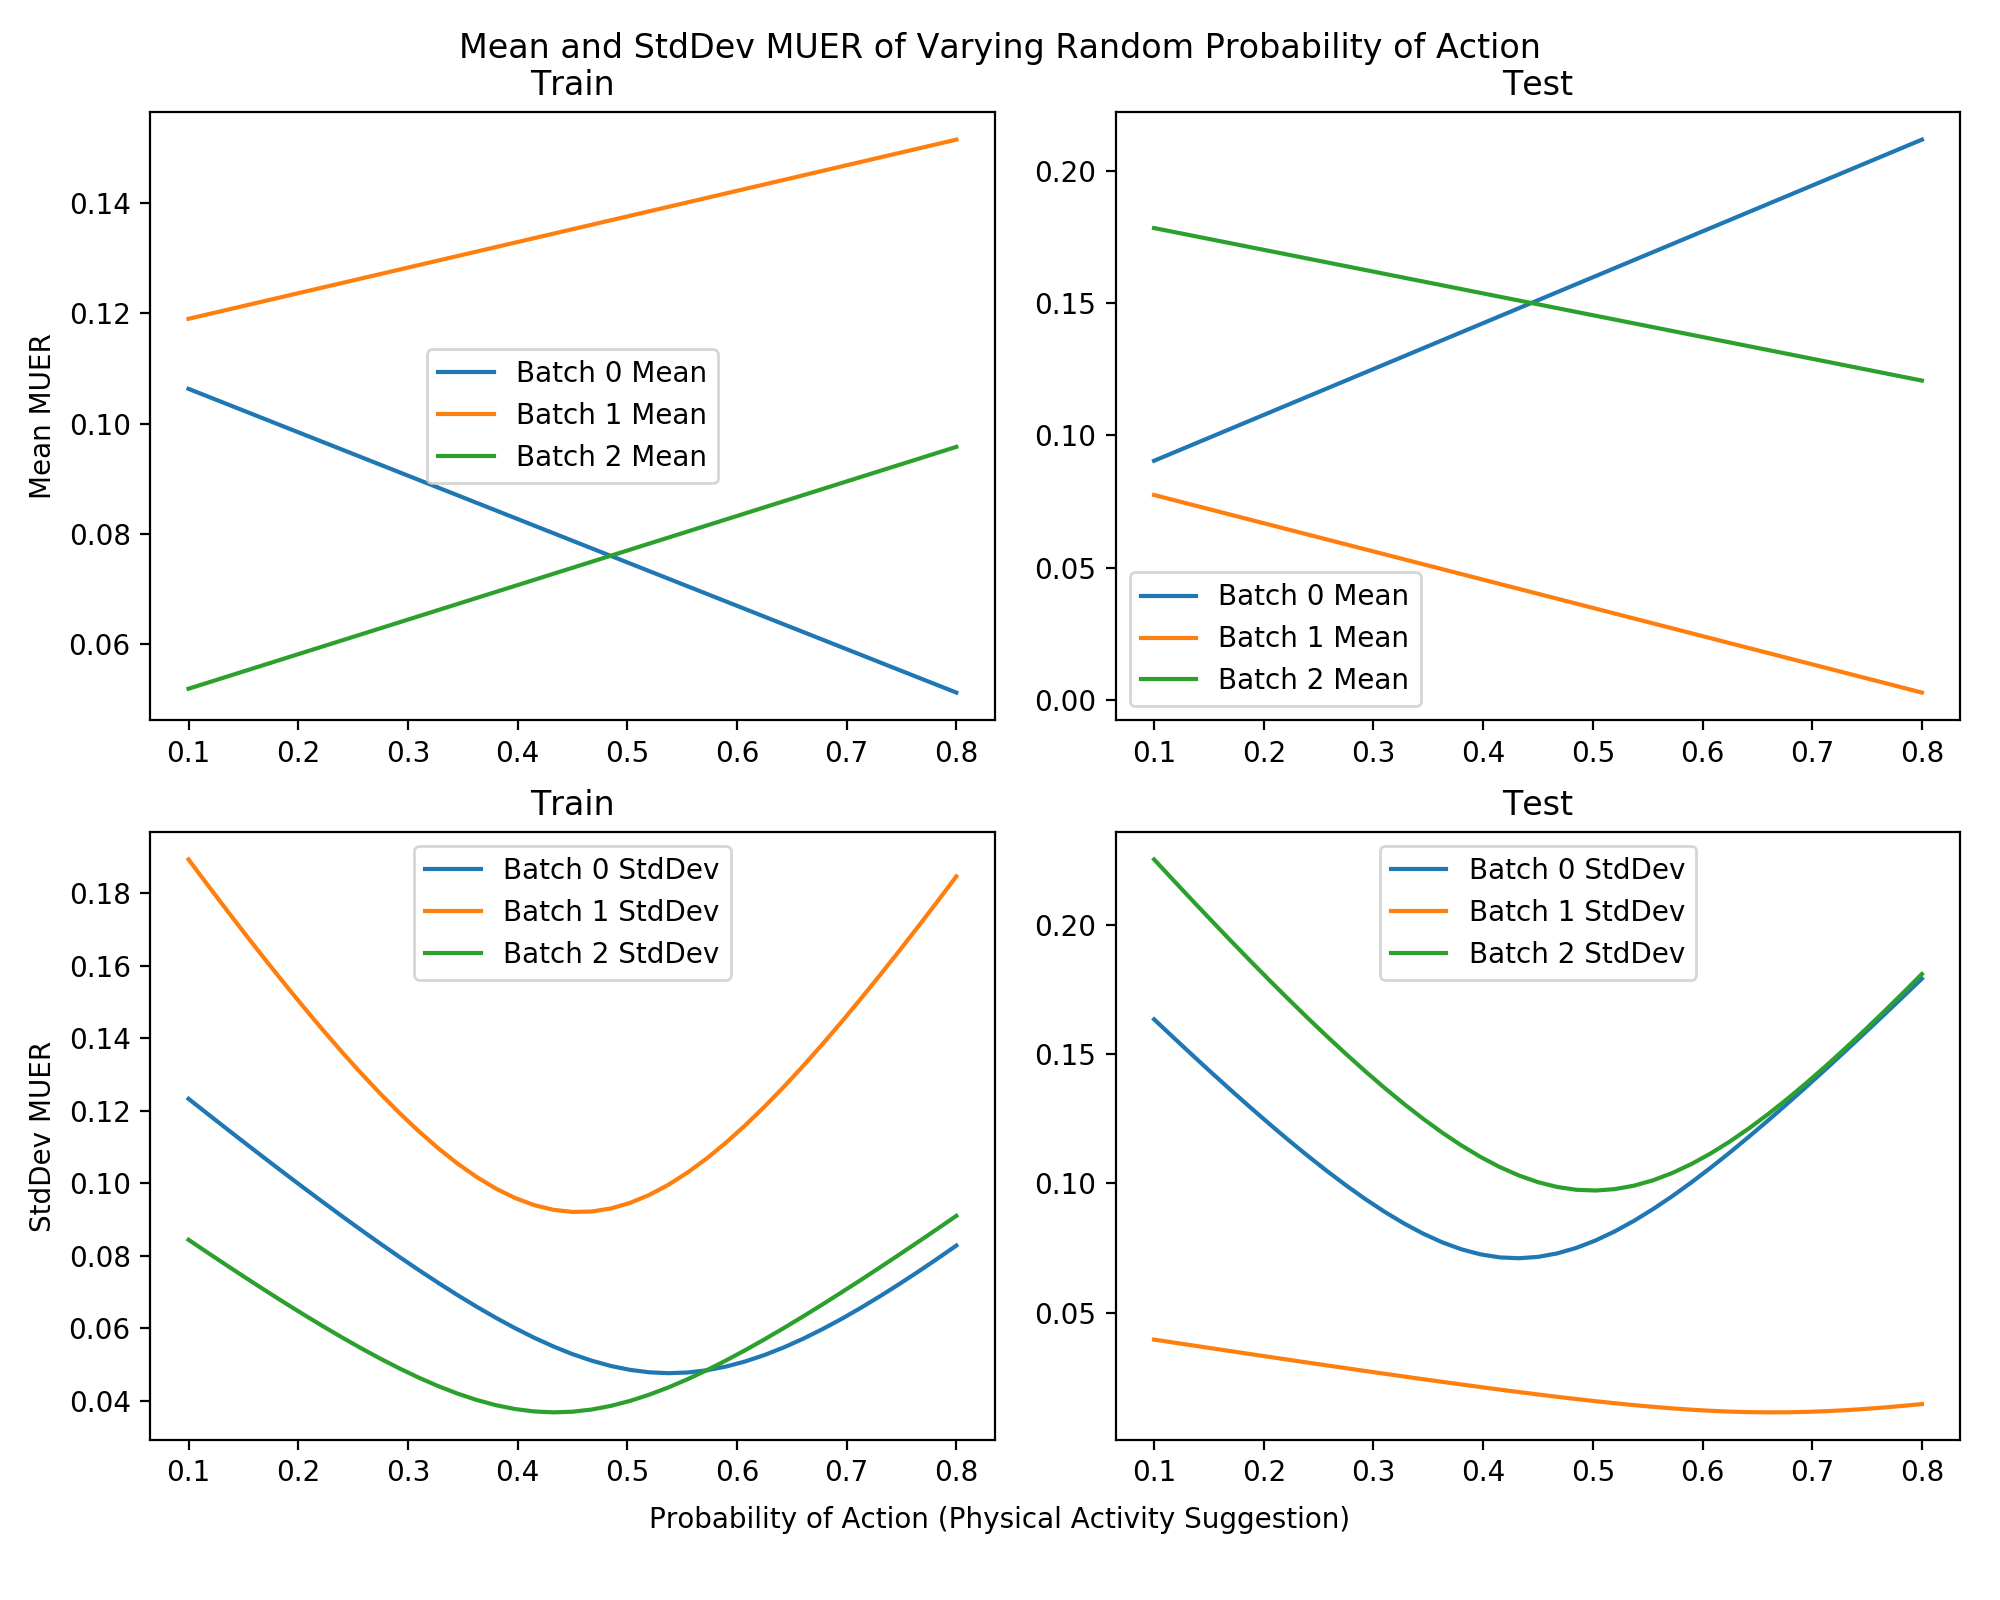
\includegraphics[width=0.8\textwidth,center]{figures/RandomActionVsProbability.png}}
\caption{Overall Regrets for Varying Action Probability $\pi_{(t,d)}$ vs $MUER$}
\label{RandomActionVsProbability}
\end{figure}


\begin{figure}[H]
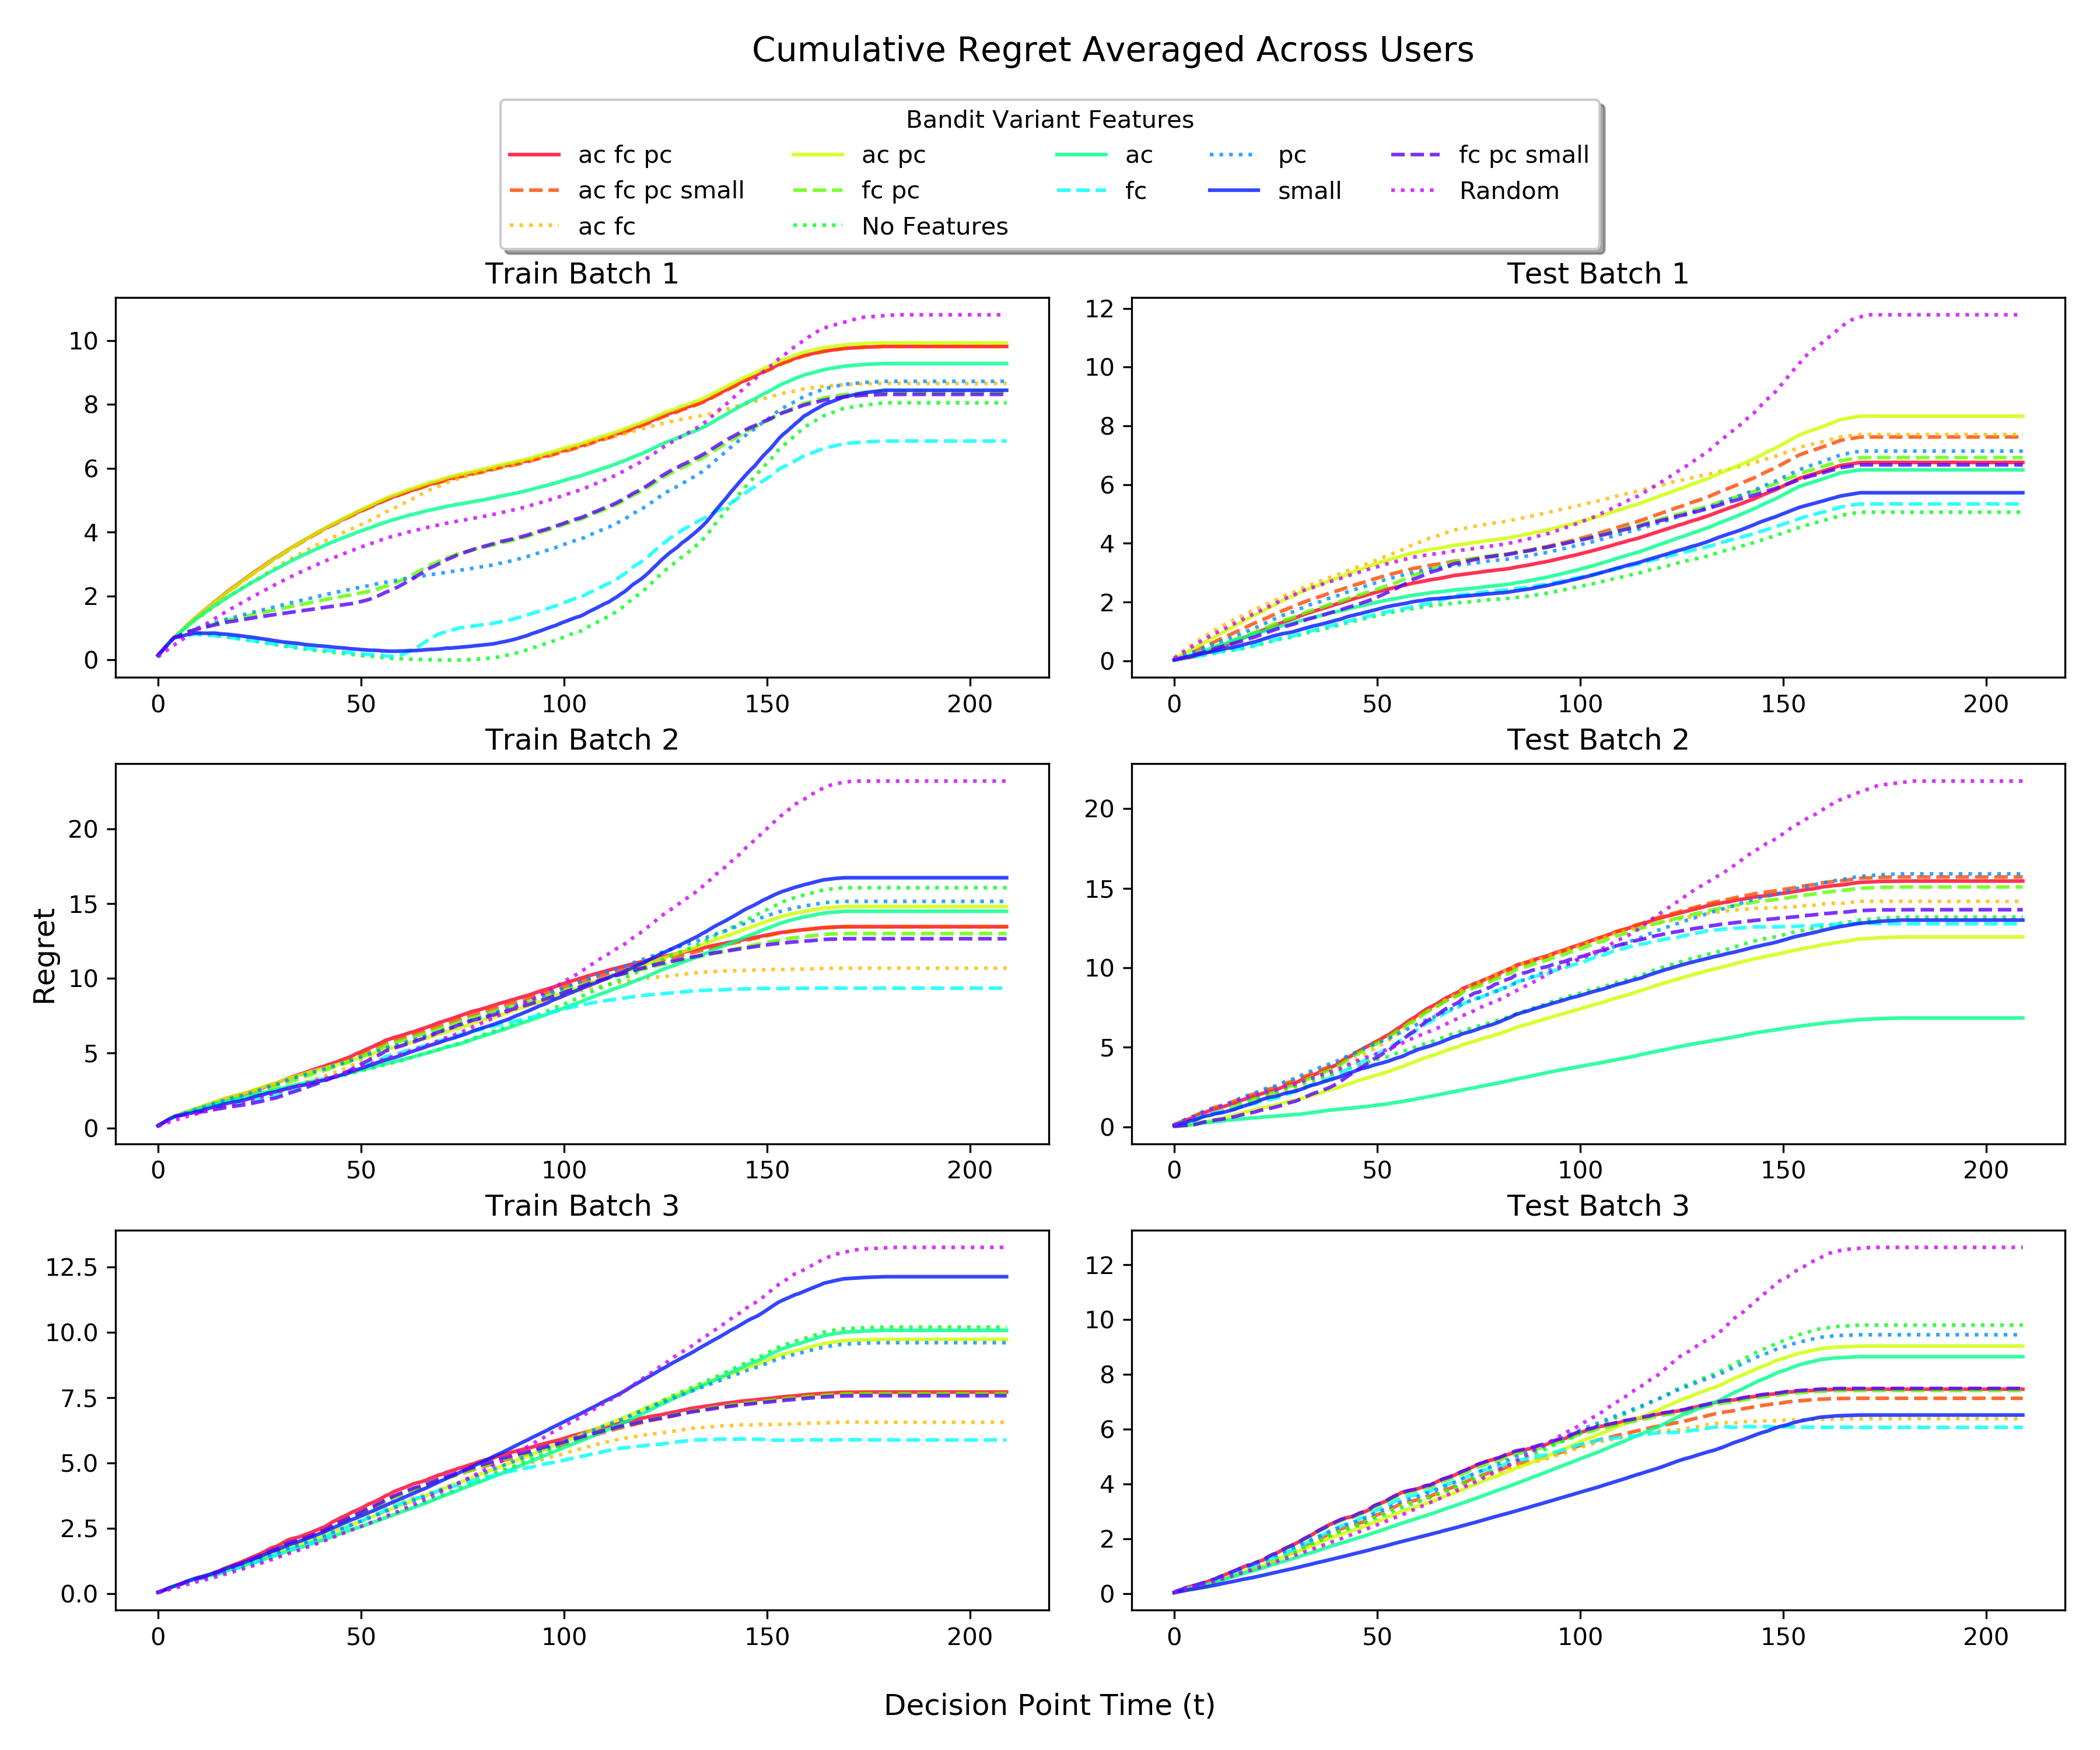
\includegraphics[width=1.35\textwidth,center]{figures/cum_regret_comparison.png}%
\caption{Cumulative Regrets for all Bandit Variants, Separated by Batch}
\label{Cumulative Regrets for all Bandit Variants, Separated by Batch}
\end{figure}


\section{Quality Metric Figures}
\label{Quality Metric Figures}

	\ifdraft
	Turn off Draft mode to display figures!
	\else

	\begin{figure}[H]
	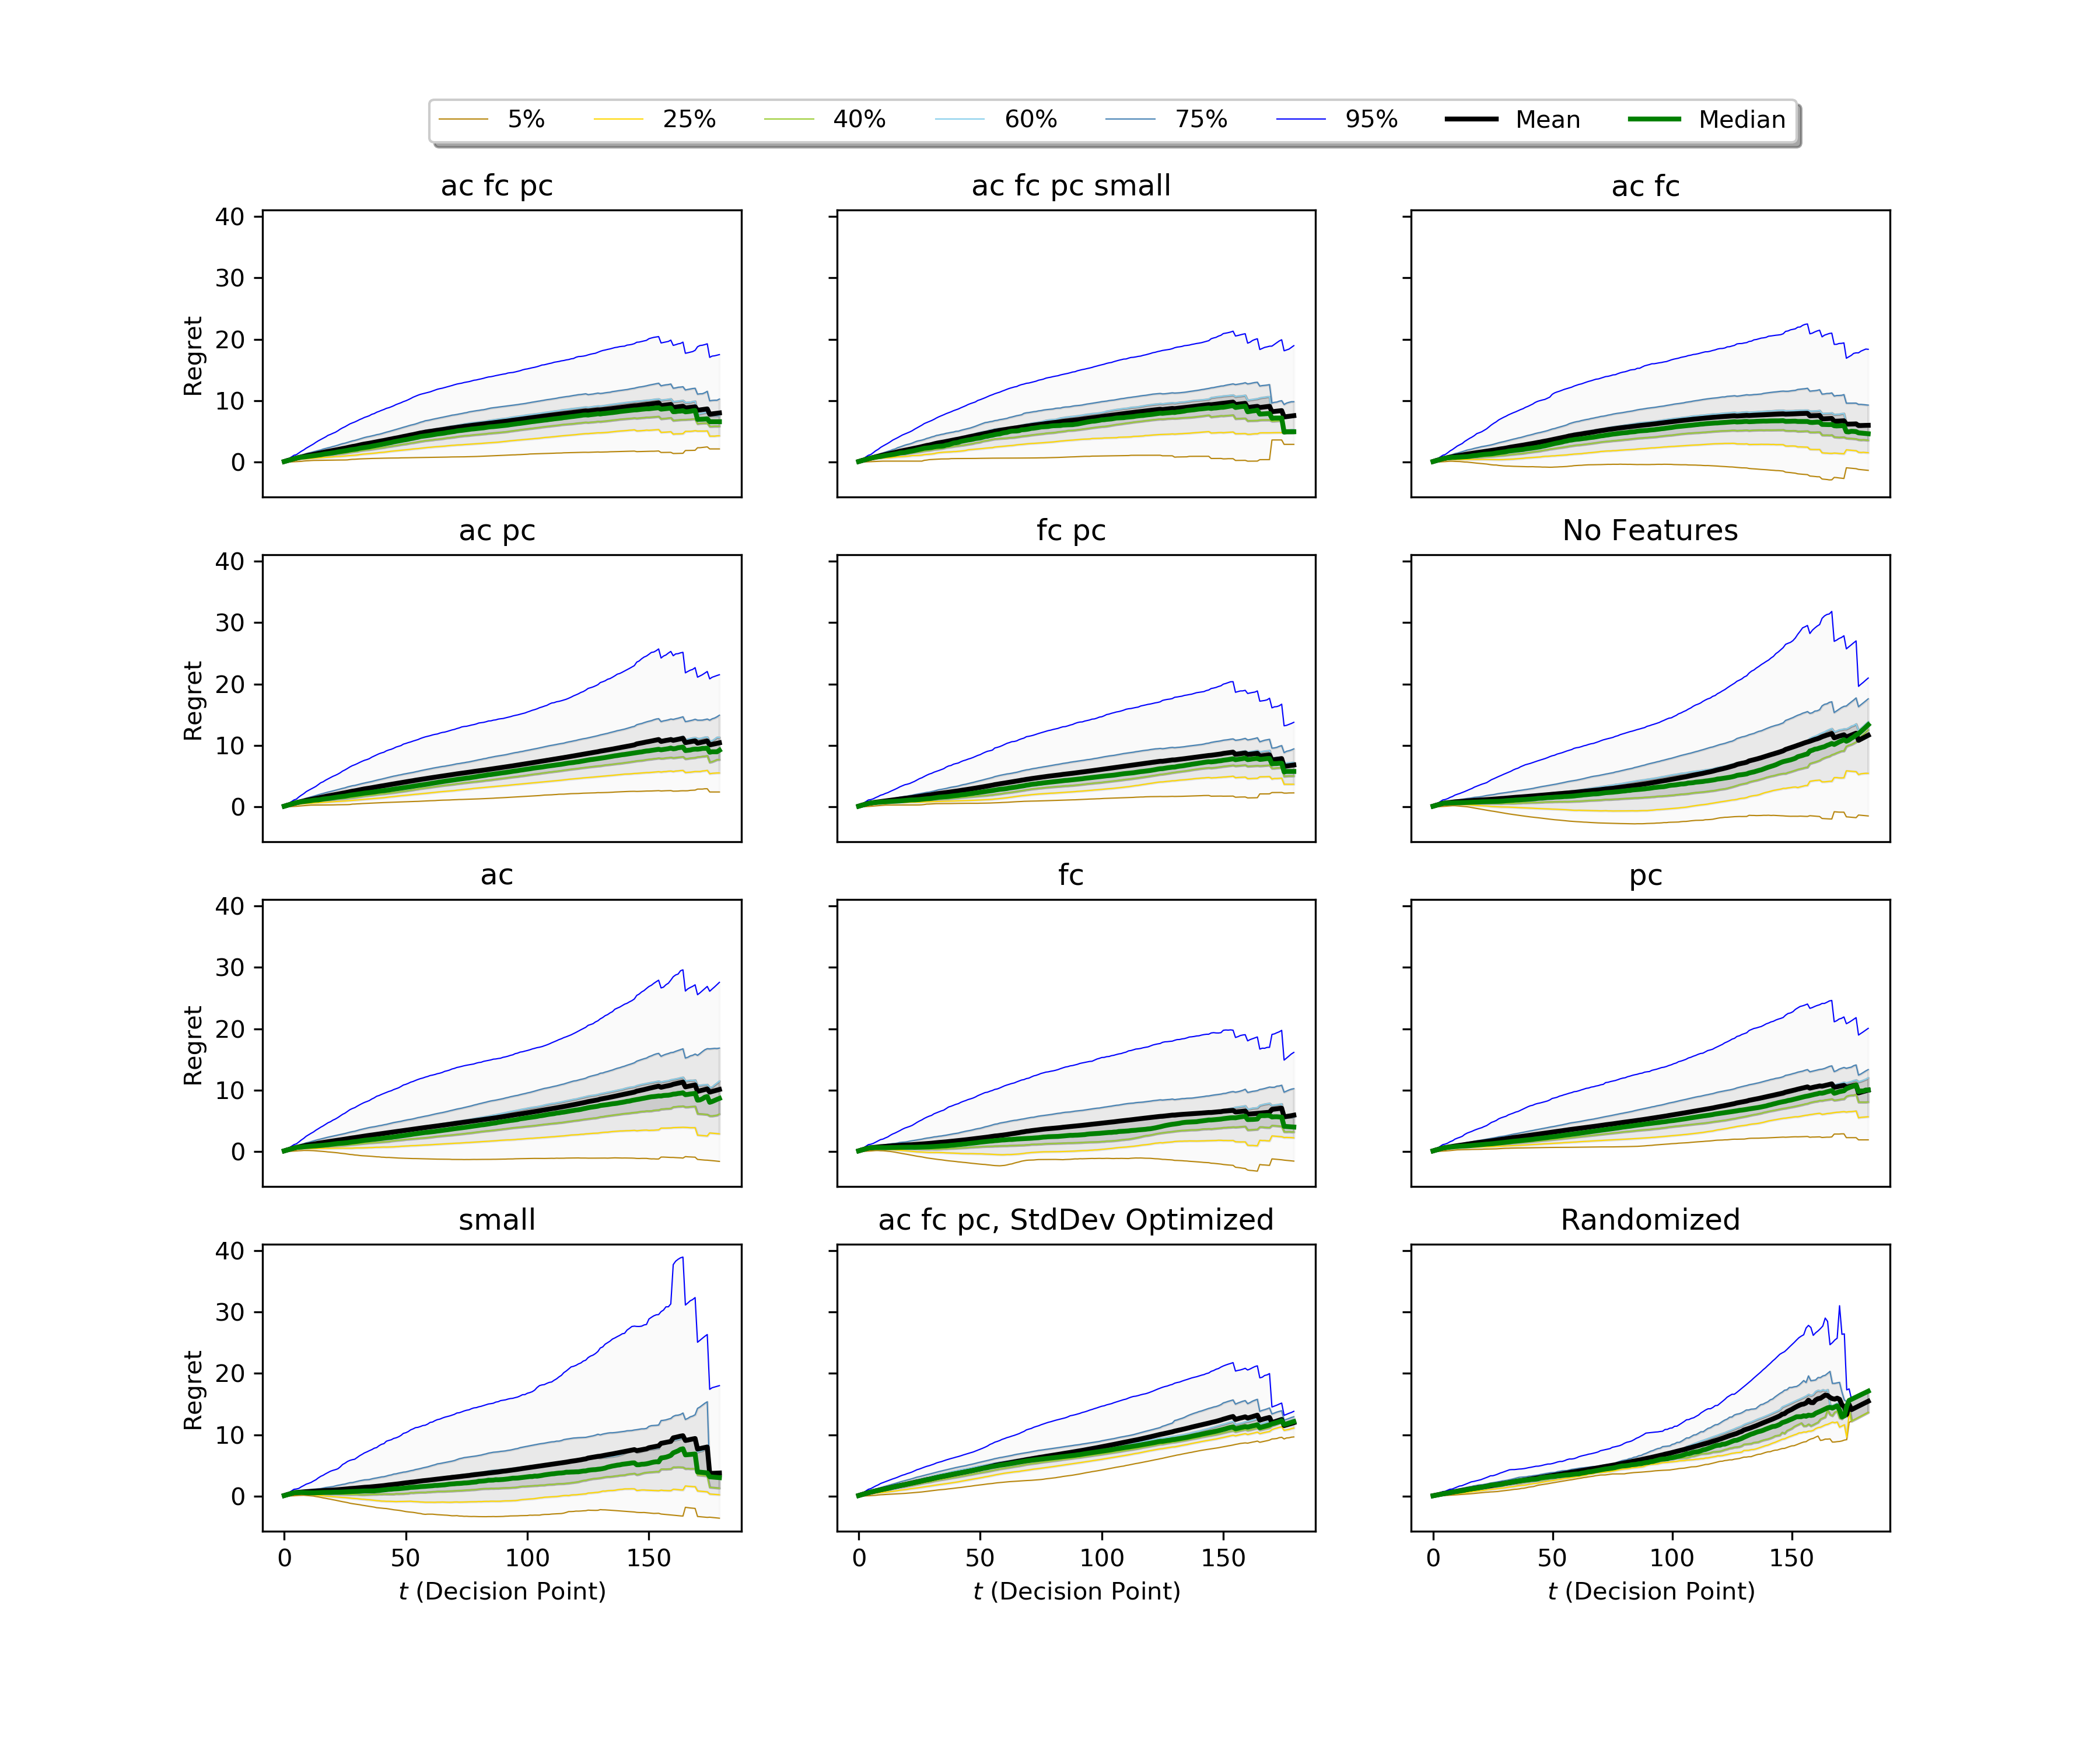
\includegraphics[width=1.5\textwidth,center]{figures/QM2train.png}%
	\caption{Cumulative Regret over Decision Point for All Users in Optimal Training Batches}
	\label{QM2train}
	\end{figure}

	\begin{figure}[H]
	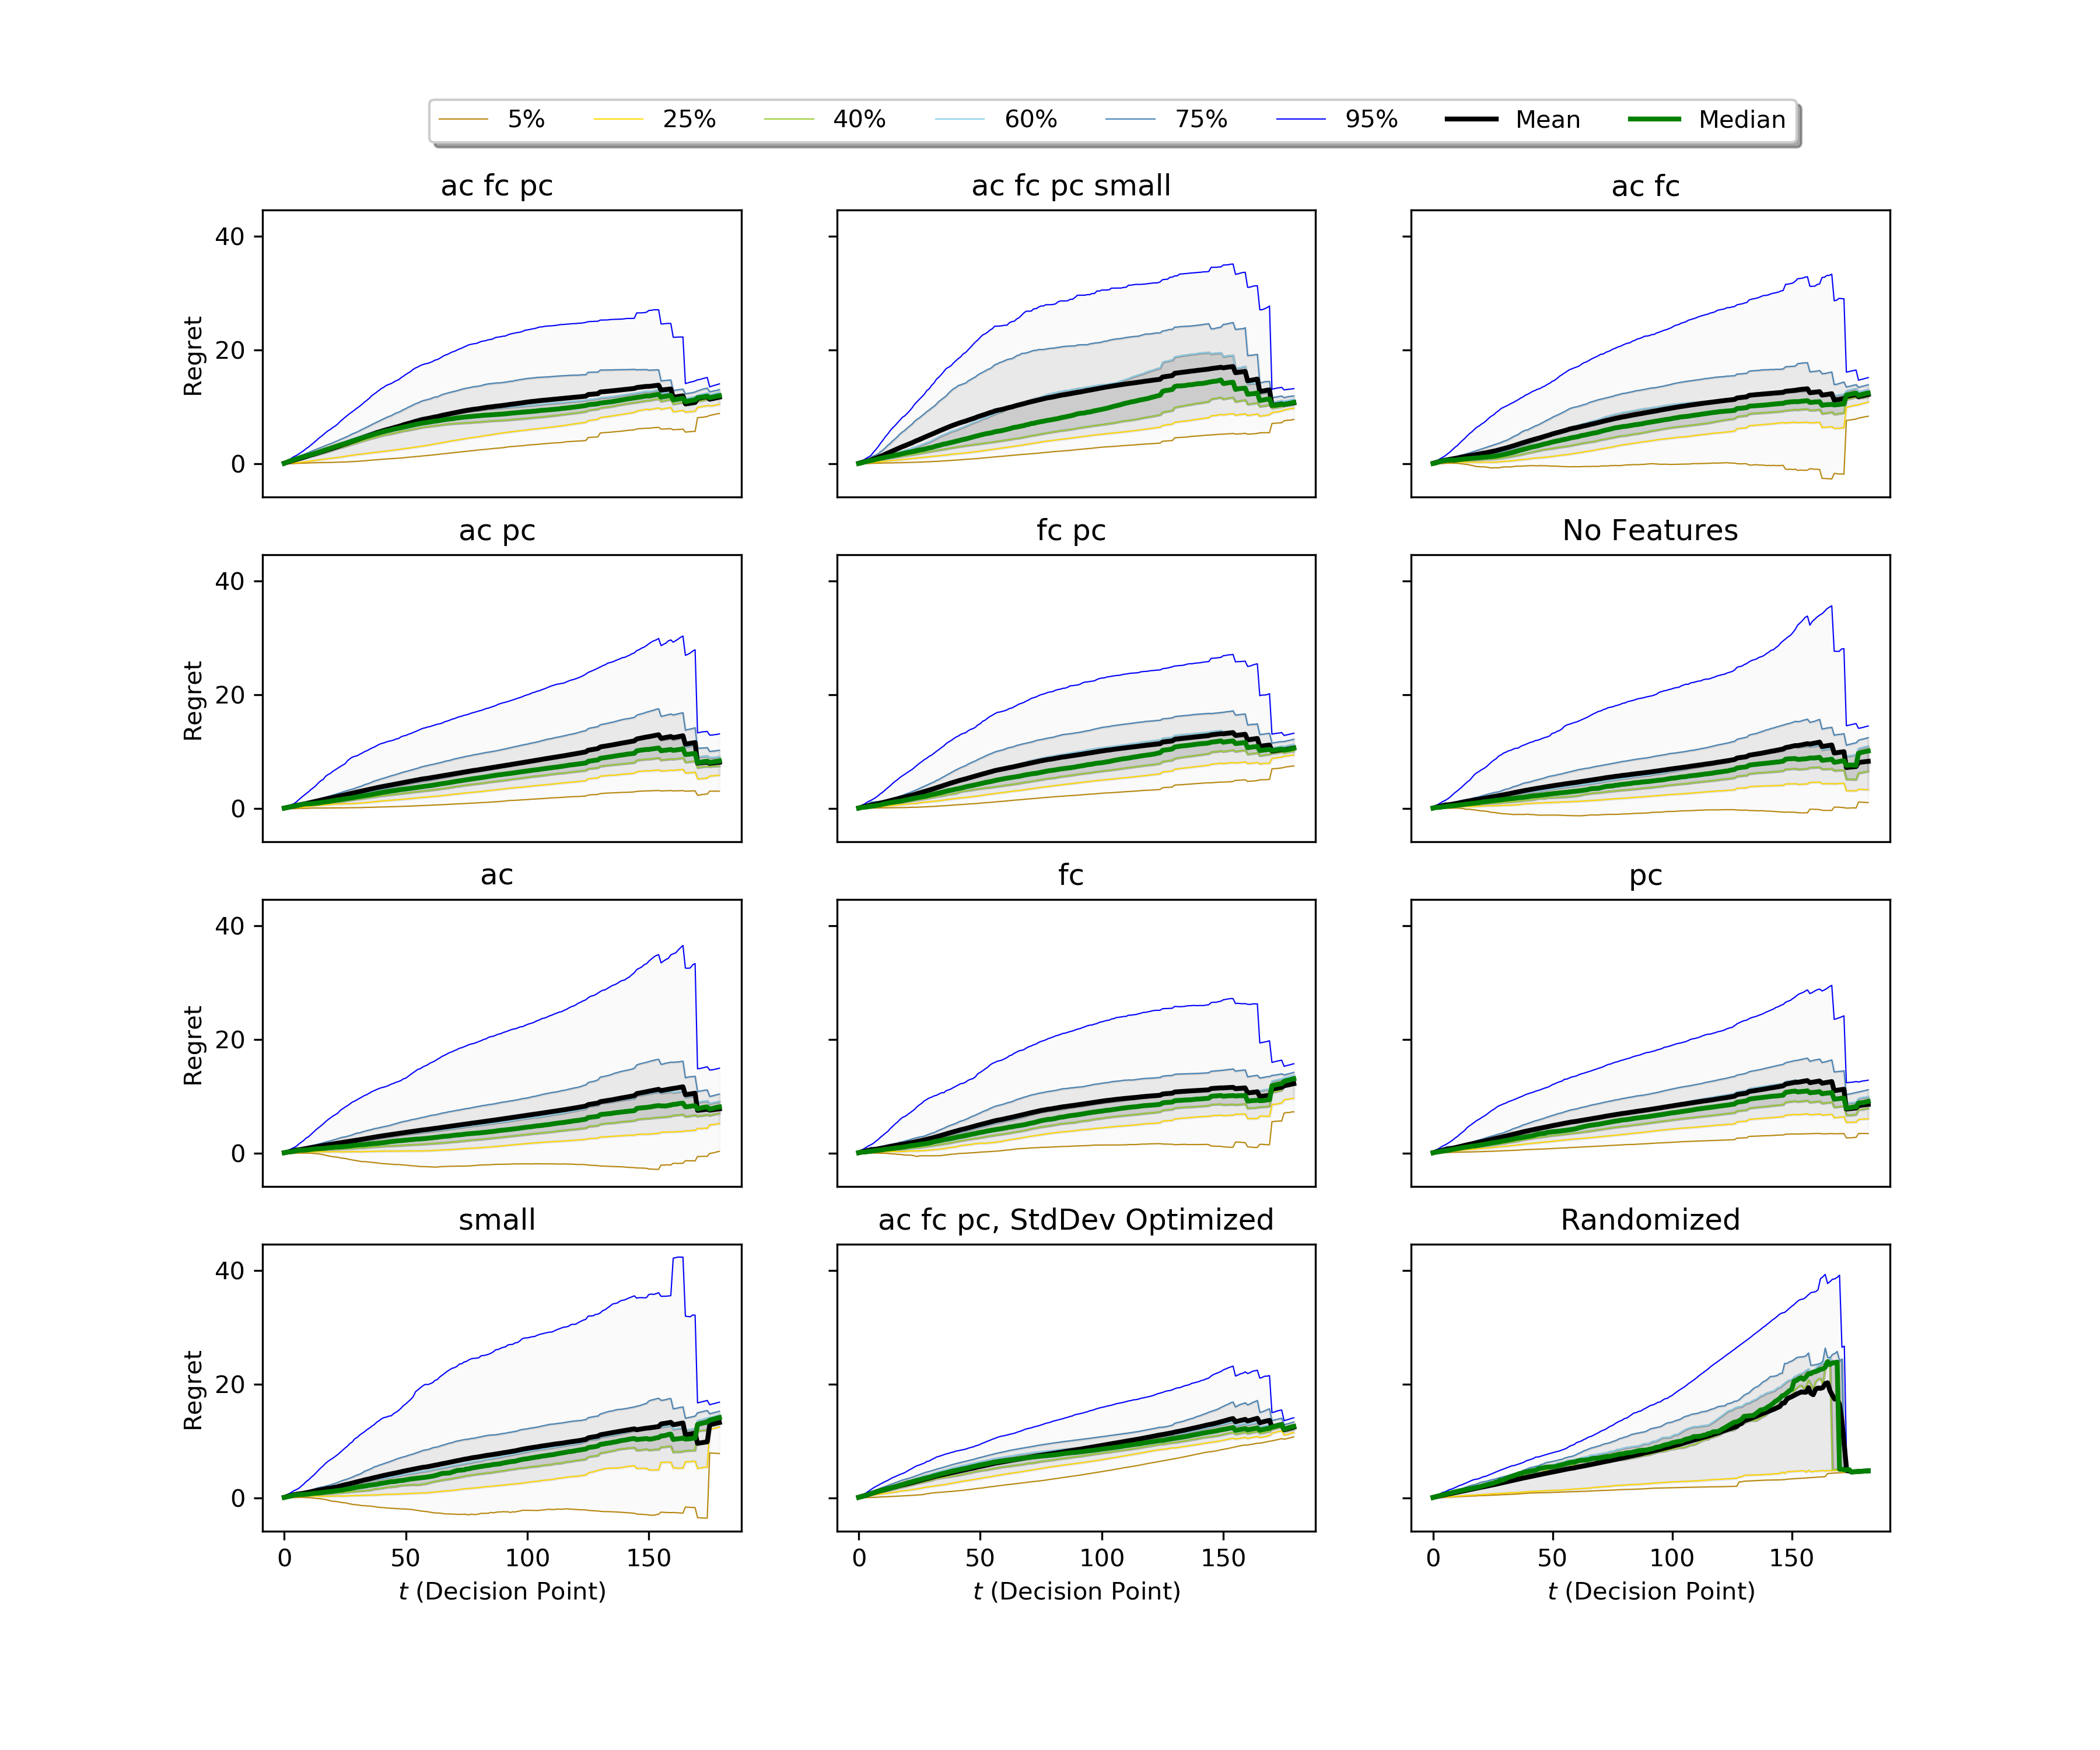
\includegraphics[width=1.5\textwidth,center]{figures/QM2test.png}%
	\caption{Cumulative Regret over Decision Point for All Users in Testing Batches}
	\label{QM2test}
	\end{figure}

	\begin{figure}[H]
	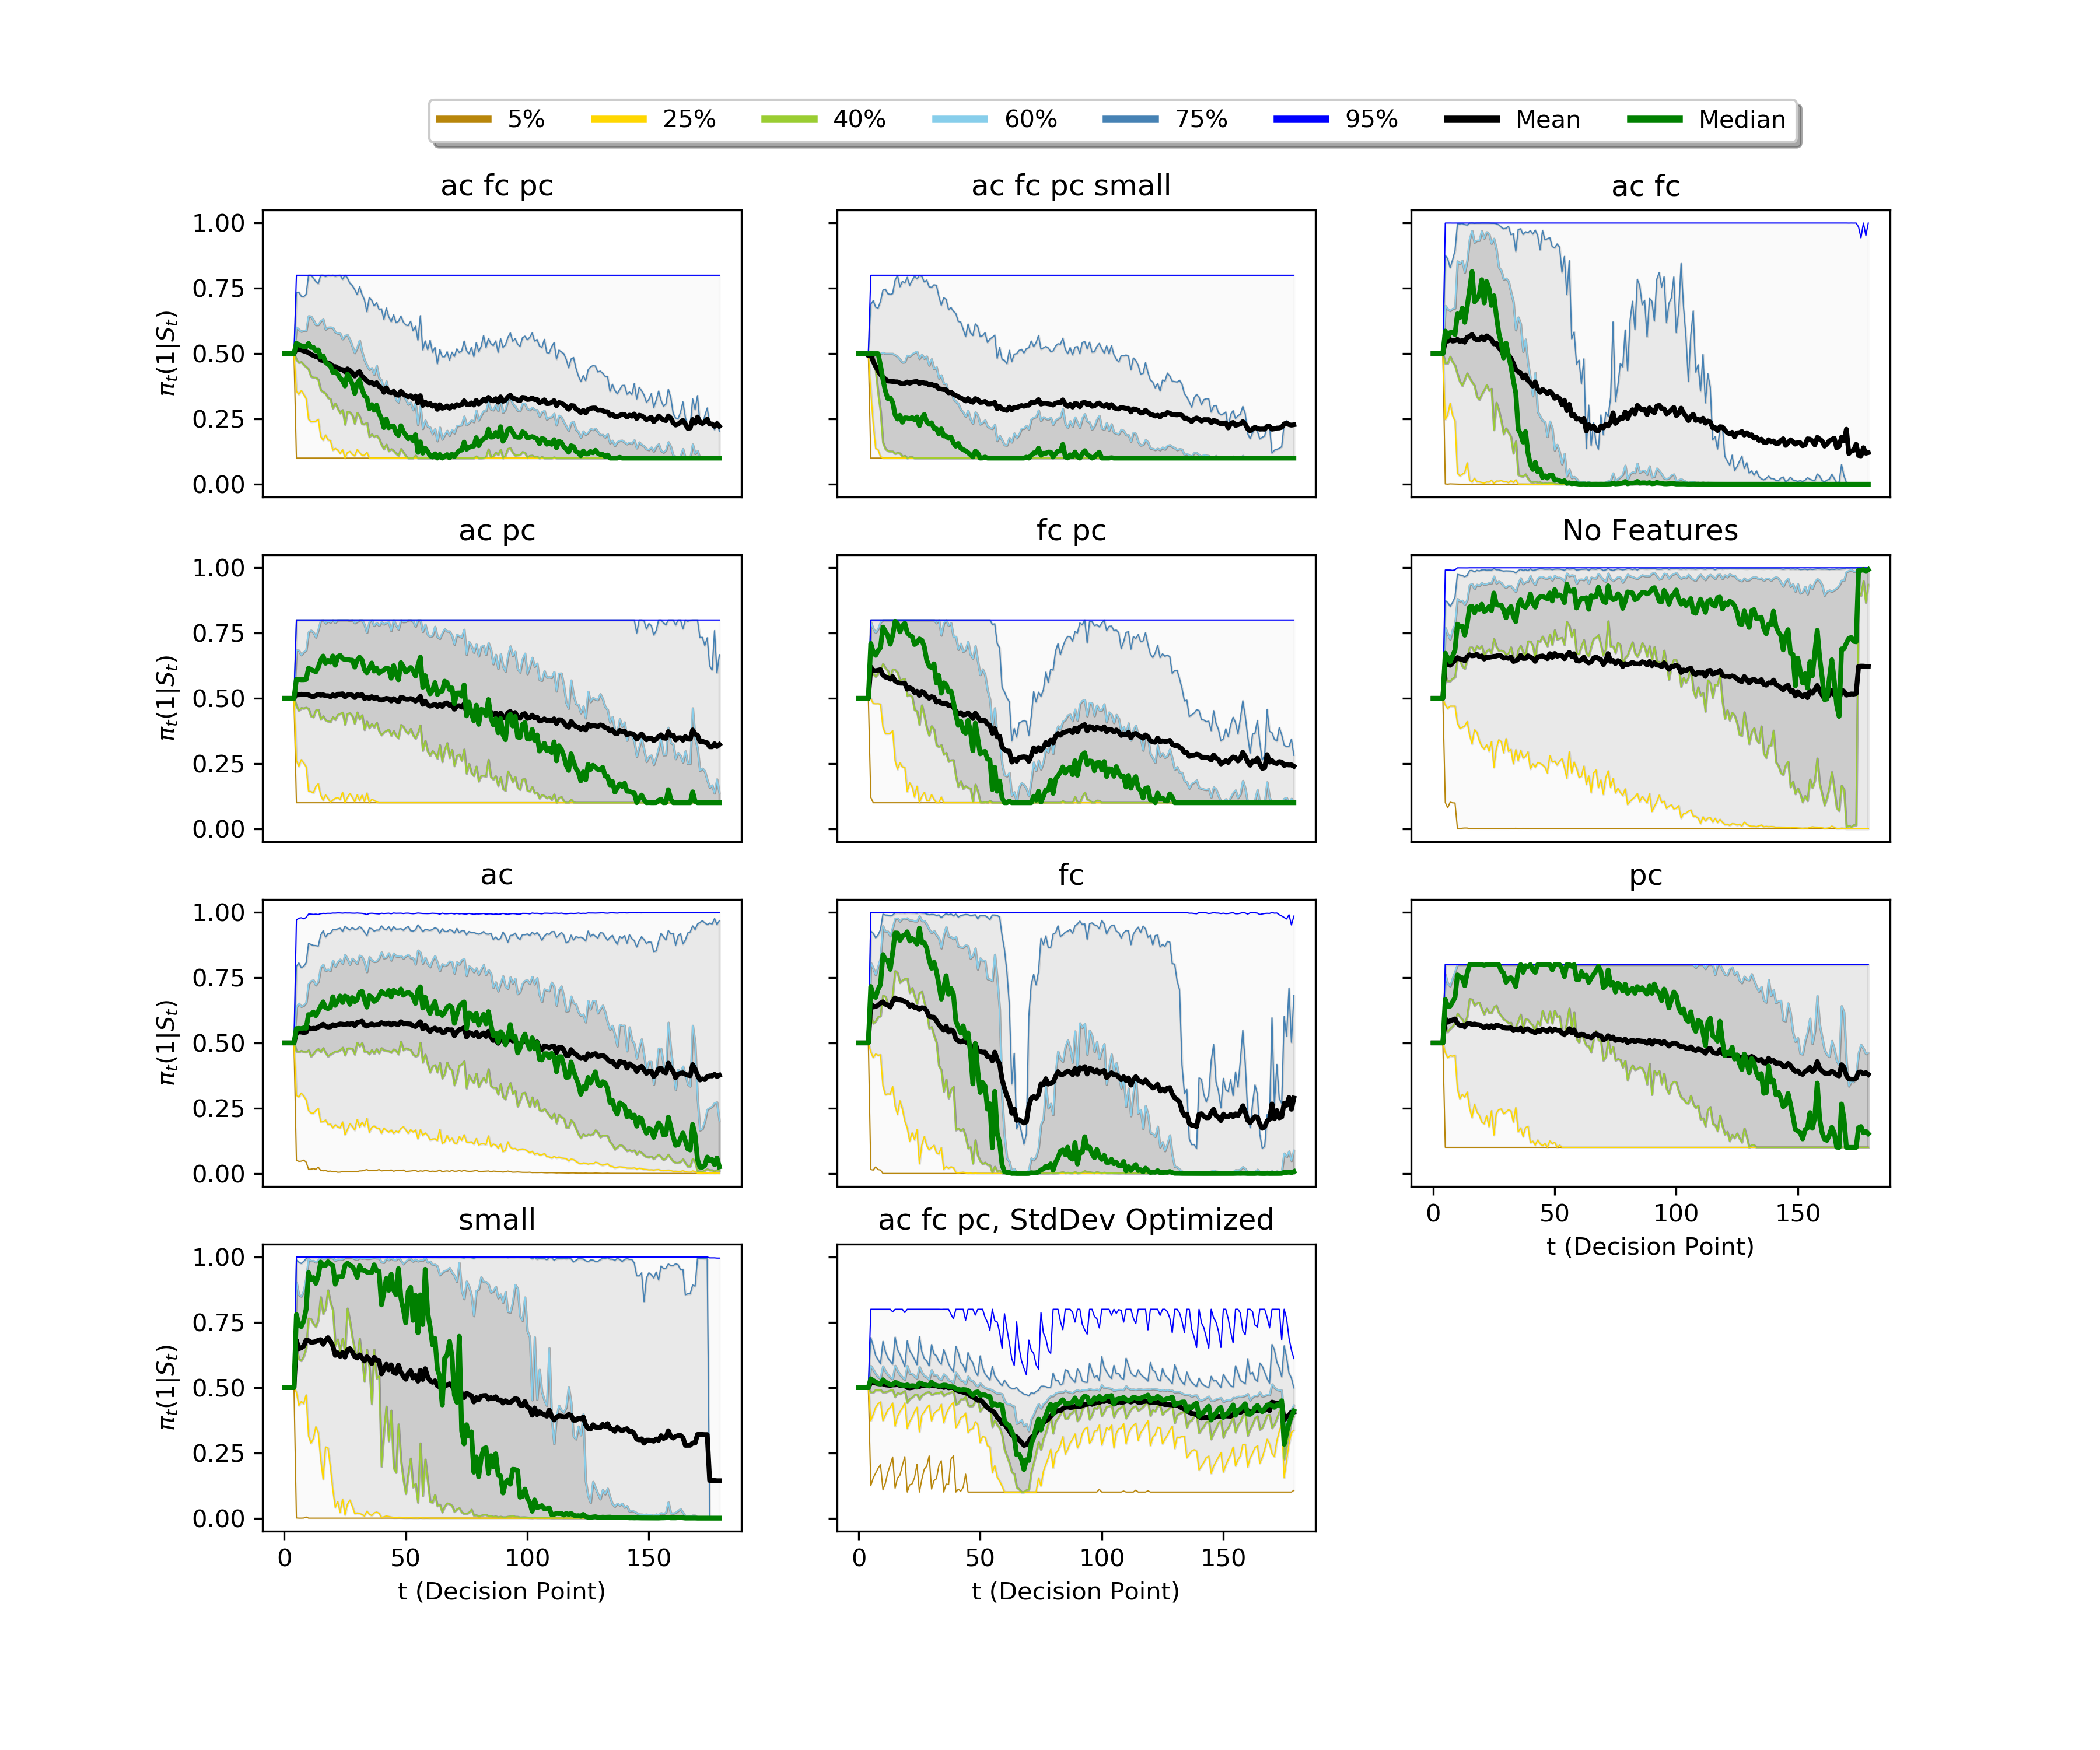
\includegraphics[width=1.5\textwidth,center]{figures/QM3train.png}%
	\caption{Action Probability over Users in Optimal Training Batches}
	\label{QM3train}
	\end{figure}

	\begin{figure}[H]
	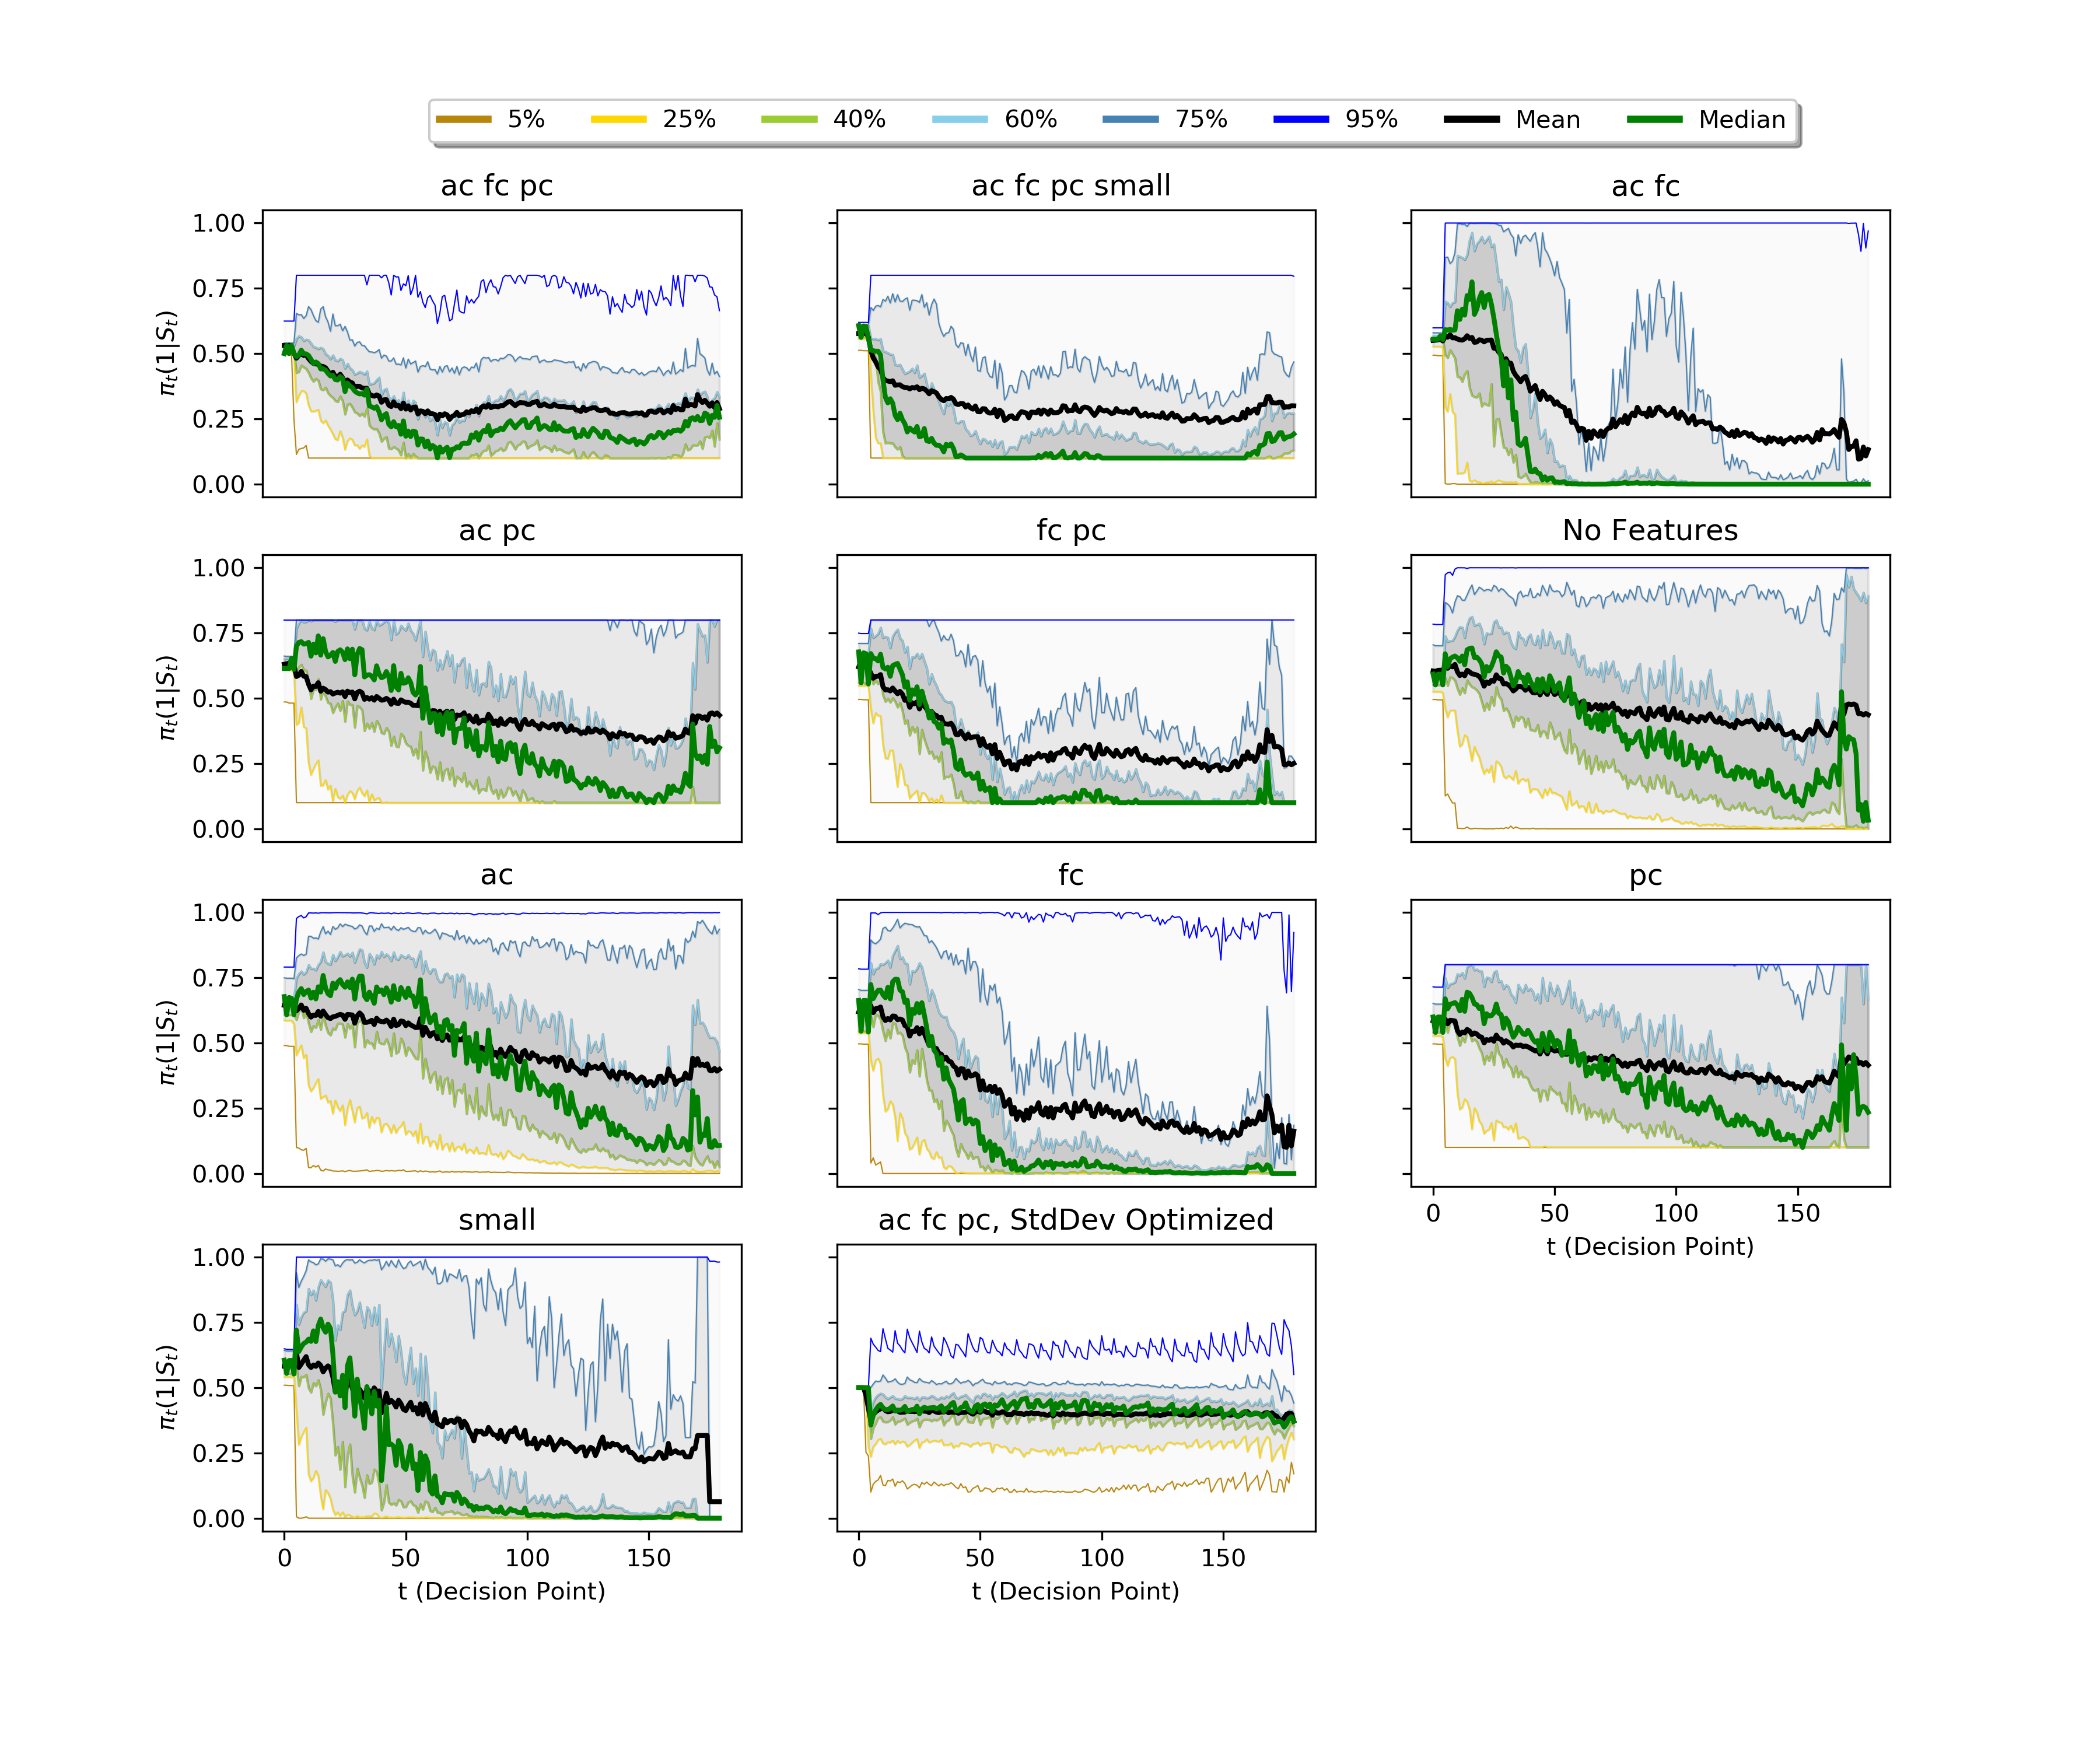
\includegraphics[width=1.5\textwidth,center]{figures/QM3test.png}%
	\caption{Action Probability over Users in Testing Batches}
	\label{QM3test}
	\end{figure}

	\begin{figure}[H]
	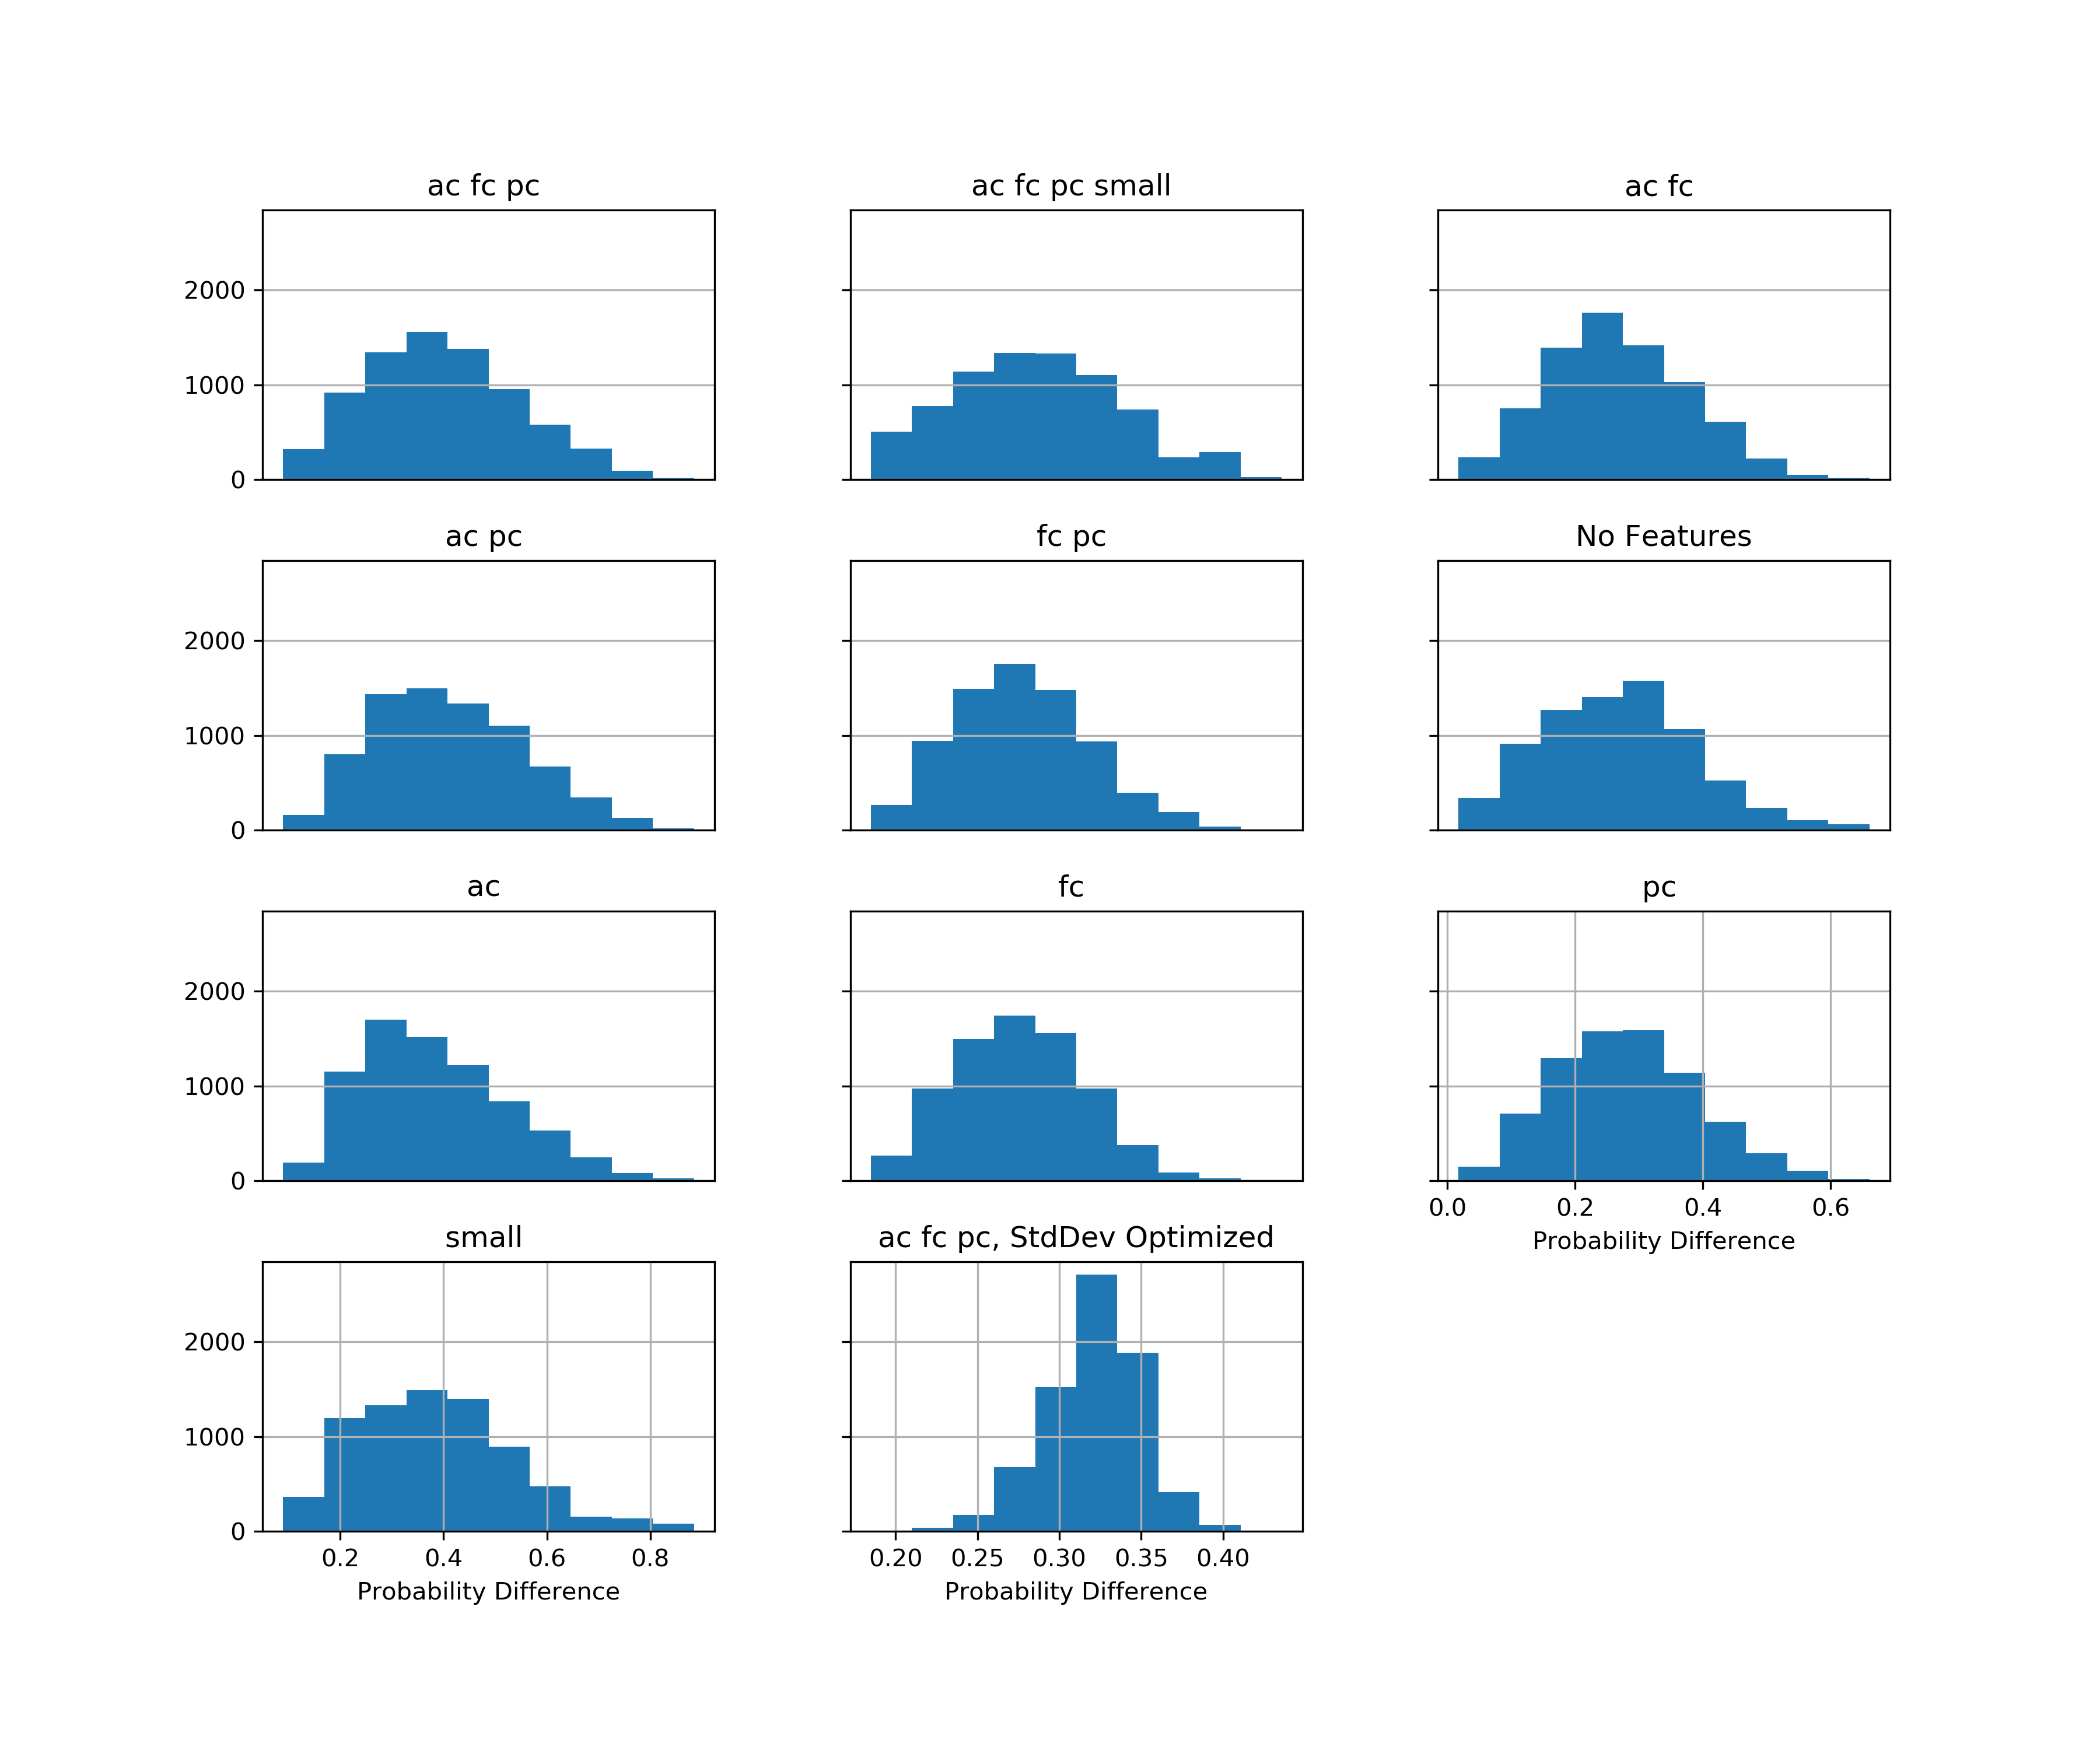
\includegraphics[width=1.5\textwidth,center]{figures/QM5train.png}%
	\caption{|Action Probability - Optimal Probability| Averaged over all $t$ for $7500$ Users in Optimal Training Batches}
	\label{QM5train}
	\end{figure}

	\begin{figure}[H]
	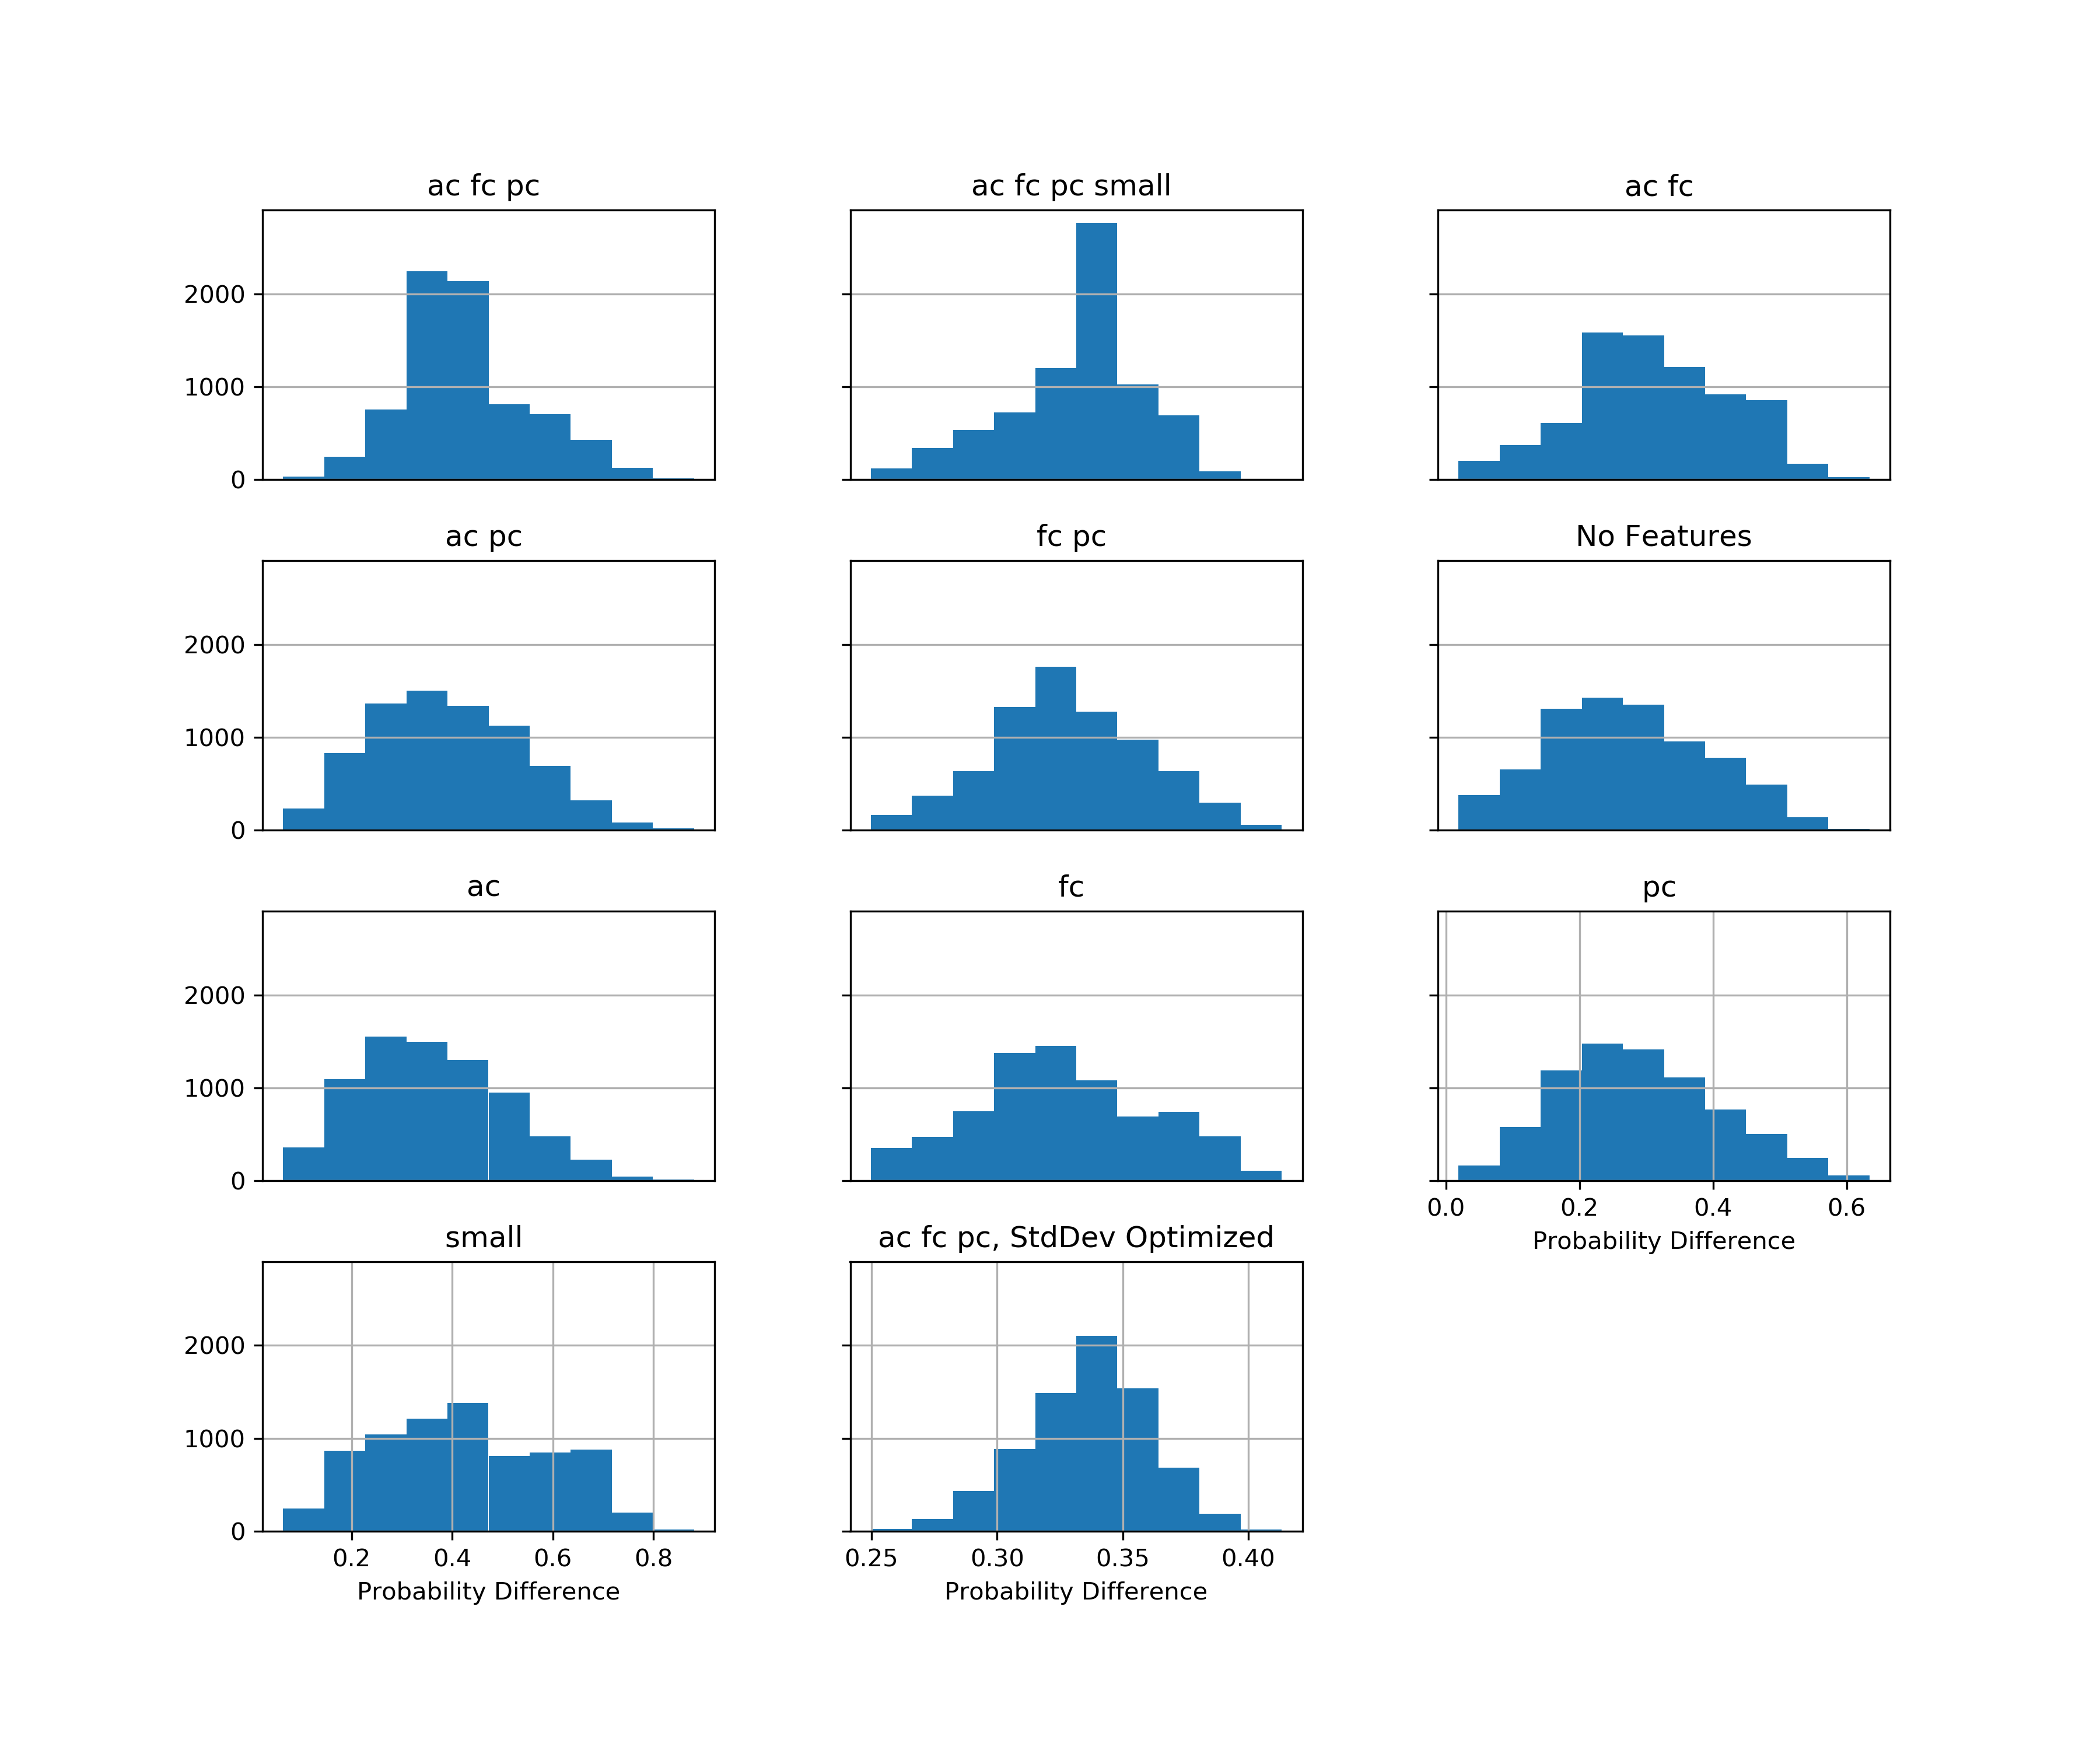
\includegraphics[width=1.5\textwidth,center]{figures/QM5test.png}%
	\caption{|Action Probability - Optimal Probability| Averaged over all $t$ for $7500$ Users in Testing Batches}
	\label{QM5test}
	\end{figure}

	\begin{figure}[H]
	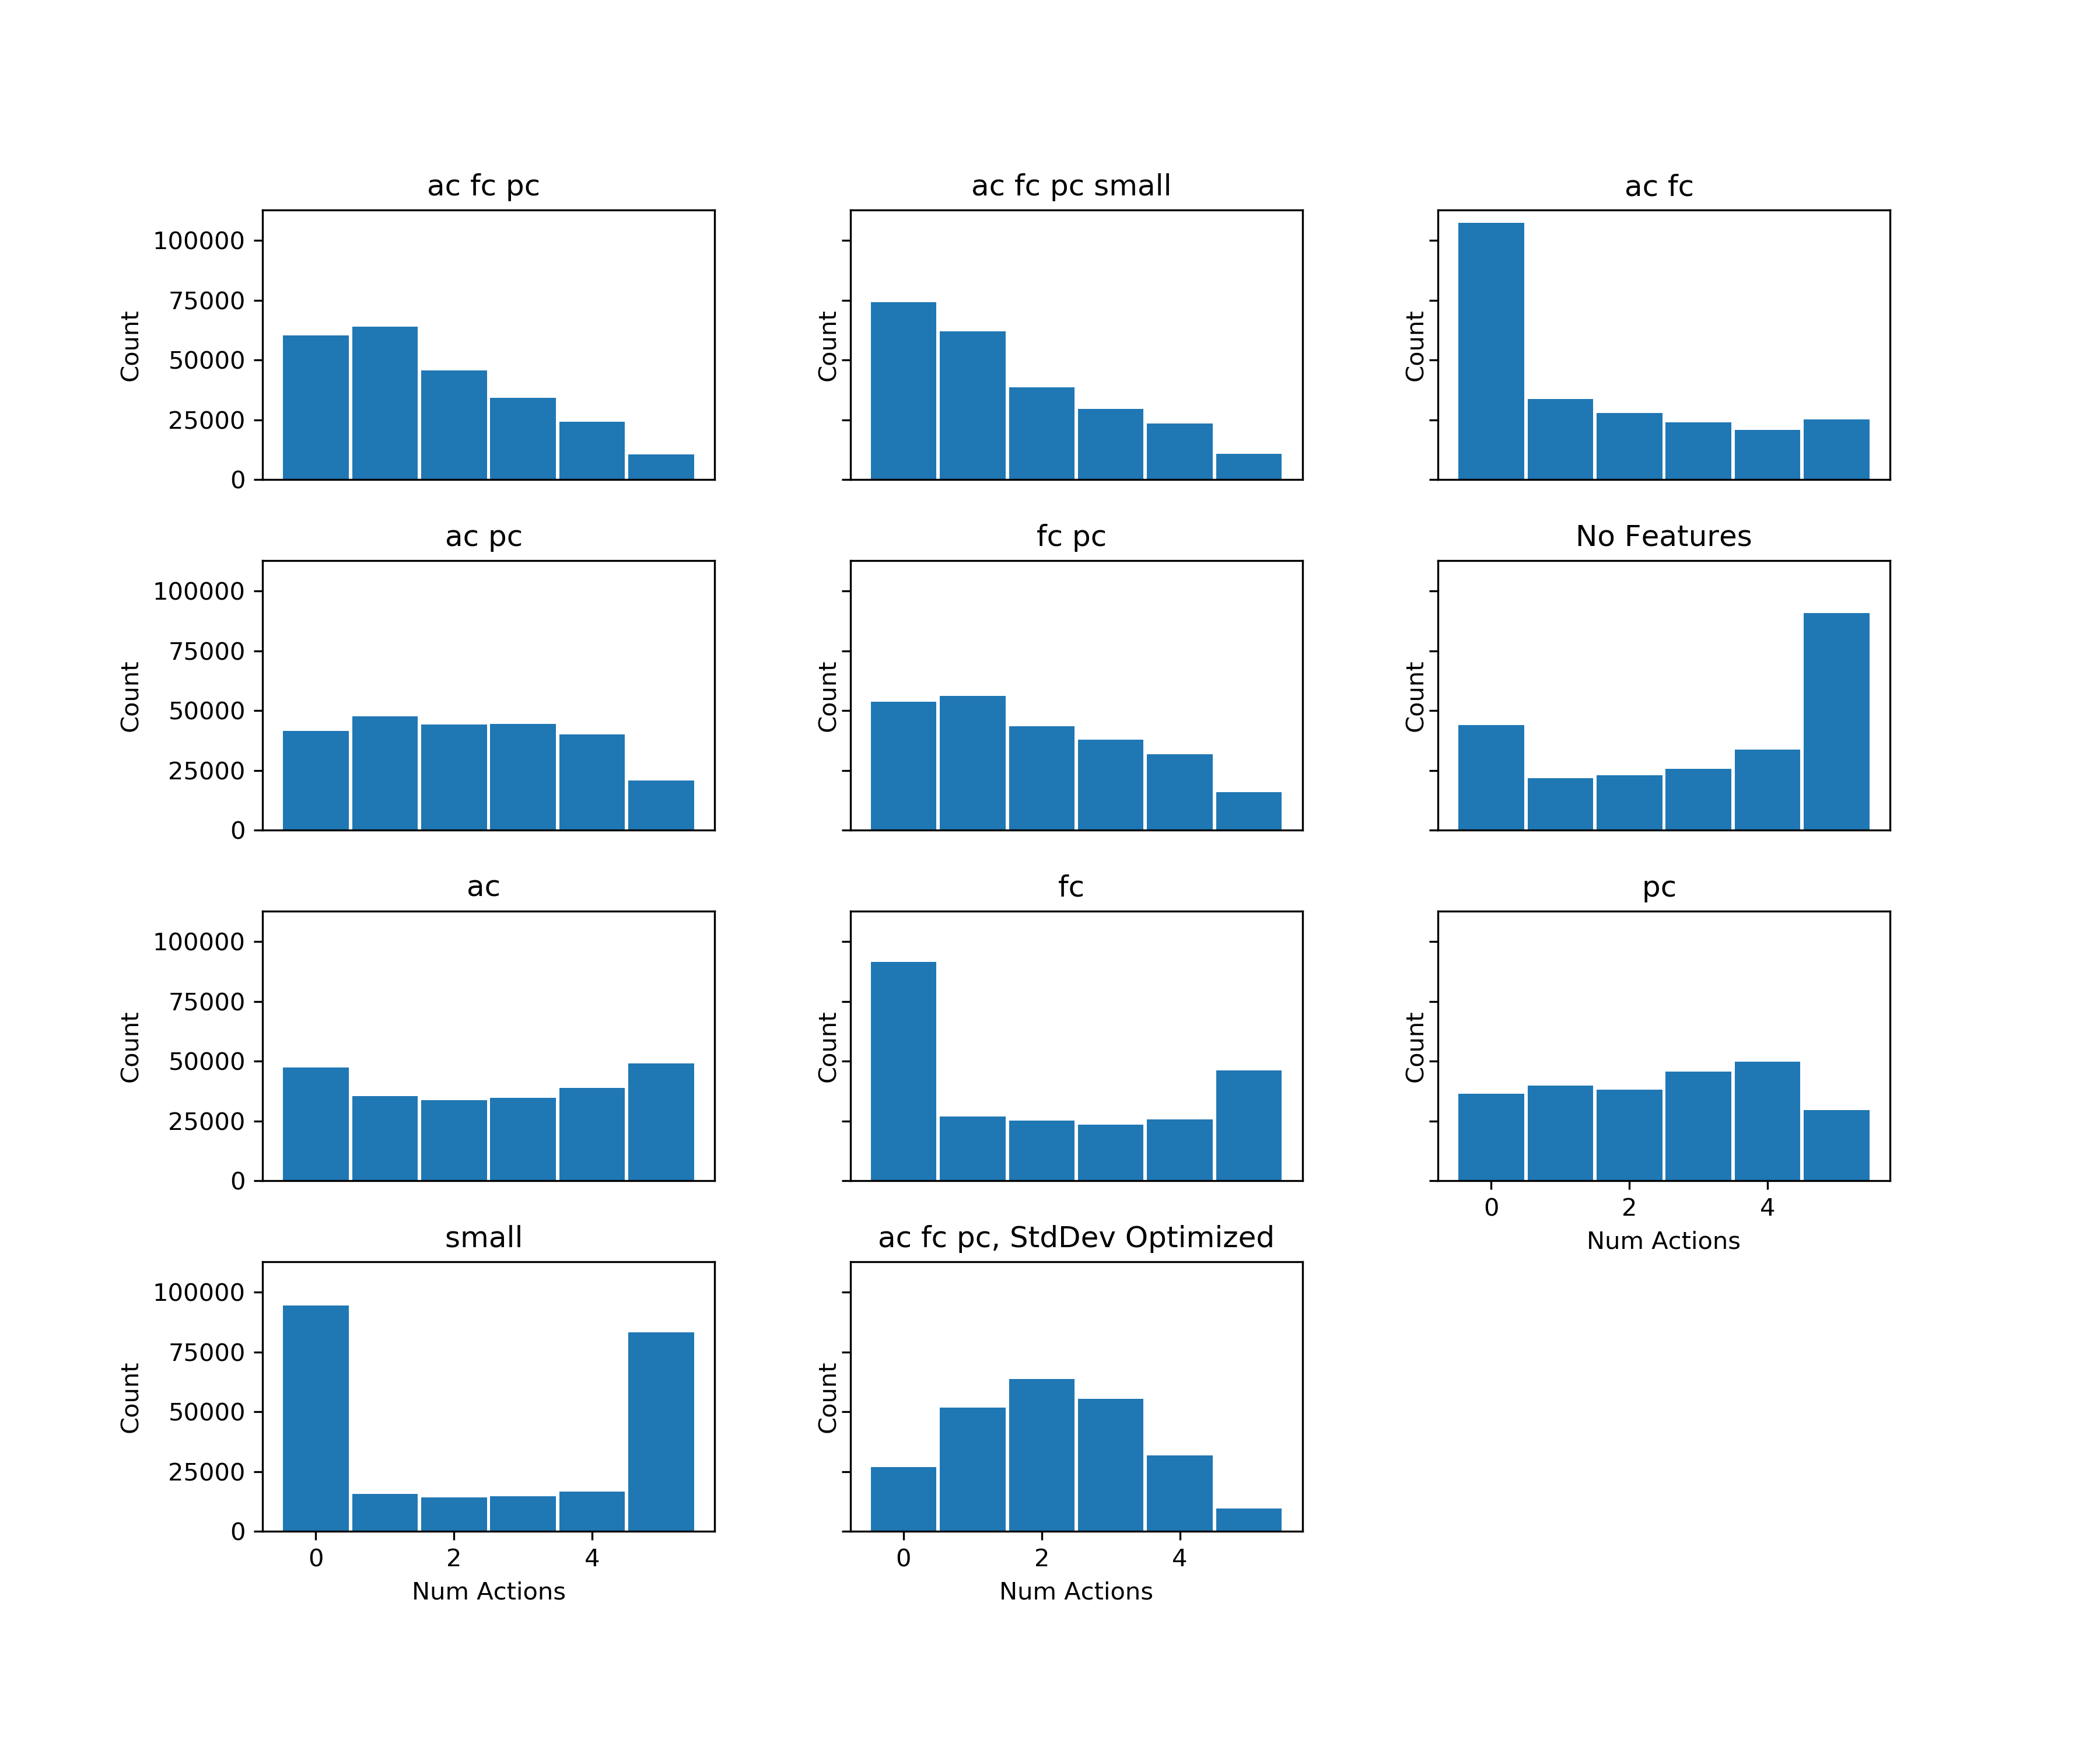
\includegraphics[width=1.5\textwidth,center]{figures/QM6train.png}%
	\caption{Number of Actions per Day across all Users in Optimal Training Batches}
	\label{QM6train}
	\end{figure}

	\begin{figure}[H]
	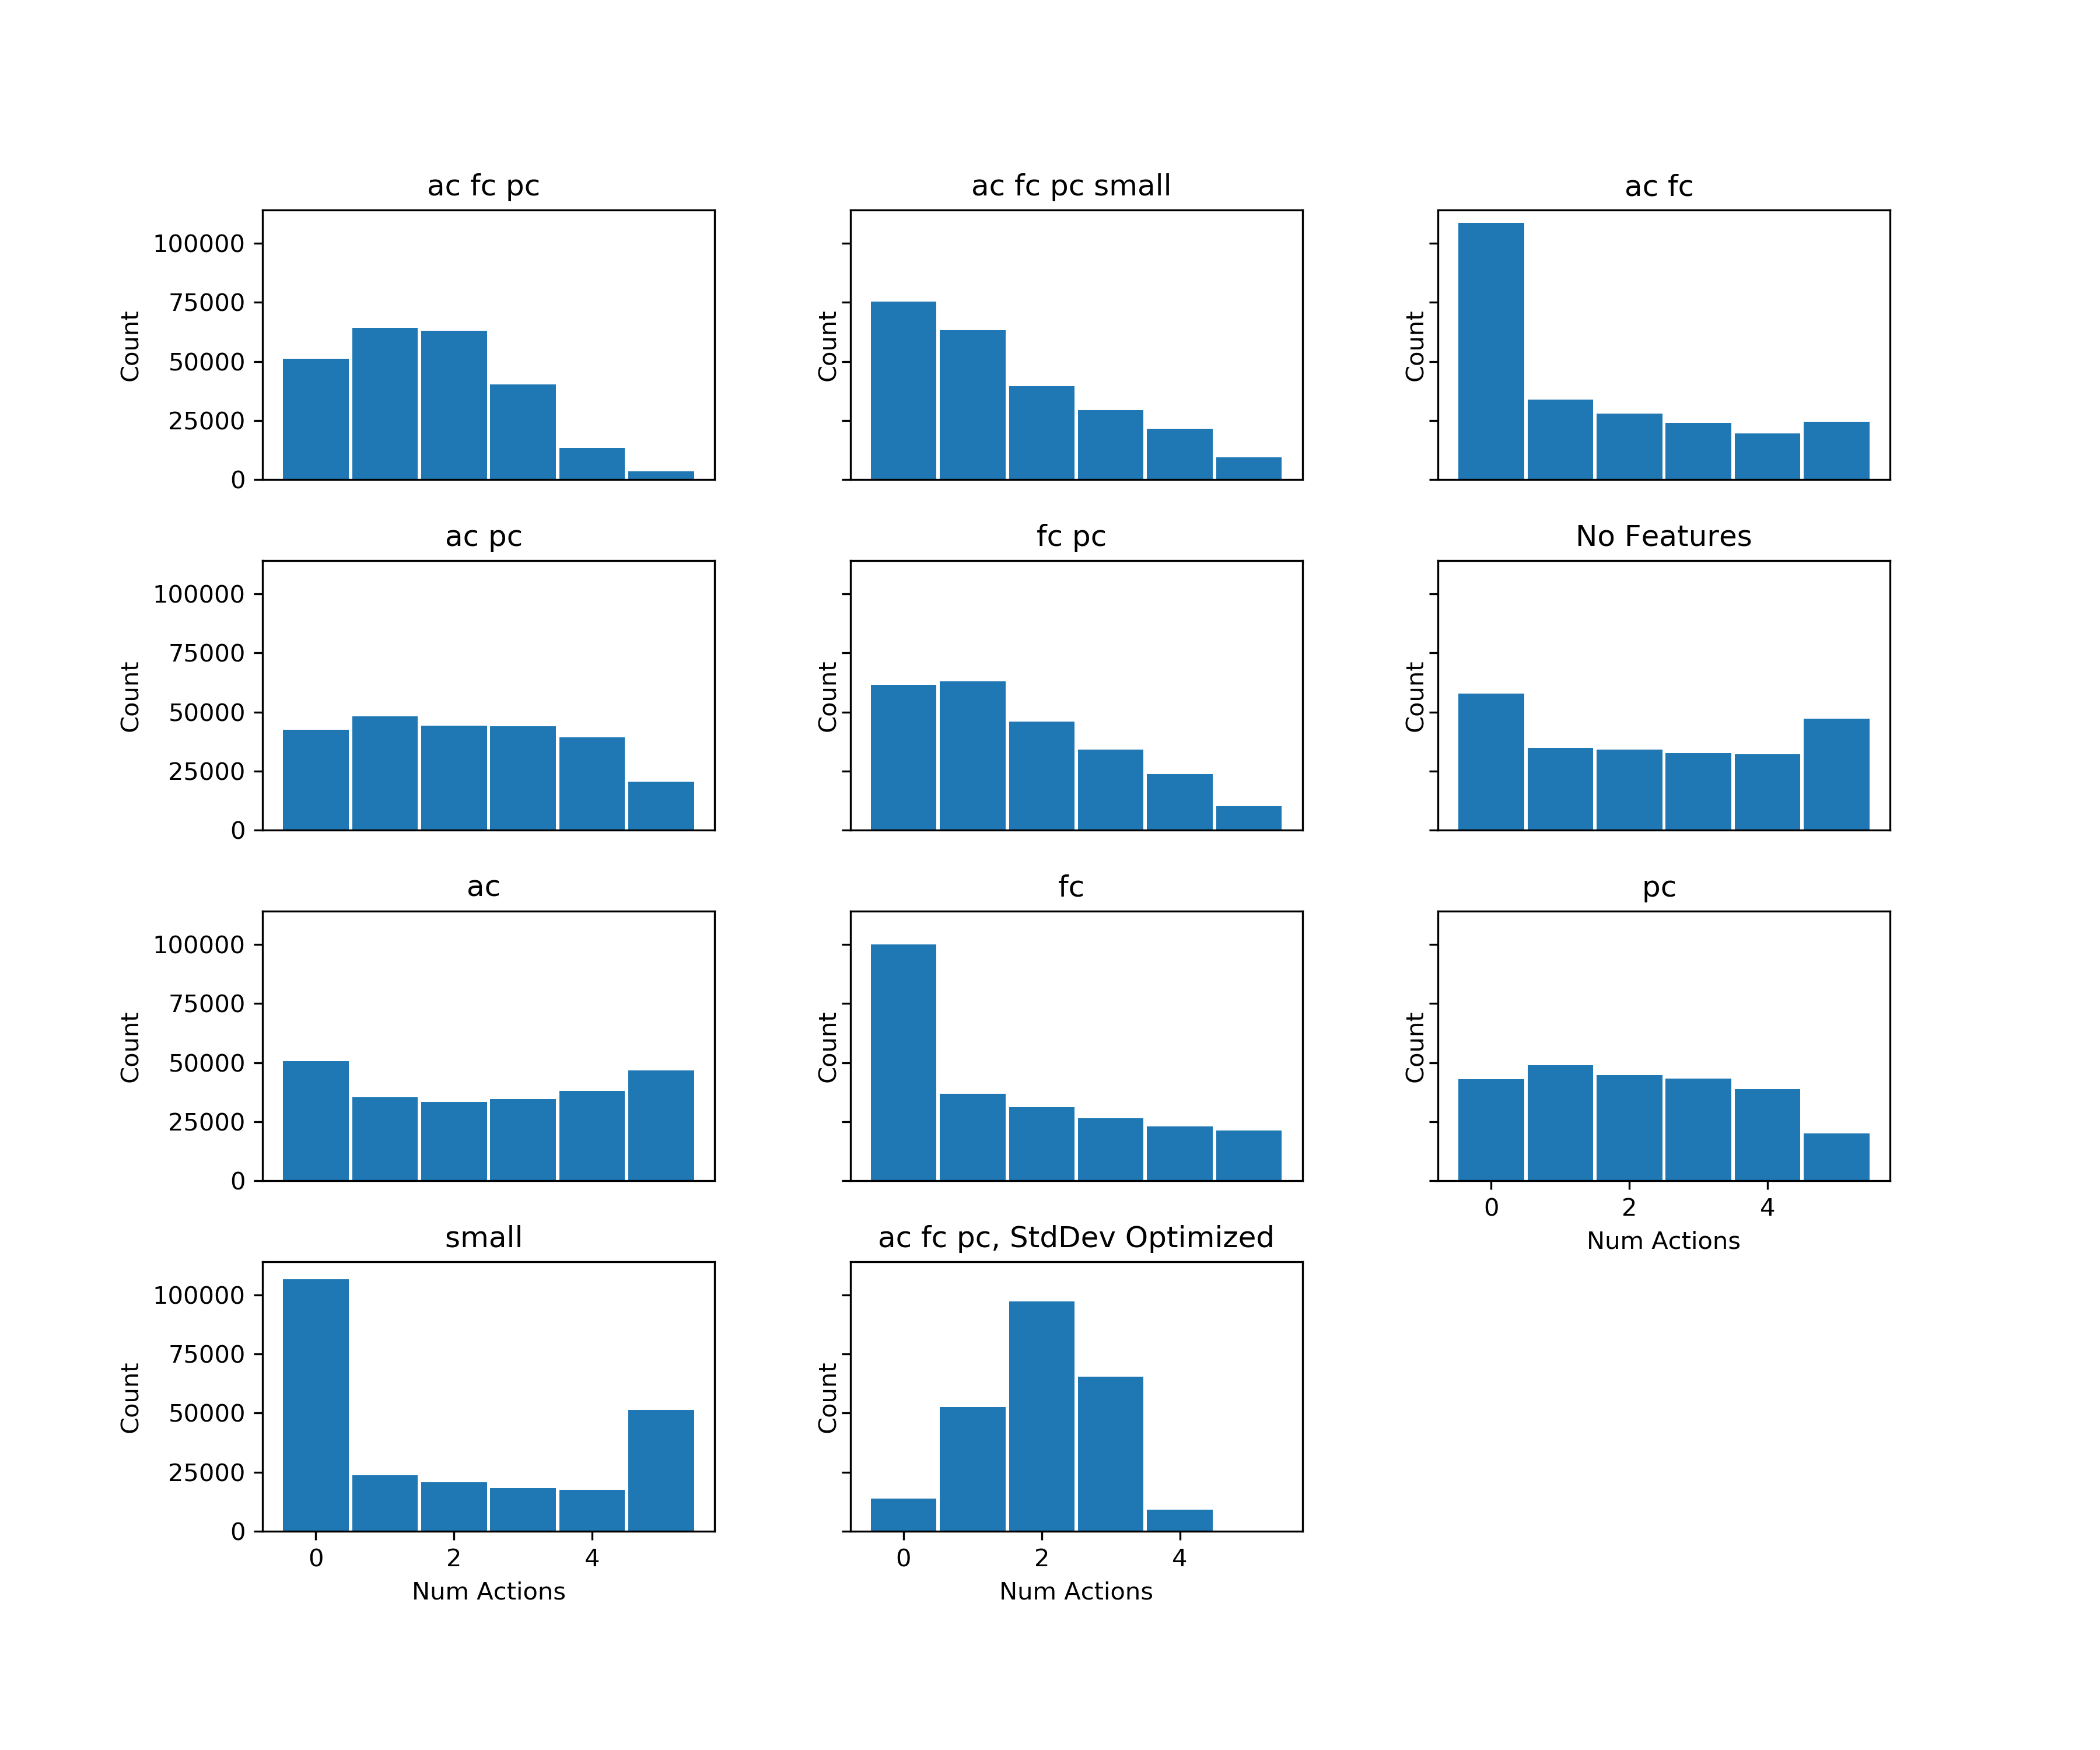
\includegraphics[width=1.5\textwidth,center]{figures/QM6test.png}%
	\caption{Number of Actions per Day across all Users in Testing Batches}
	\label{QM6test}
	\end{figure}

	\begin{figure}[H]
	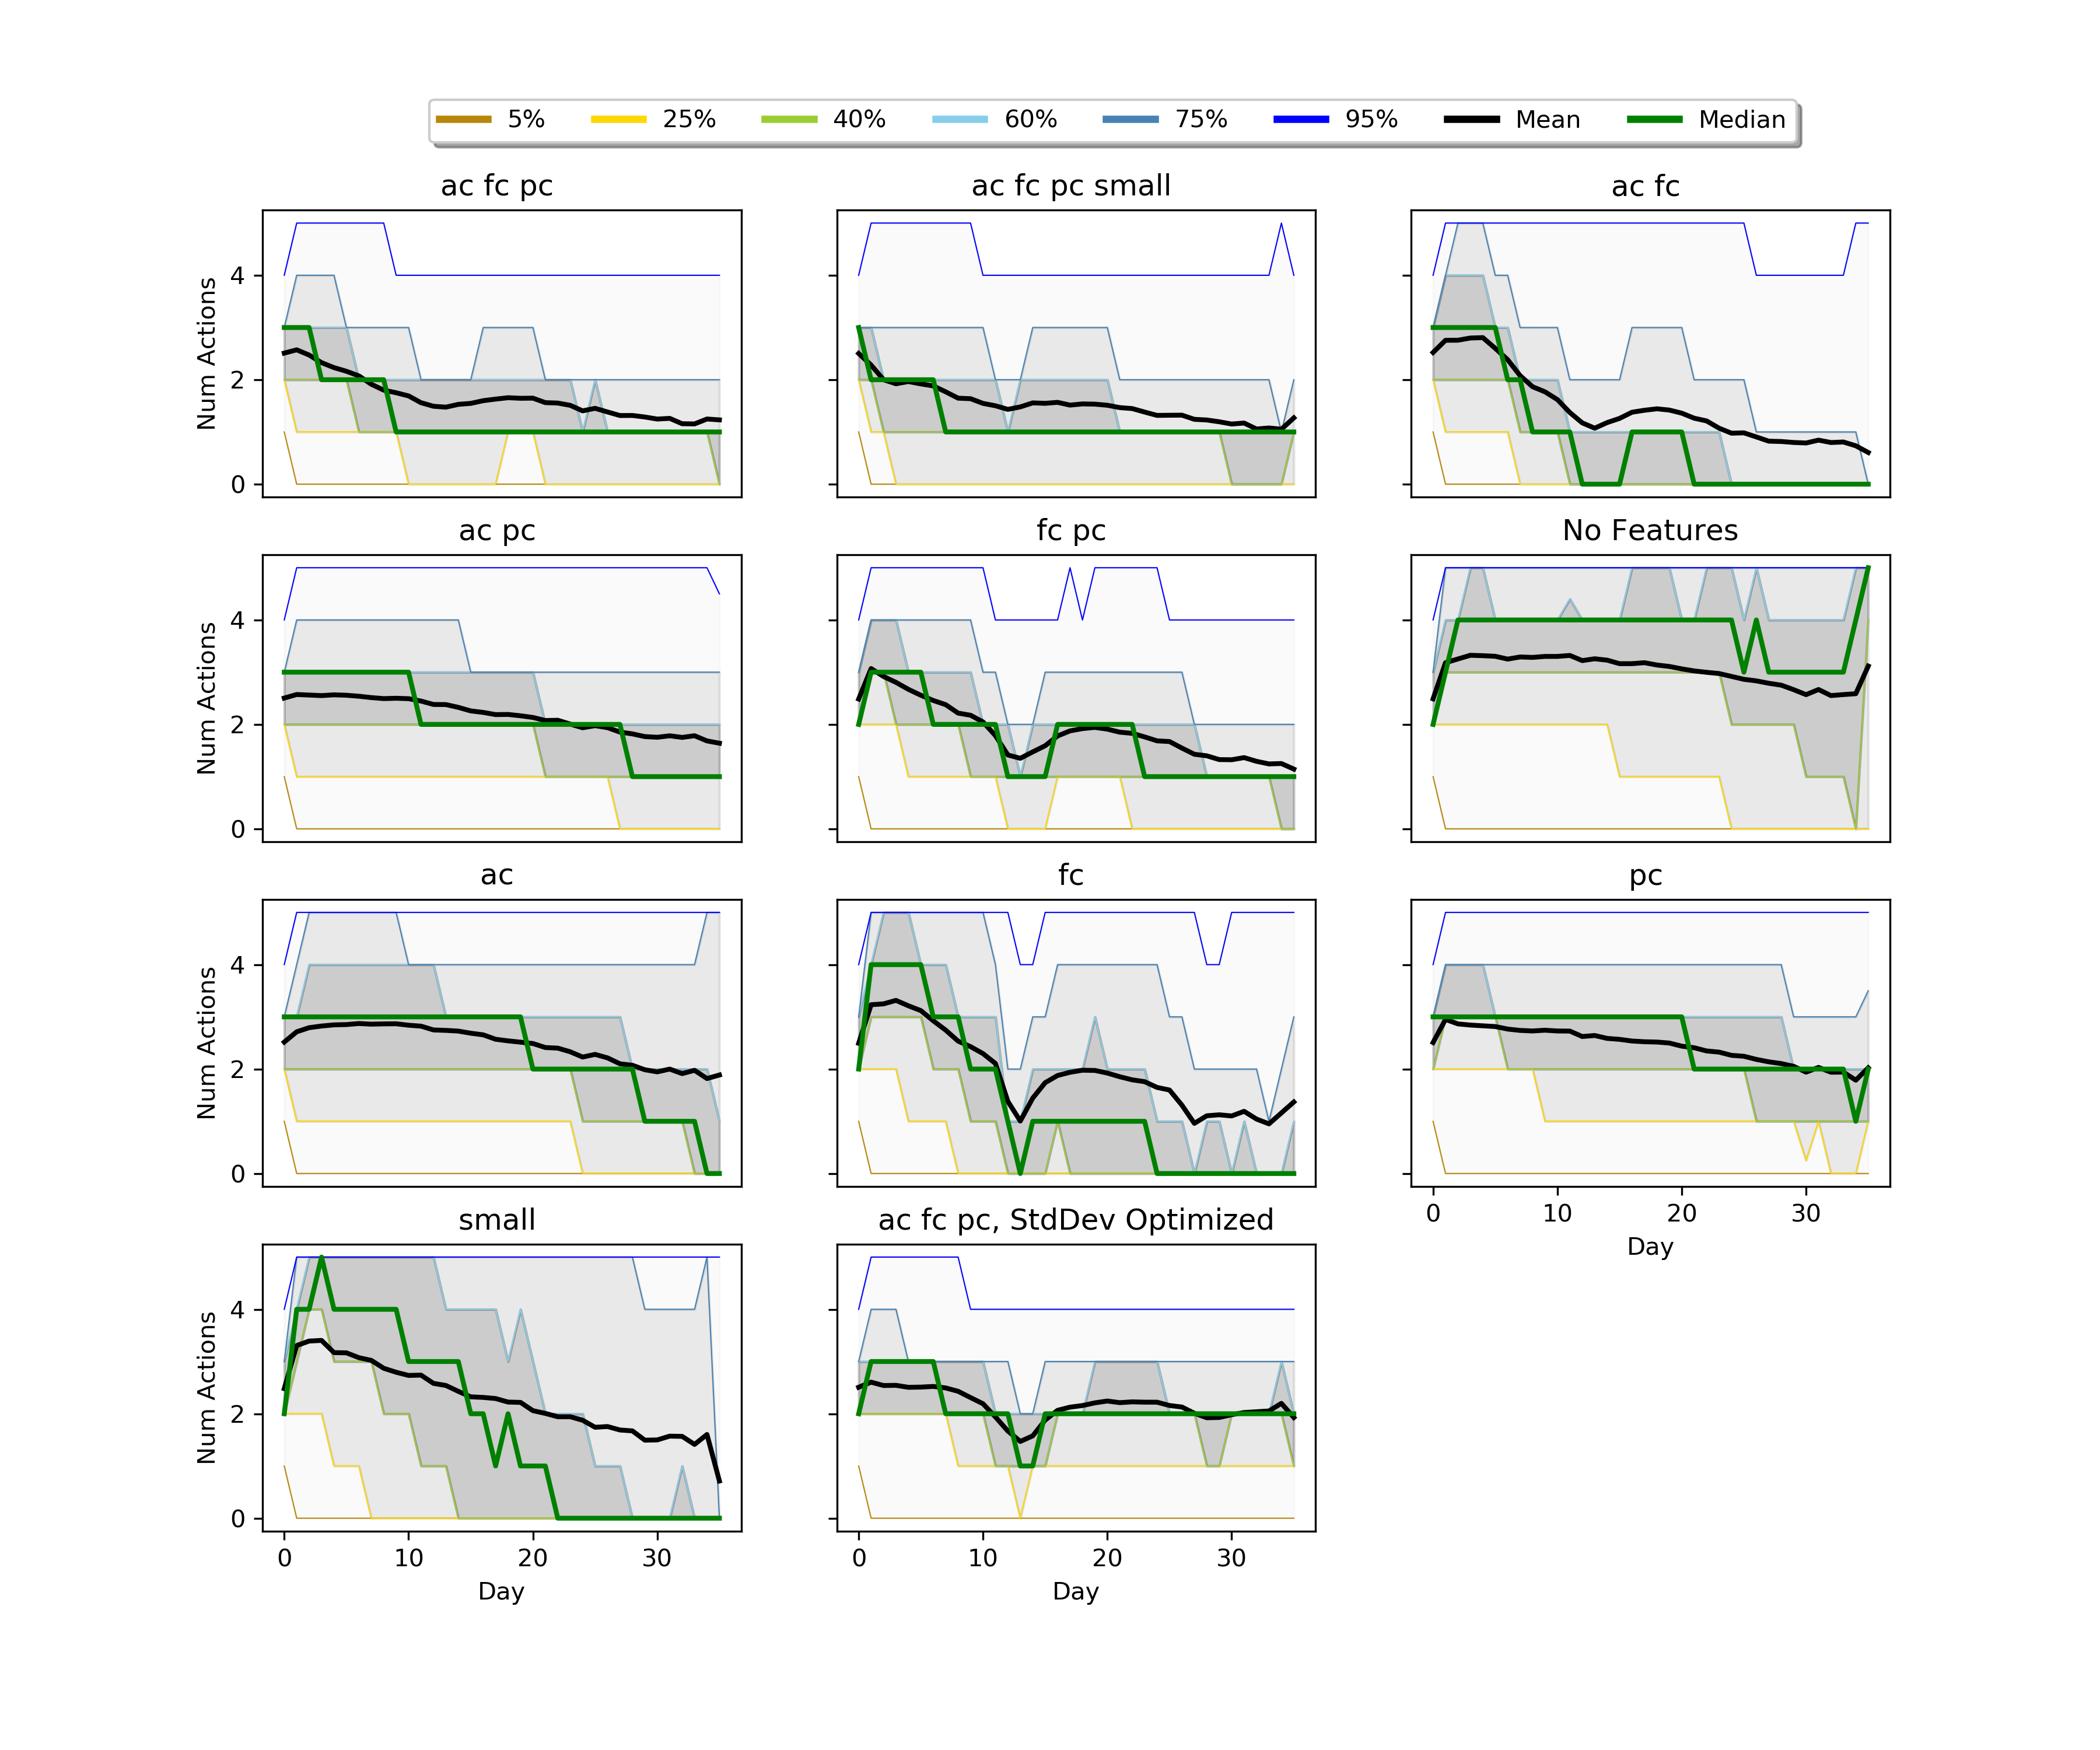
\includegraphics[width=1.5\textwidth,center]{figures/QM7train.png}%
	\caption{Number of Actions per Day for Users in Optimal Training Batches}
	\label{QM7train}
	\end{figure}

	\begin{figure}[H]
	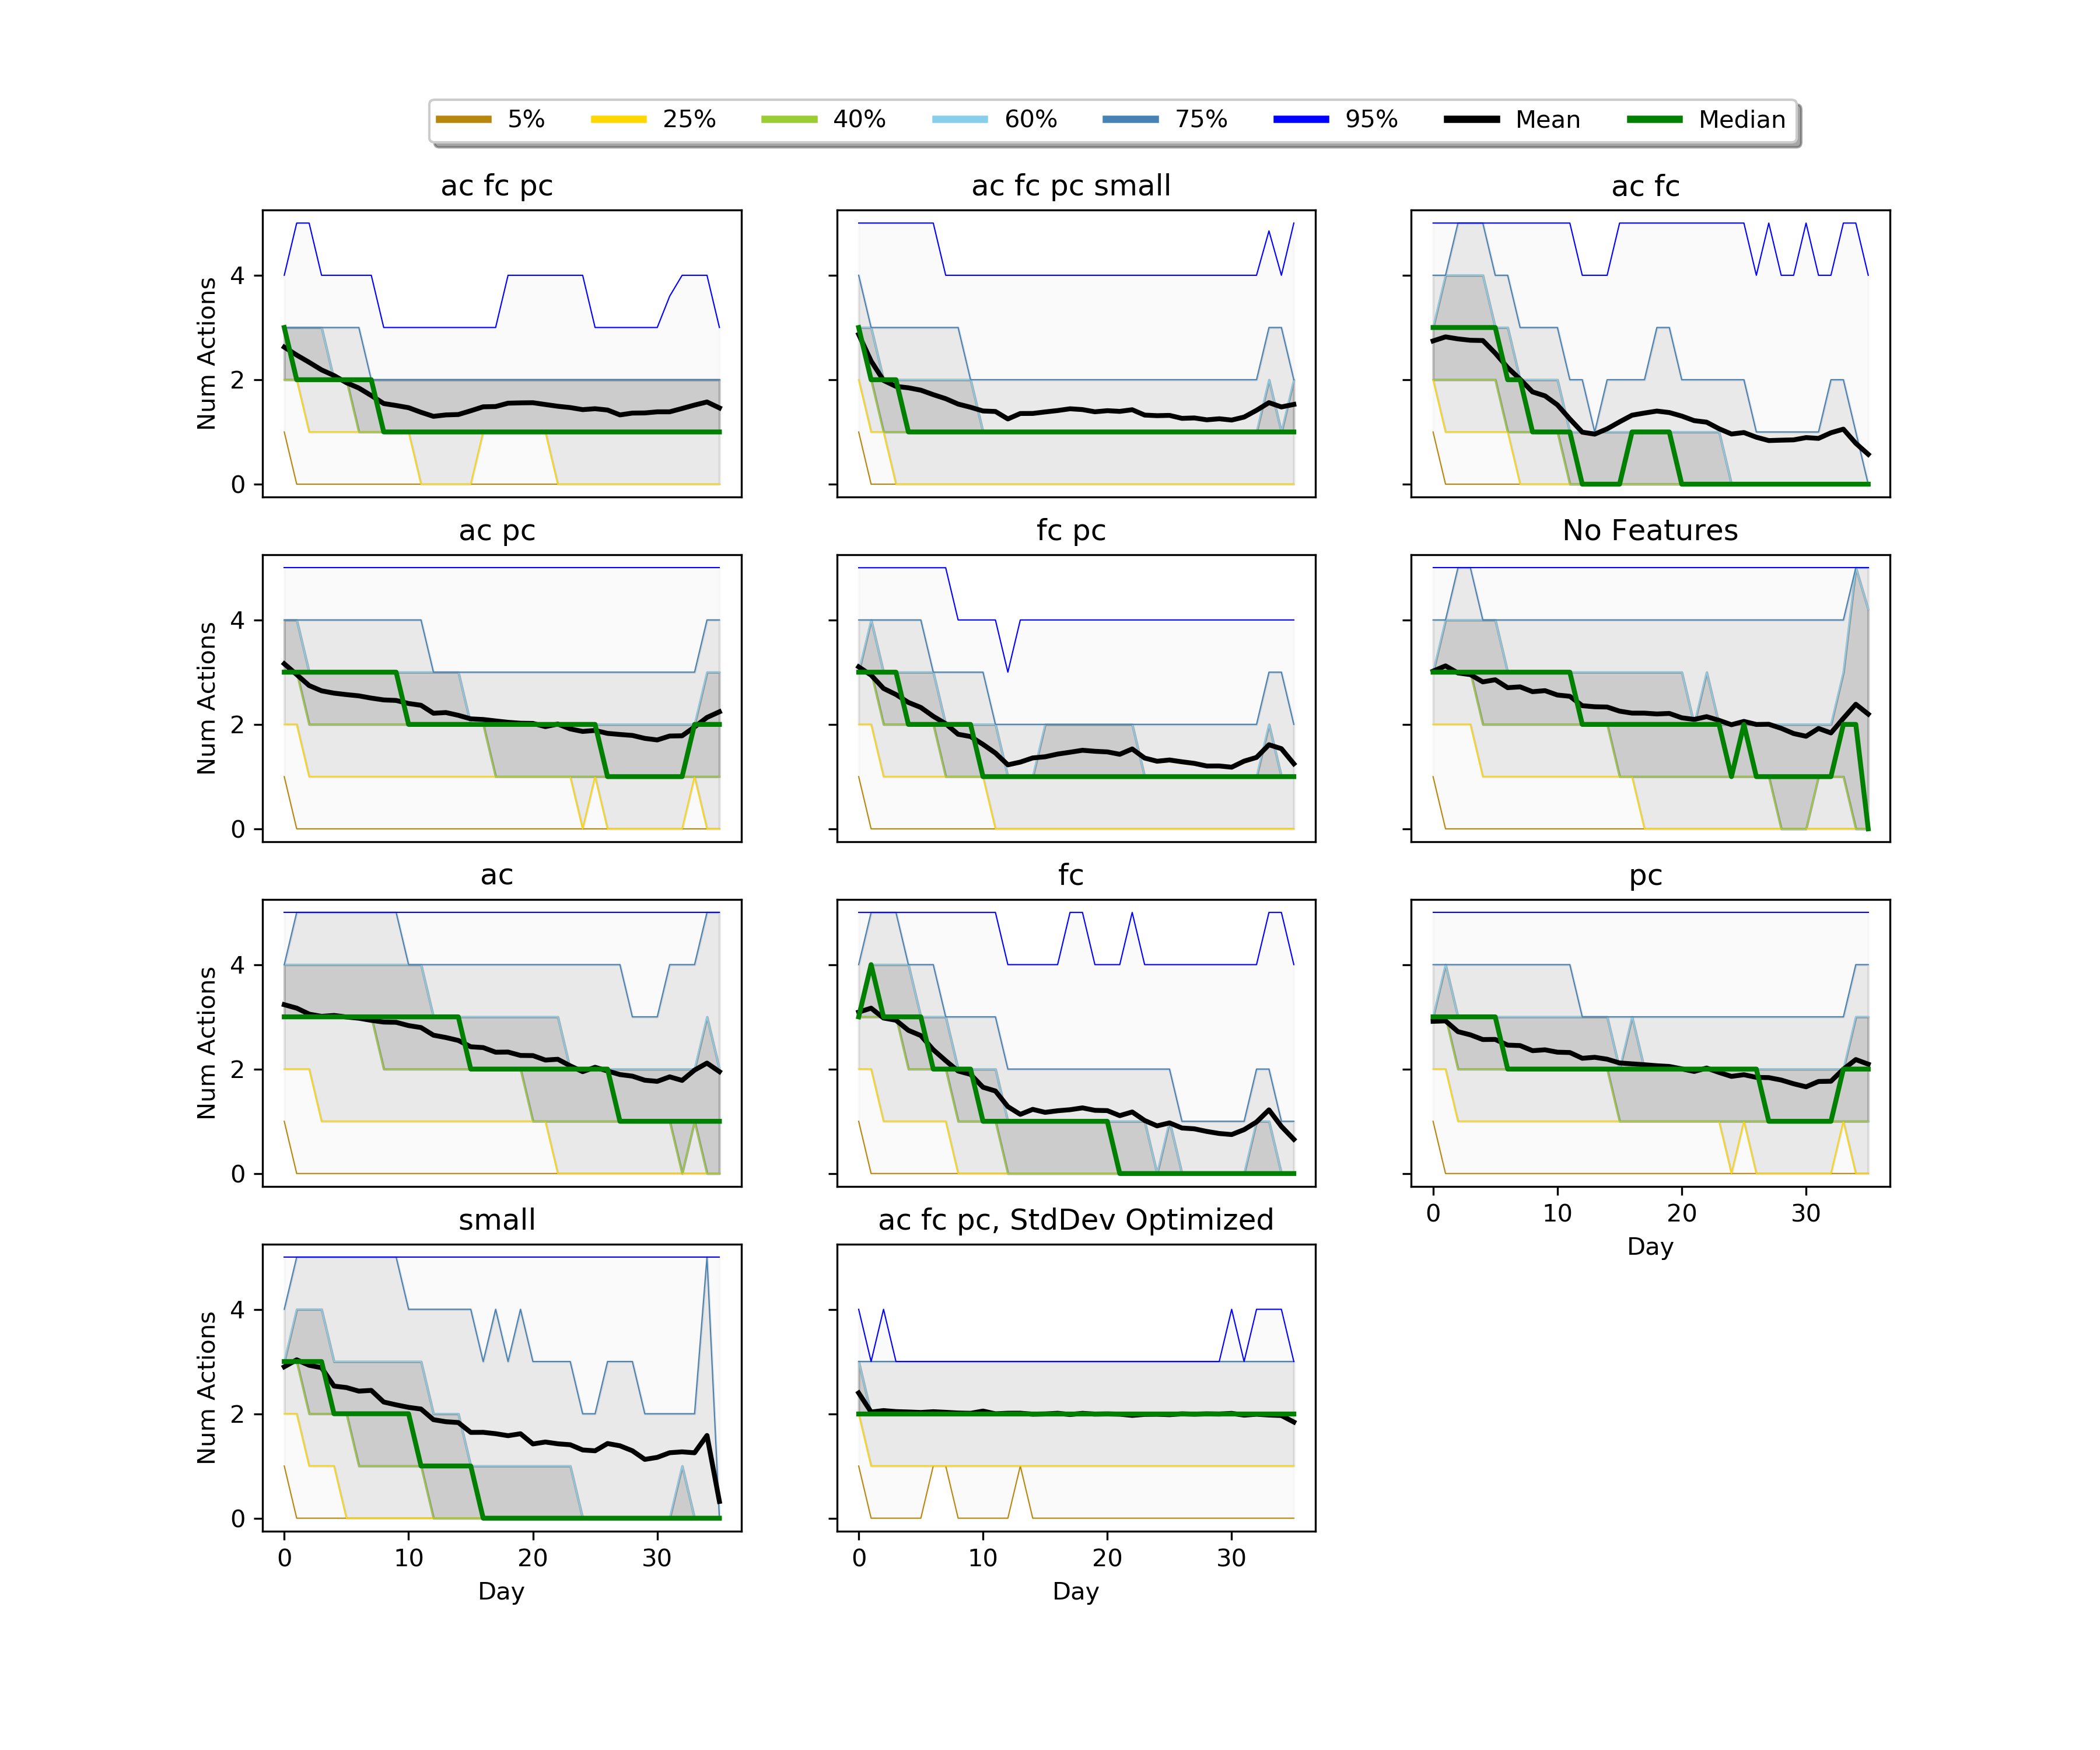
\includegraphics[width=1.5\textwidth,center]{figures/QM7test.png}%
	\caption{Number of Actions per Day for Users in Testing Batches}
	\label{QM7test}
	\end{figure}

	\begin{figure}[H]
	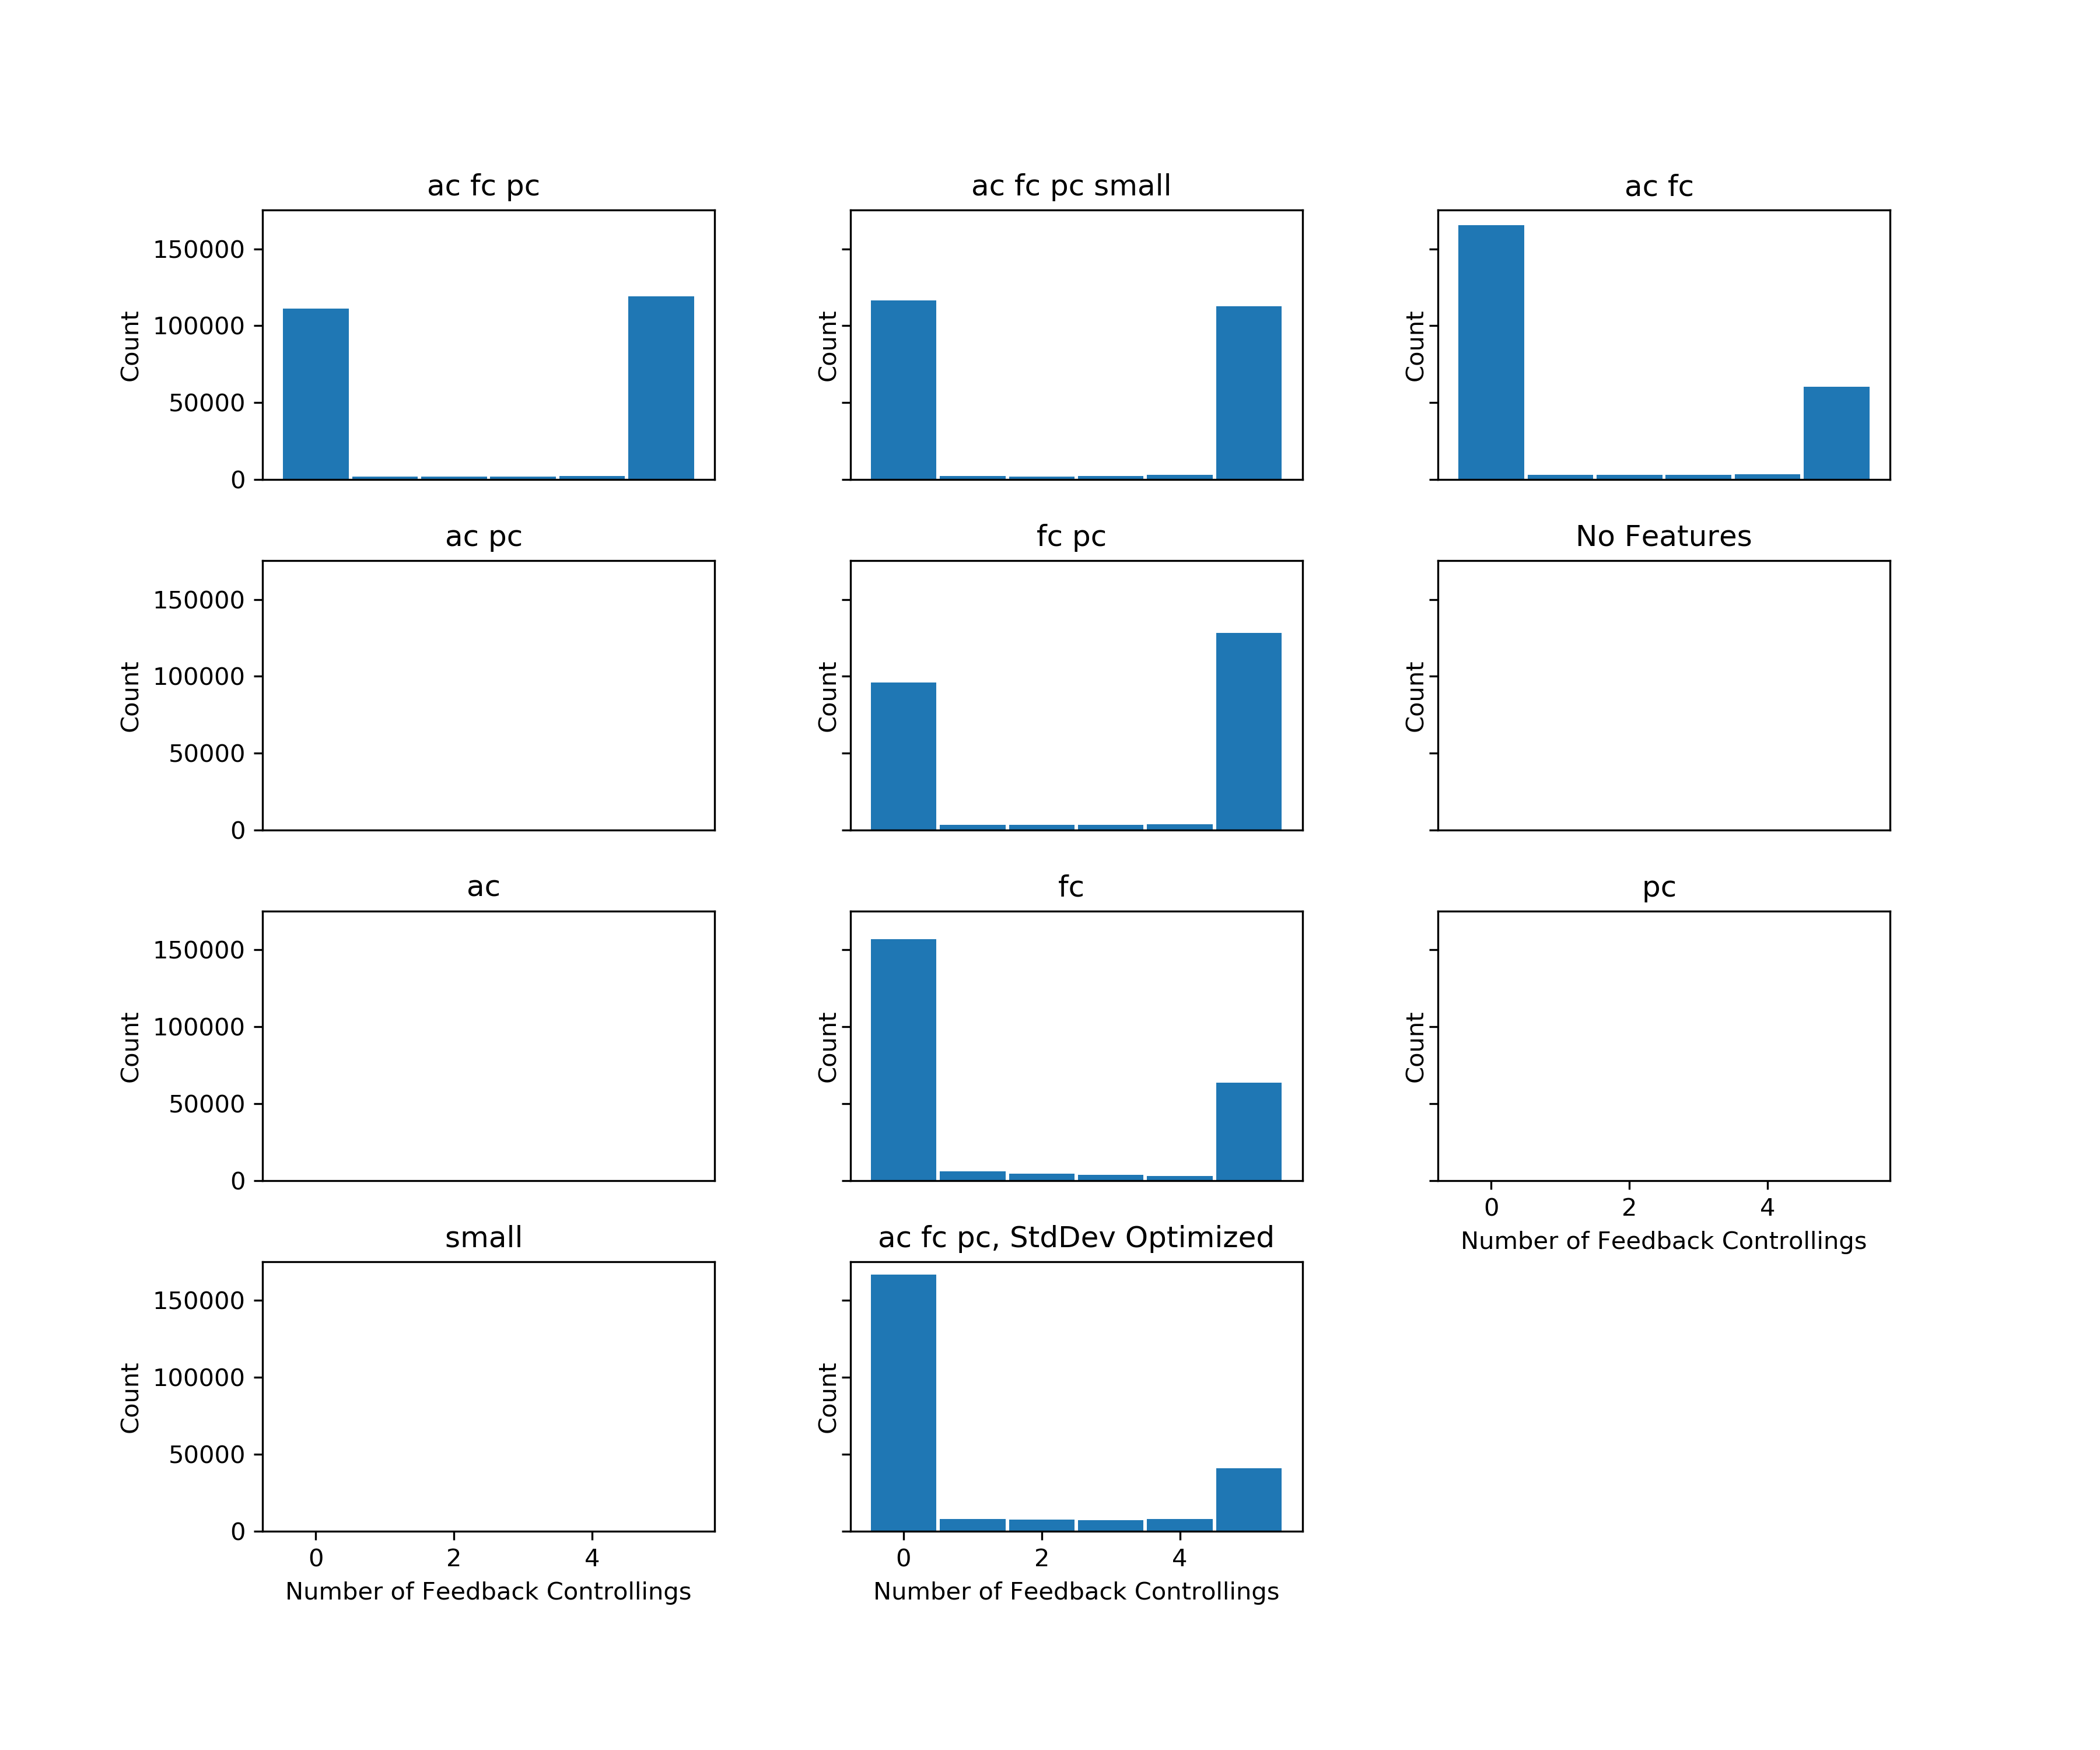
\includegraphics[width=1.5\textwidth,center]{figures/QM8train.png}%
	\caption{Number of Feedback Controllings per Day across all Users in Optimal Training Batches}
	\label{QM8train}
	\end{figure}

	\begin{figure}[H]
	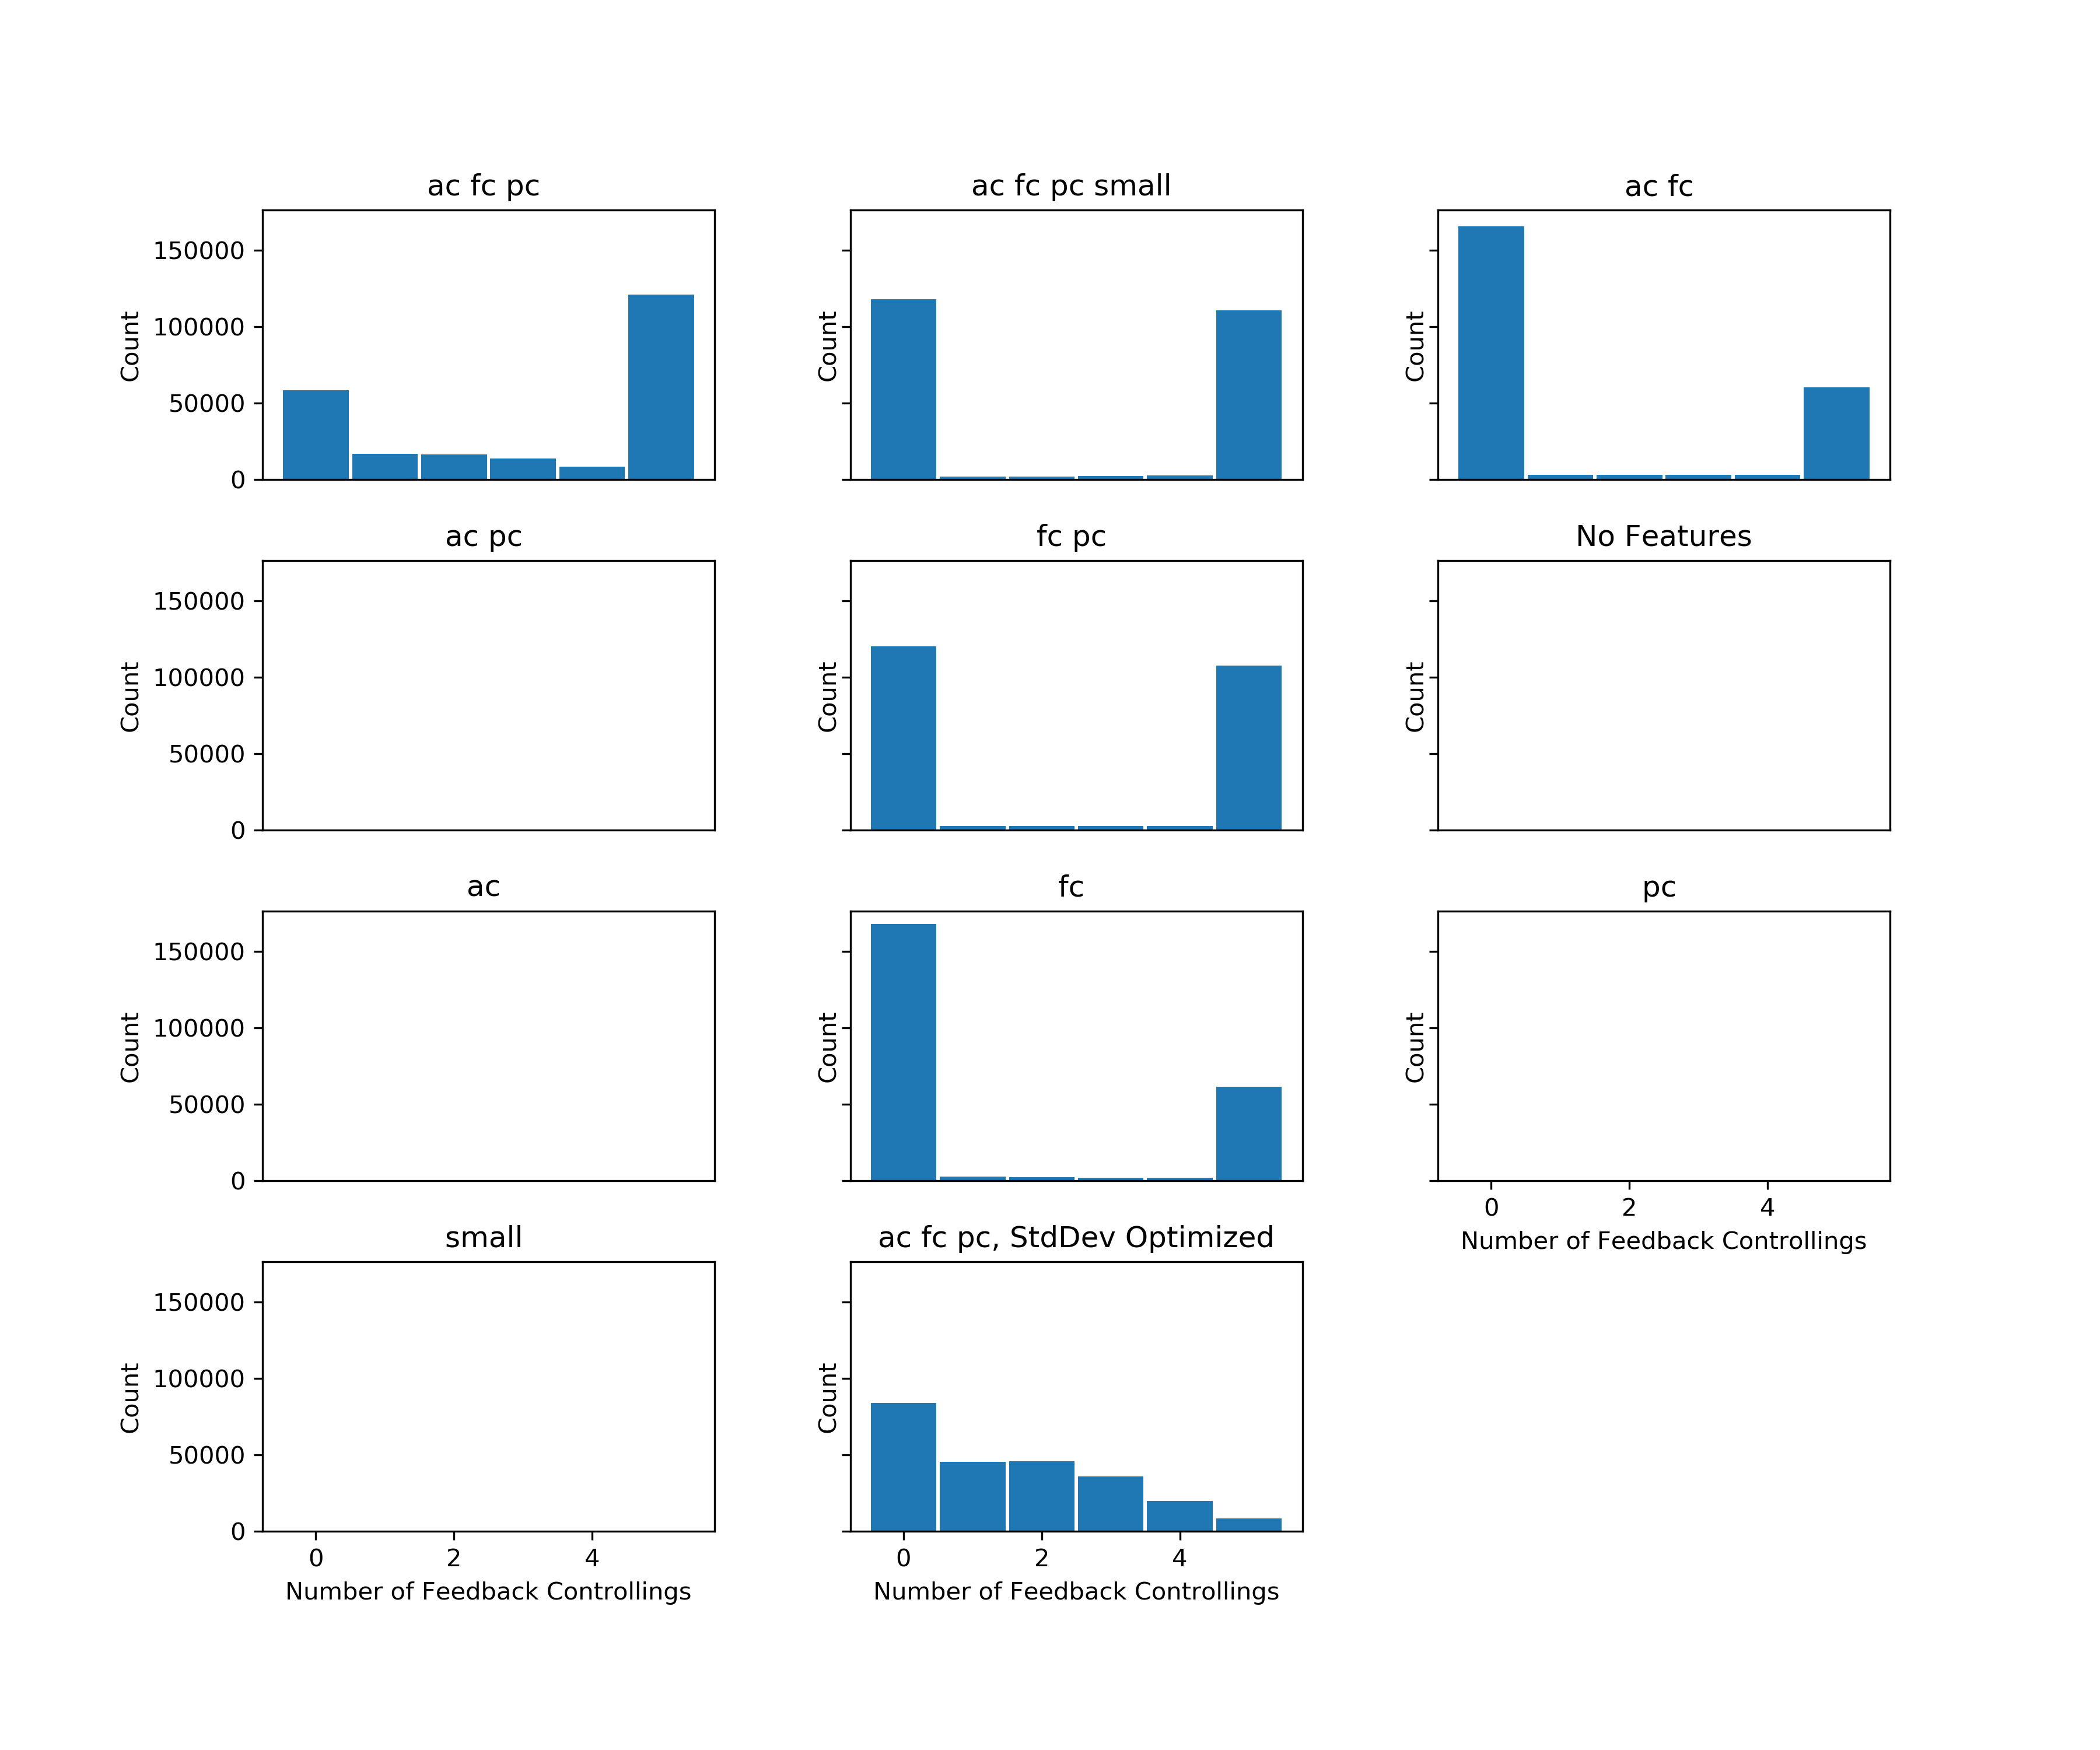
\includegraphics[width=1.5\textwidth,center]{figures/QM8test.png}%
	\caption{Number of Feedback Controllings per Day across all Users in Testing Batches}
	\label{QM8test}
	\end{figure}

	\begin{figure}[H]
	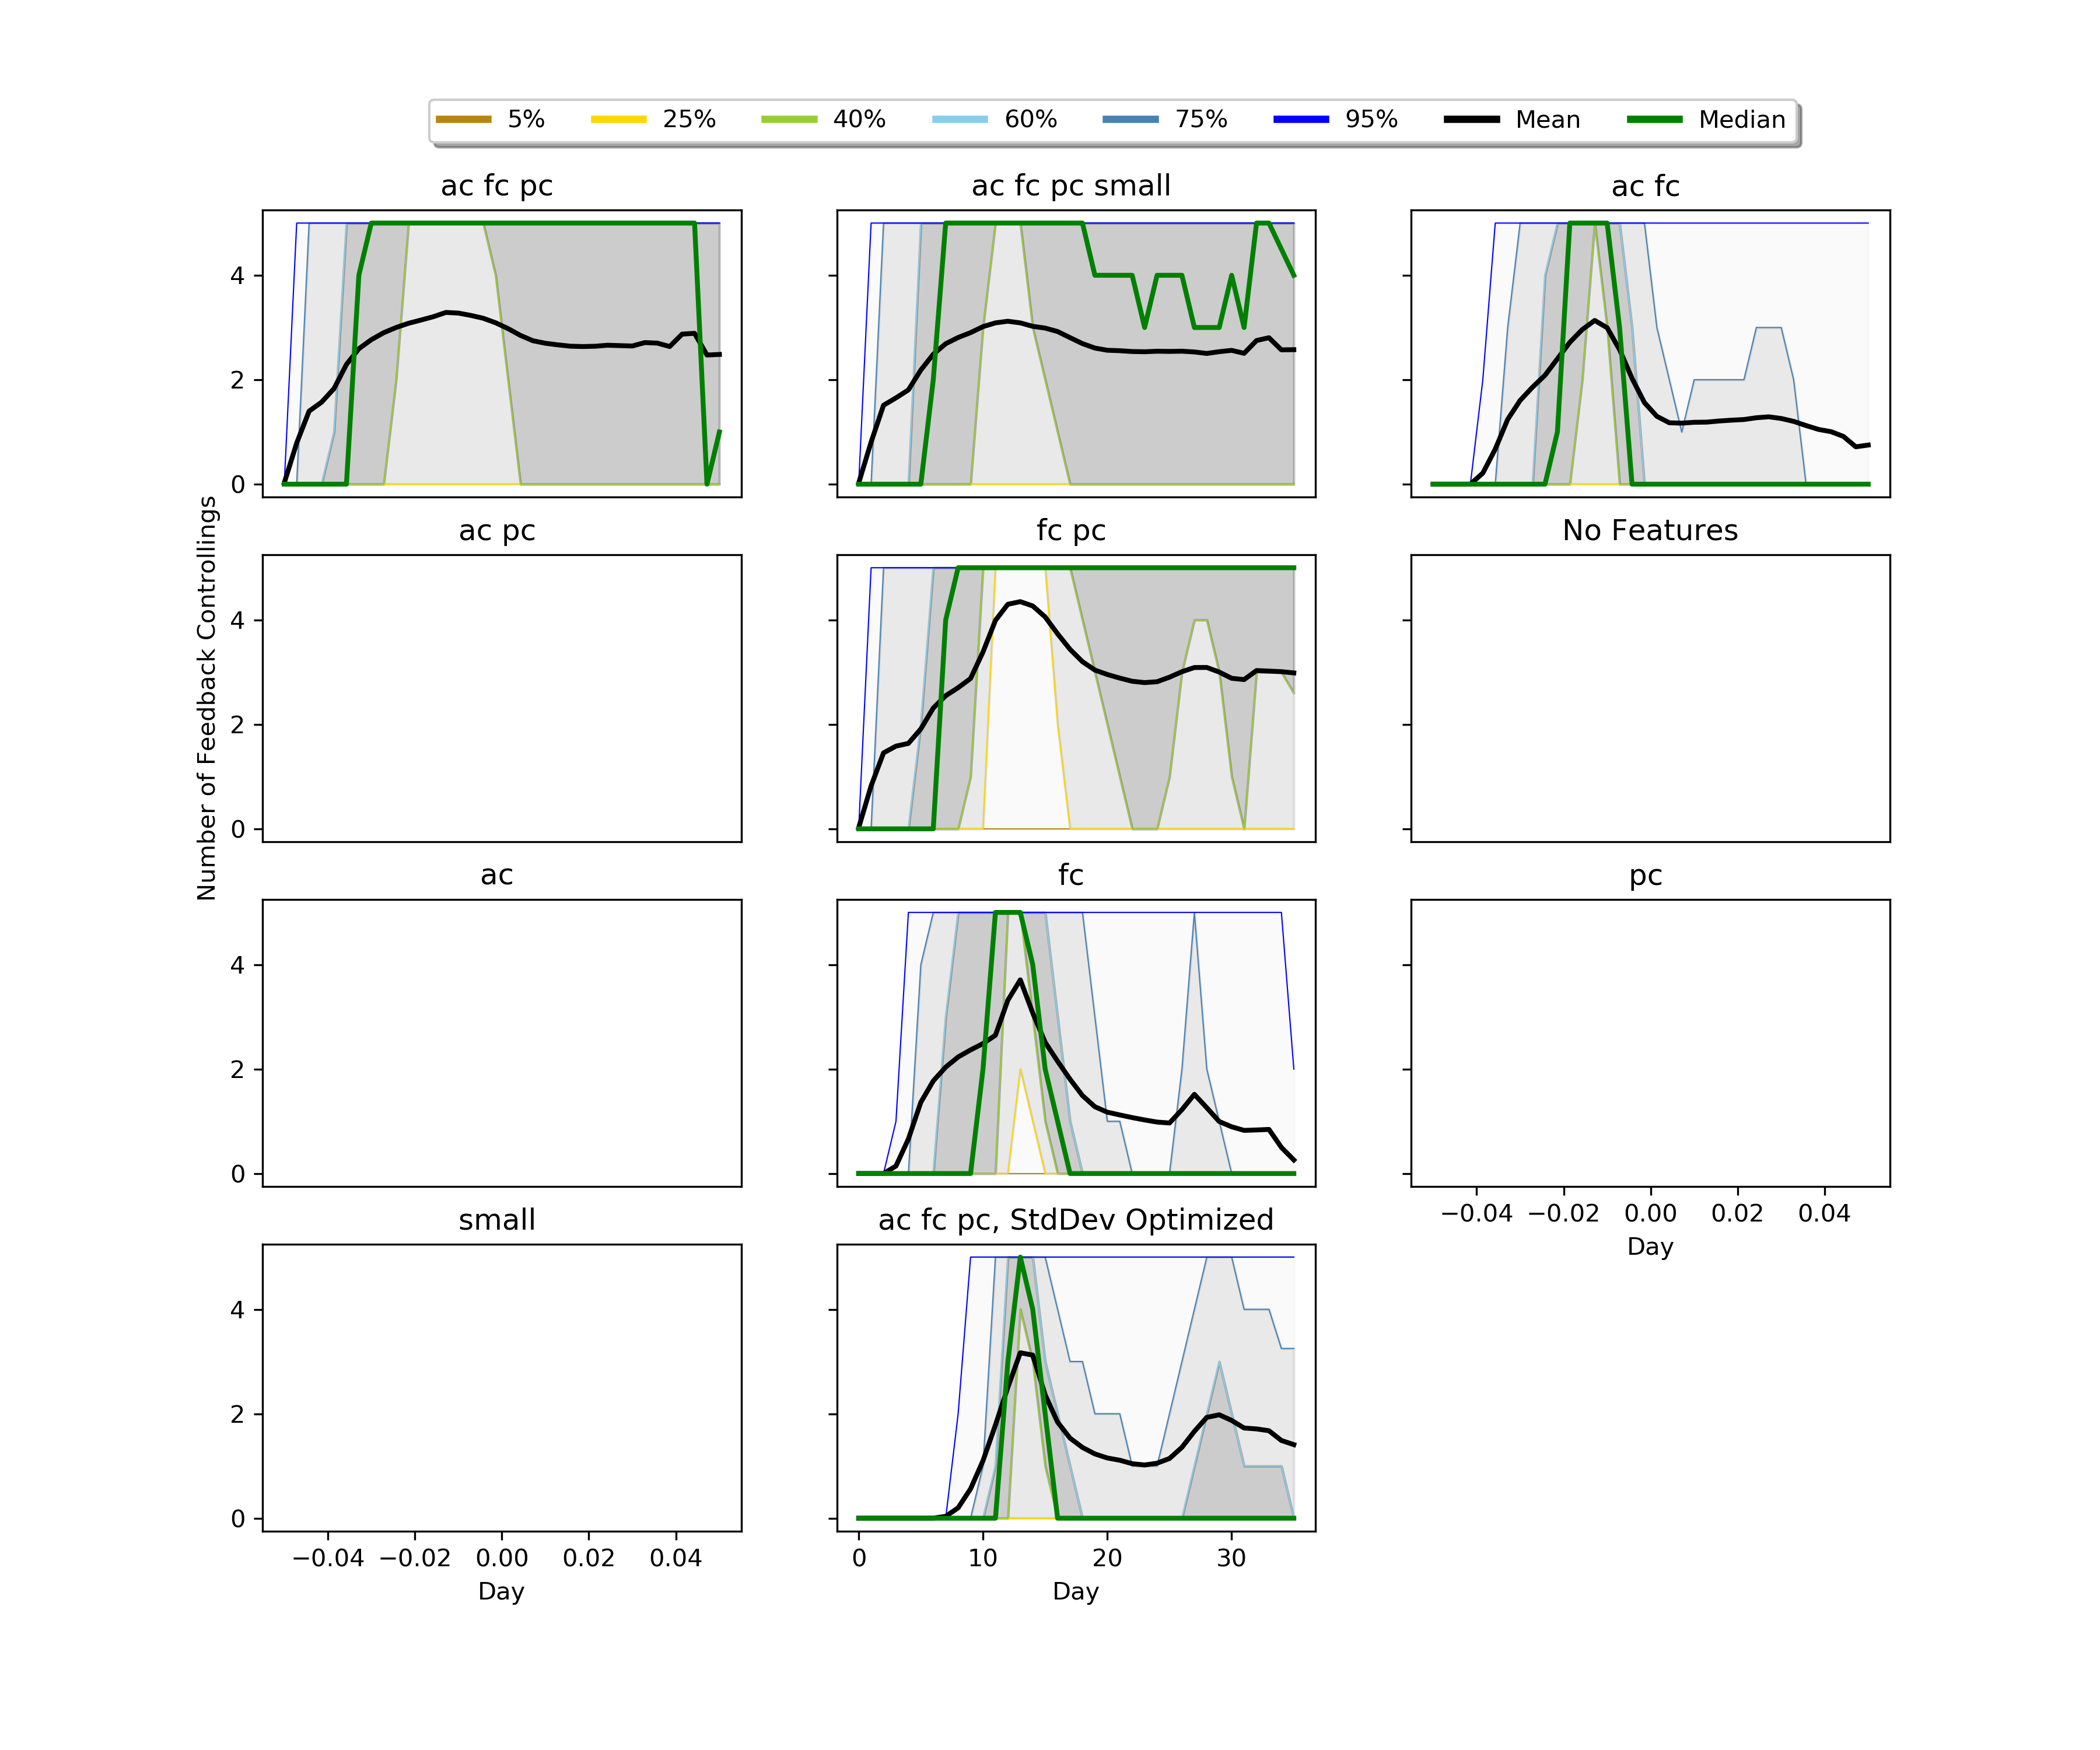
\includegraphics[width=1.5\textwidth,center]{figures/QM9train.png}%
	\caption{Number of Feedback Controllings per Day for Users in Optimal Training Batches}
	\label{QM9train}
	\end{figure}

	\begin{figure}[H]
	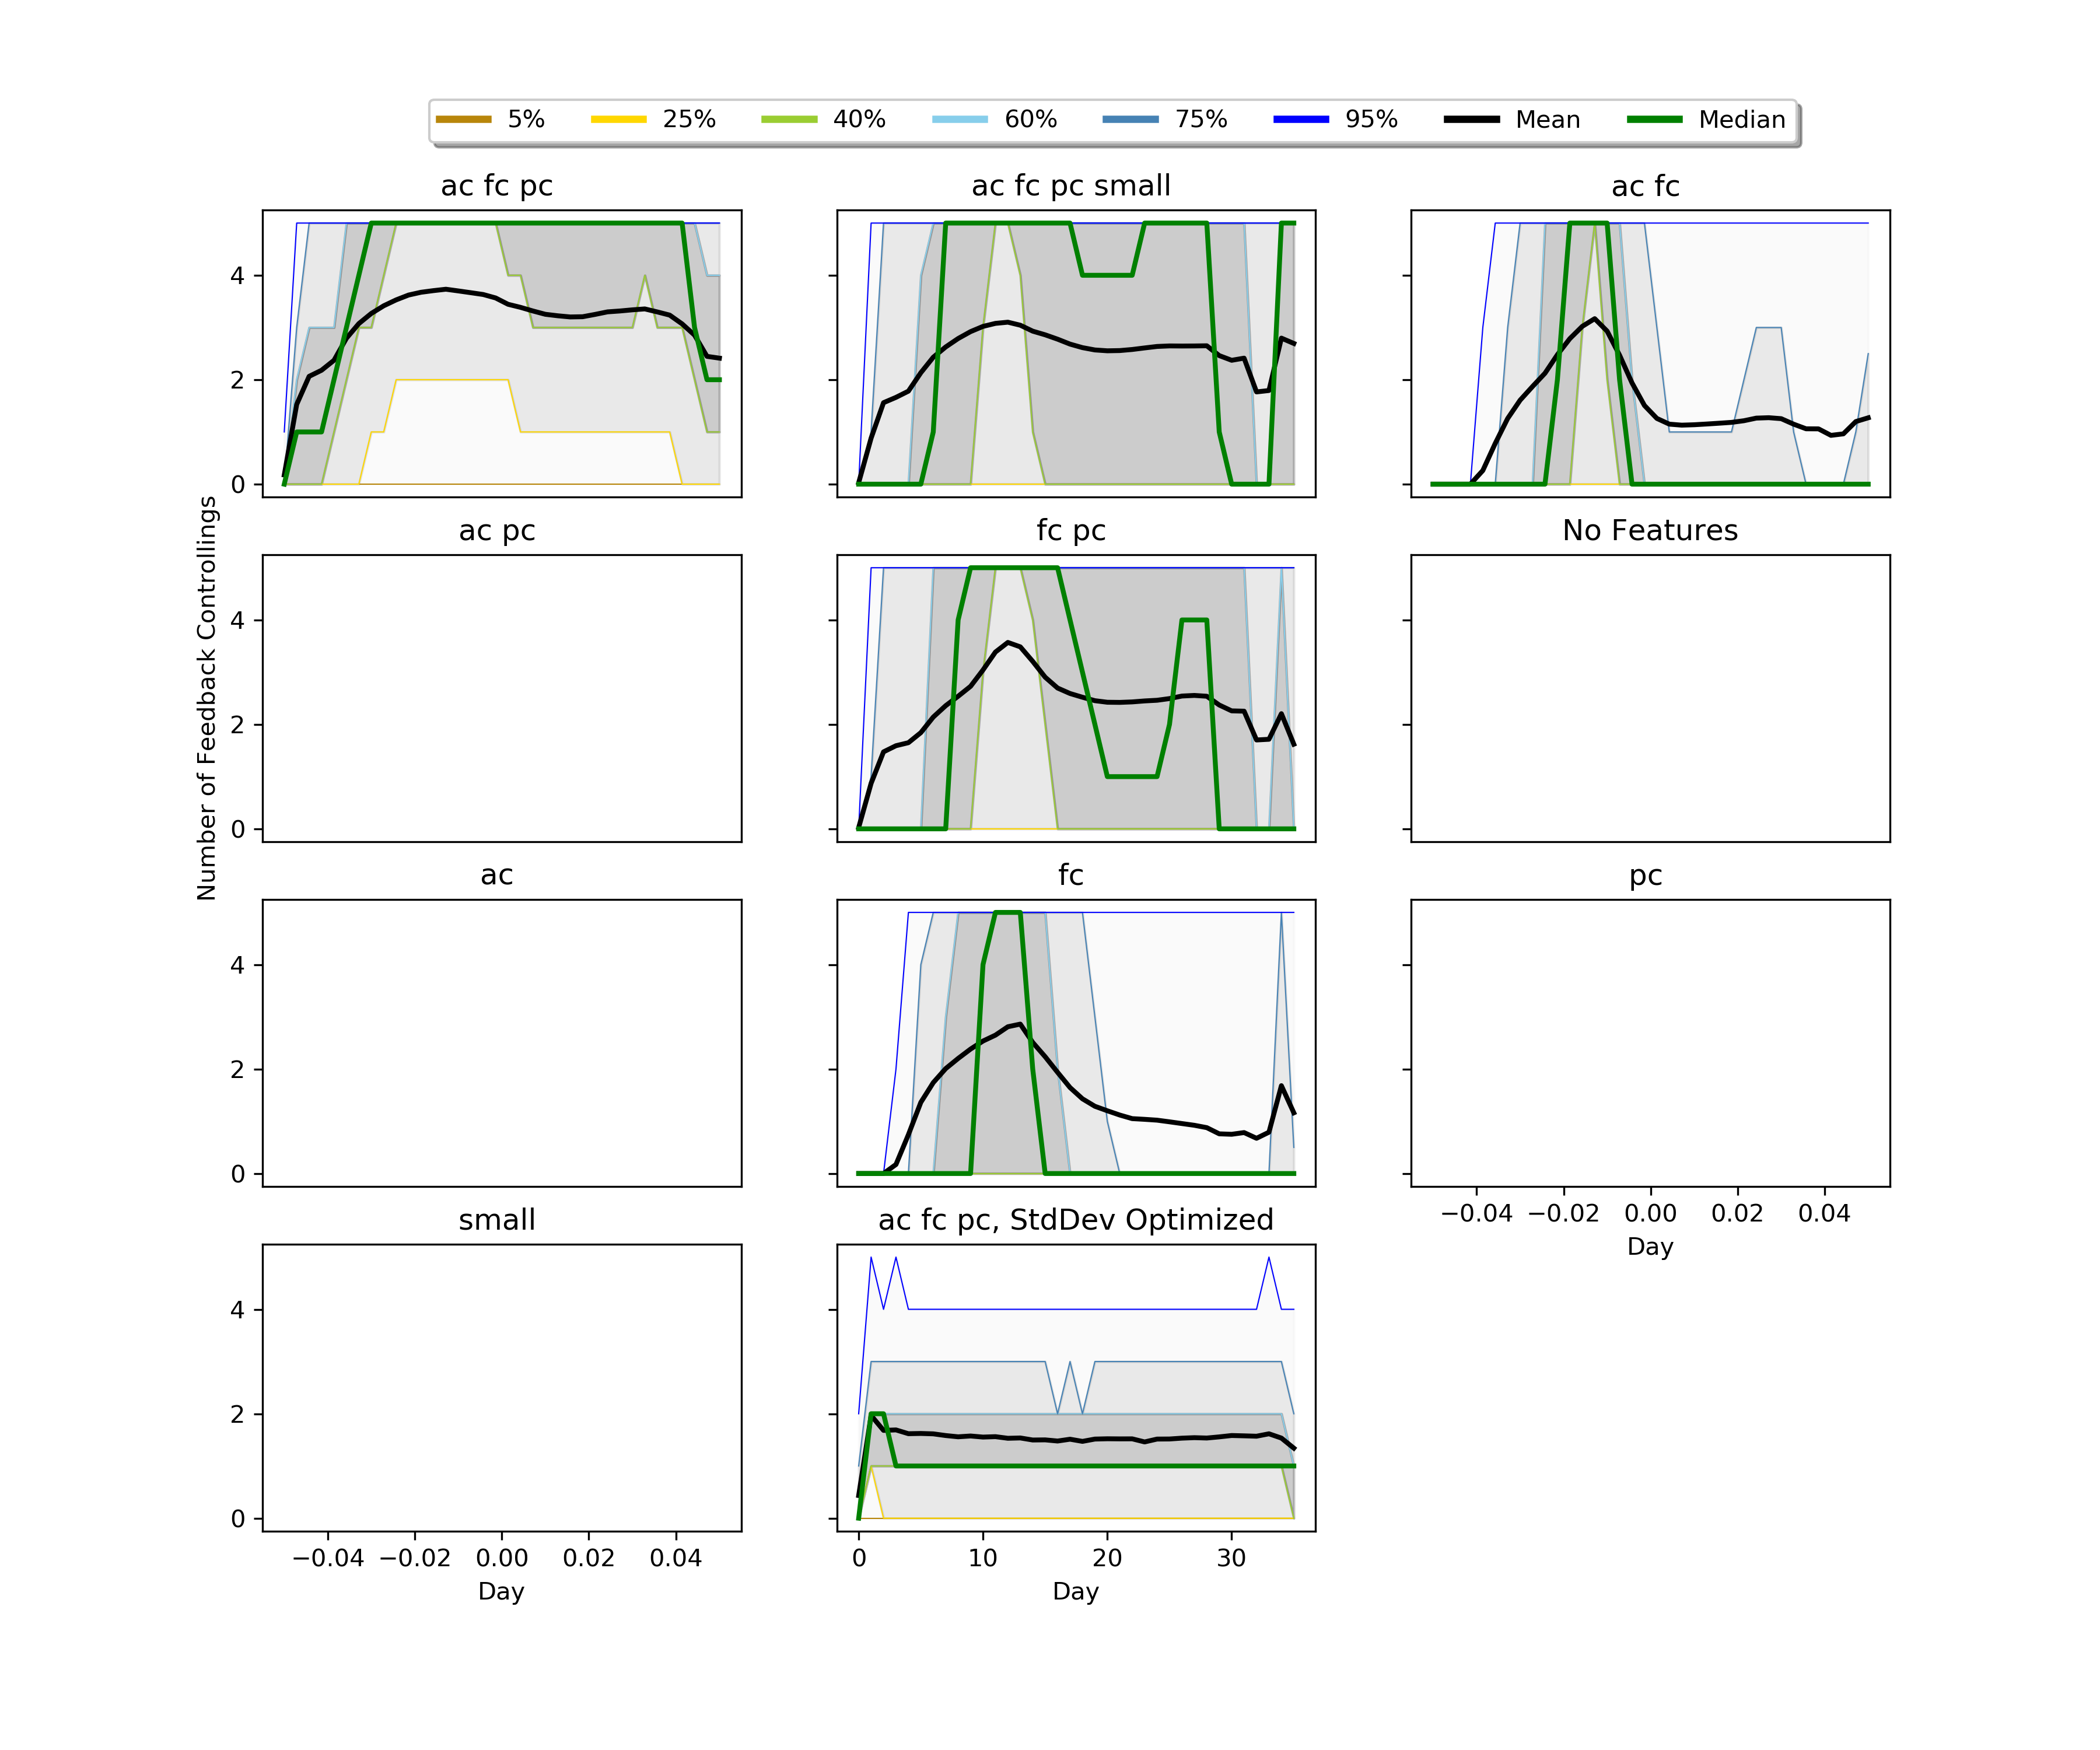
\includegraphics[width=1.5\textwidth,center]{figures/QM9test.png}%
	\caption{Number of Feedback Controllings per Day for Users in Testing Batches}
	\label{QM9test}
	\end{figure}

	\begin{figure}[H]
	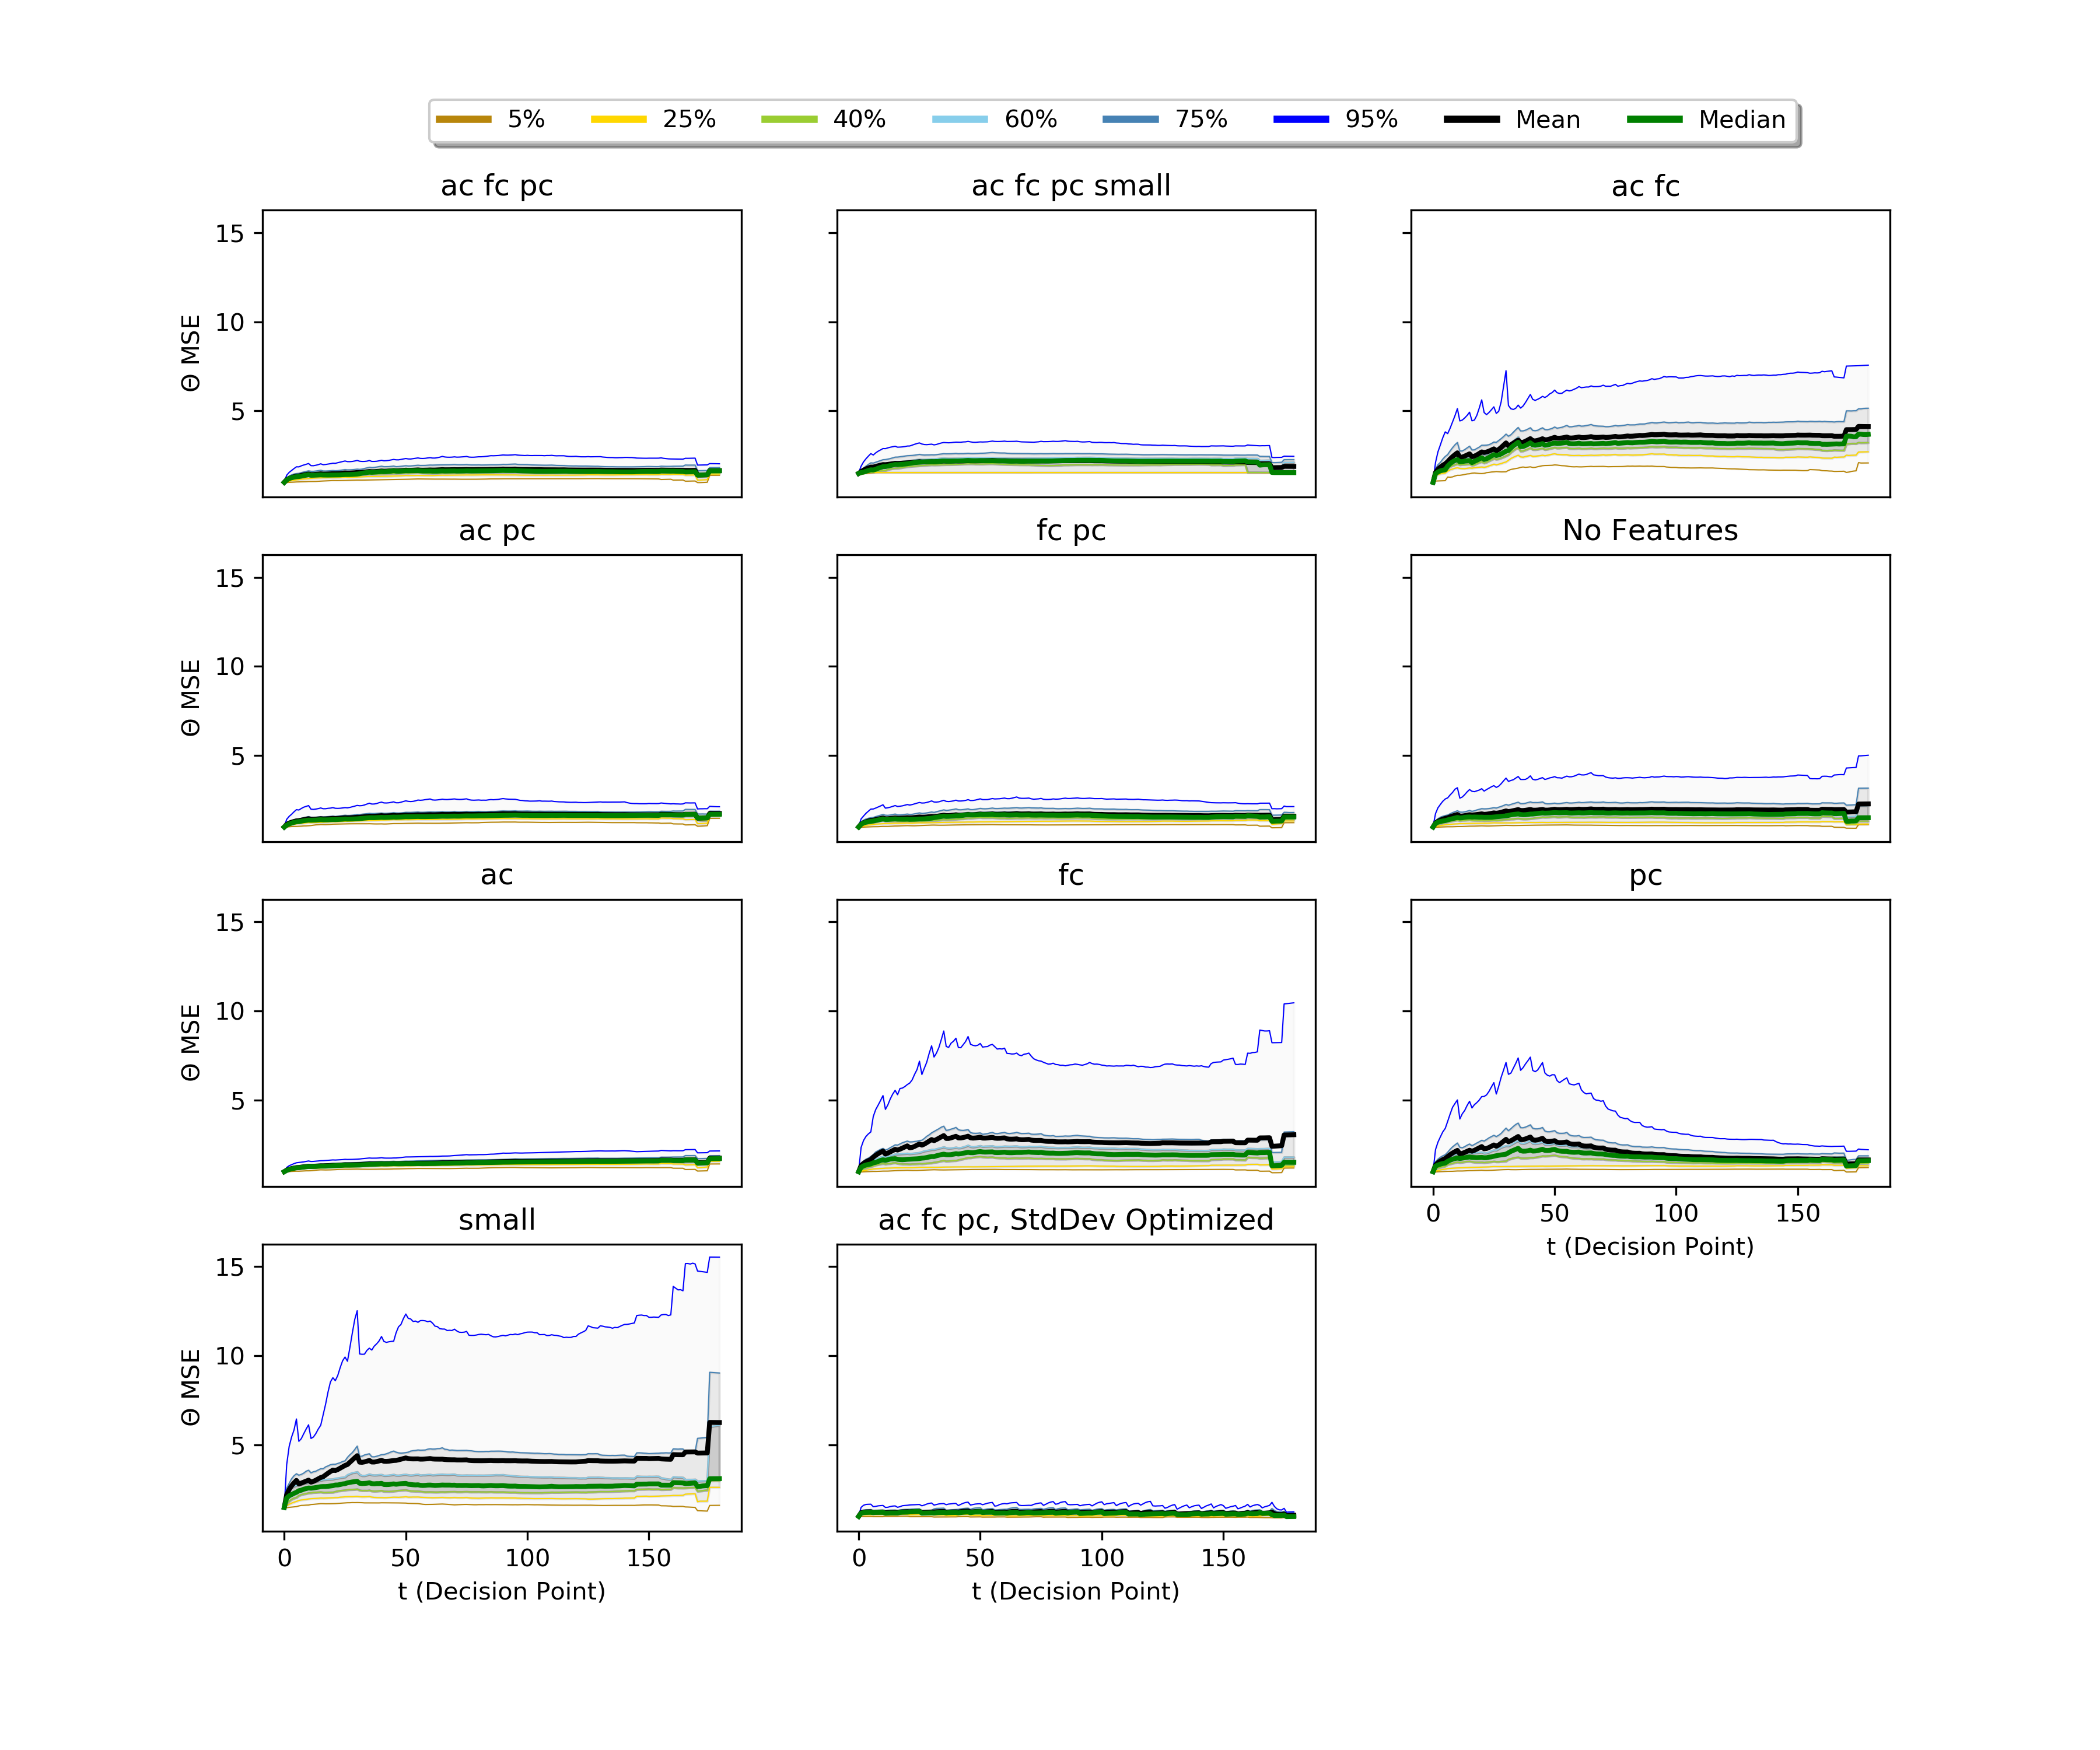
\includegraphics[width=1.5\textwidth,center]{figures/QM11train.png}%
	\caption{Bandit Model $\Theta$ MSE for All Users in Optimal Training Batches}
	\label{QM11train}
	\end{figure}

	\begin{figure}[H]
	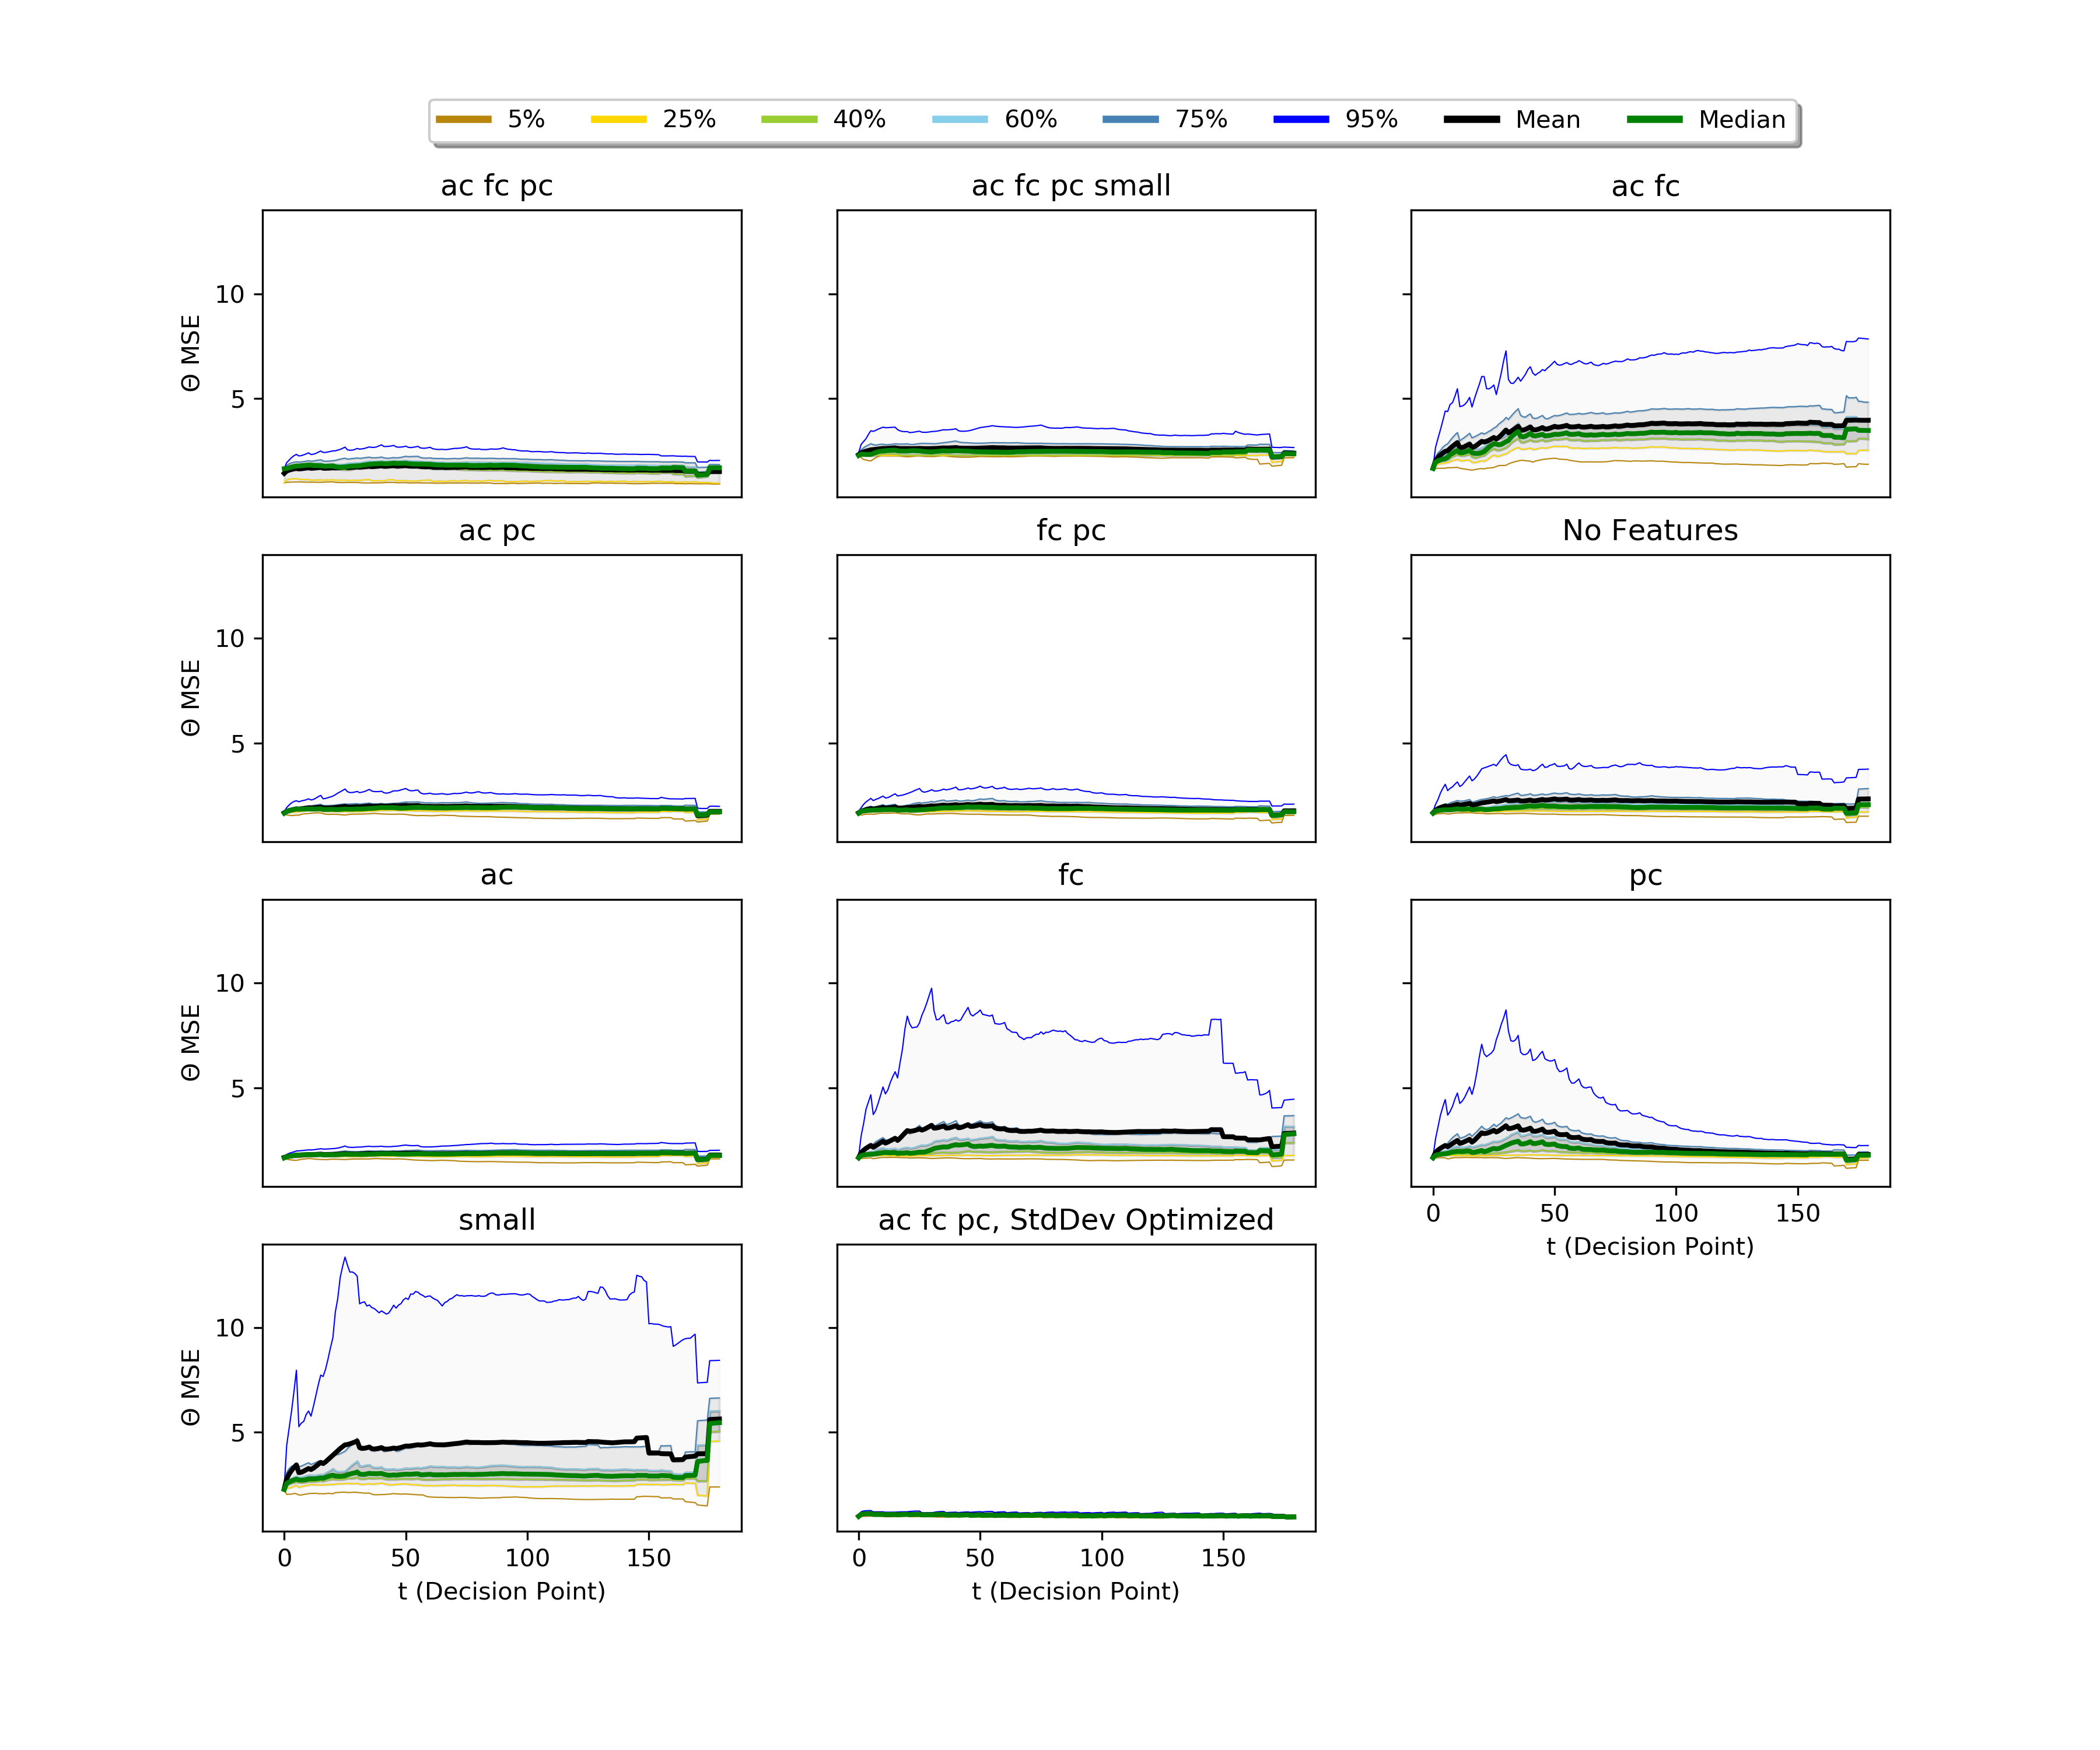
\includegraphics[width=1.5\textwidth,center]{figures/QM11test.png}%
	\caption{Bandit Model $\Theta$ MSE for All Users in Testing Batches}
	\label{QM11test}
	\end{figure}

	\fi



\section{Parameter Tuning vs $MUER$ Figures}

All parameters were tuned in the given range from table \ref{Parameter Optimization Table}, with $160$ steps in between ($160$ chosen to leverage available dedicated \href{https://www.rc.fas.harvard.edu/}{Odyssey Research} cluster computing cores).


\subsection{$MUER$ Minimization Parameter Optimization}
\label{MUER Minimization Parameter Optimization}

	\ifdraft
	Turn off Draft mode to display figures!
	\else
	%%%%%%%%%%%%%%%%%%%%%%%%%%%%%%%%%%%%%%%%%%%%%%%%%%%%%%%%%%%%%%%%%%%%%
	\begin{figure}[H]
	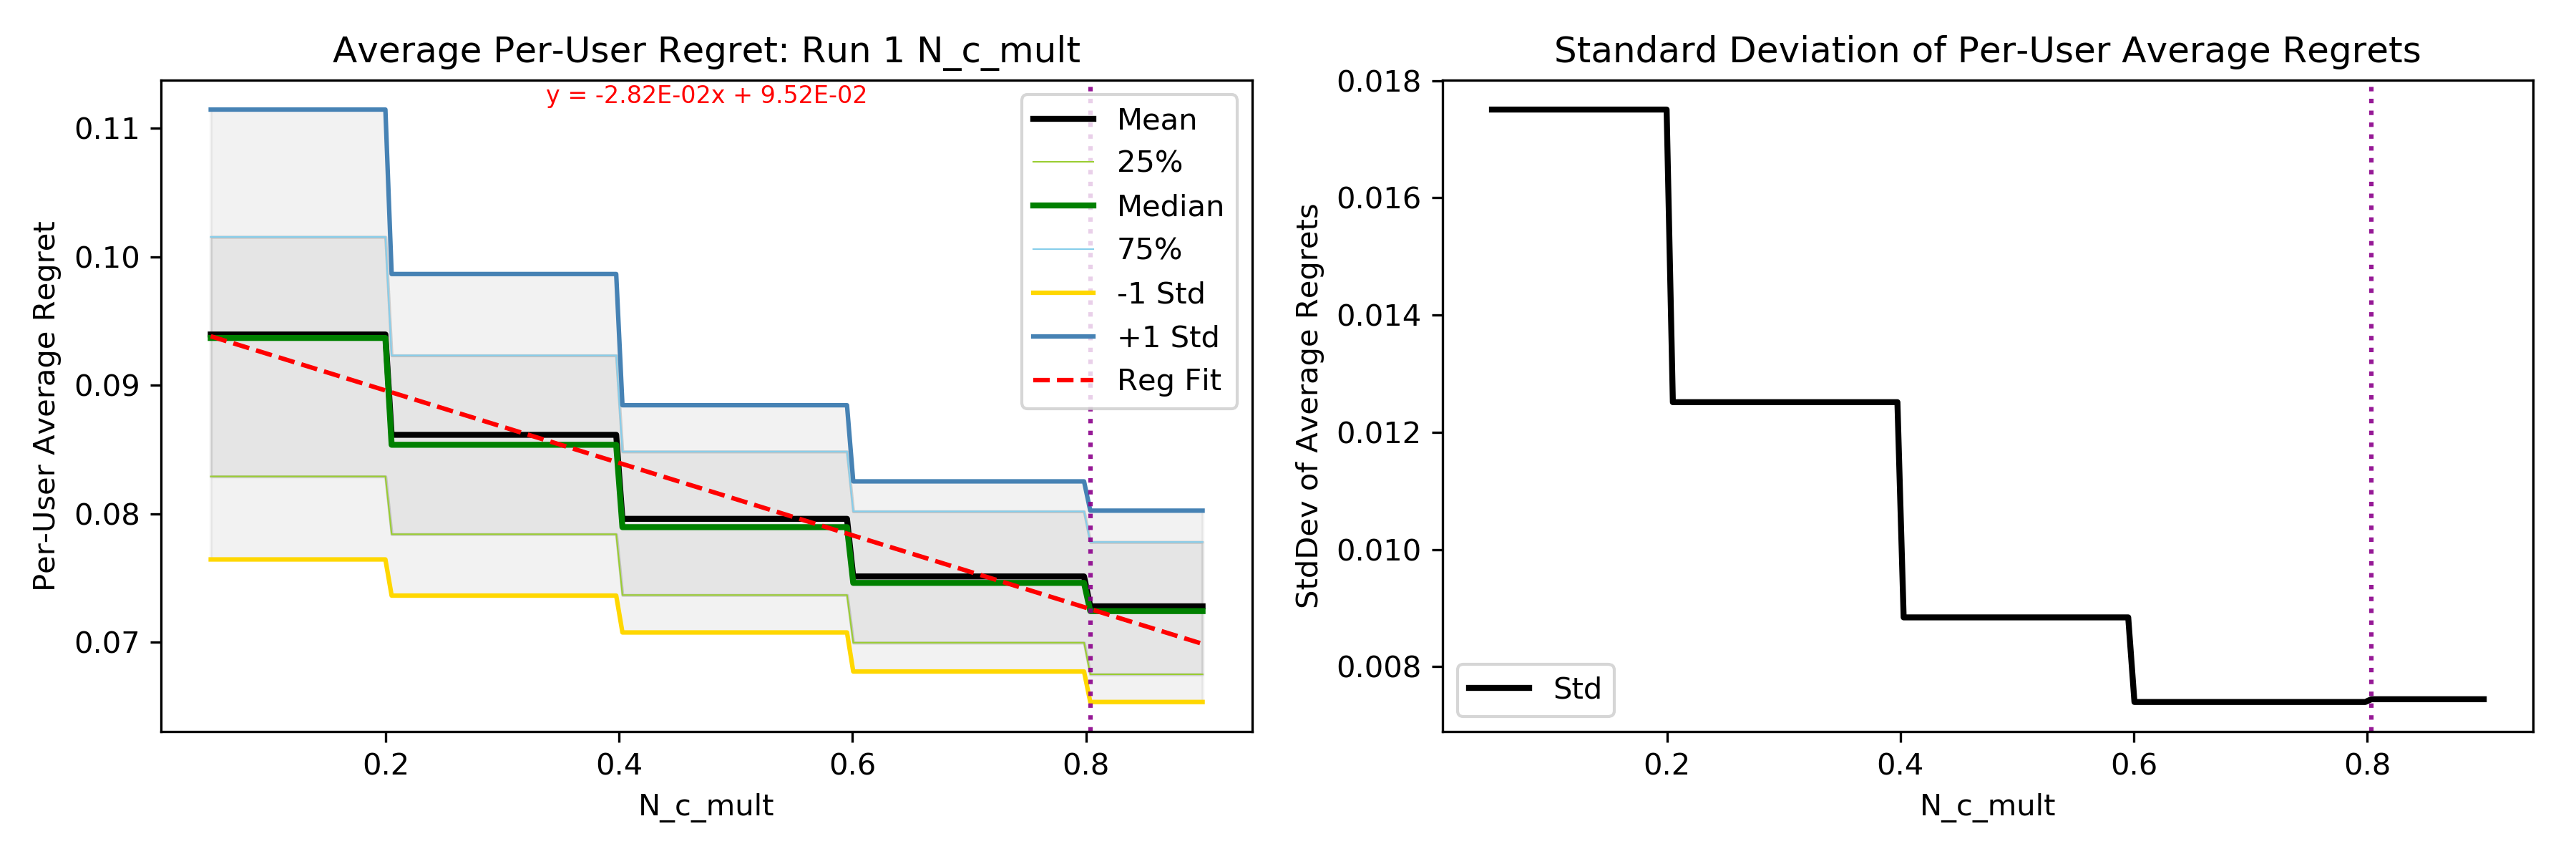
\includegraphics[width=1.1\textwidth,center]{figures/opt_param/opt_param_11100_N_c_mult1.png}%
	\newline
	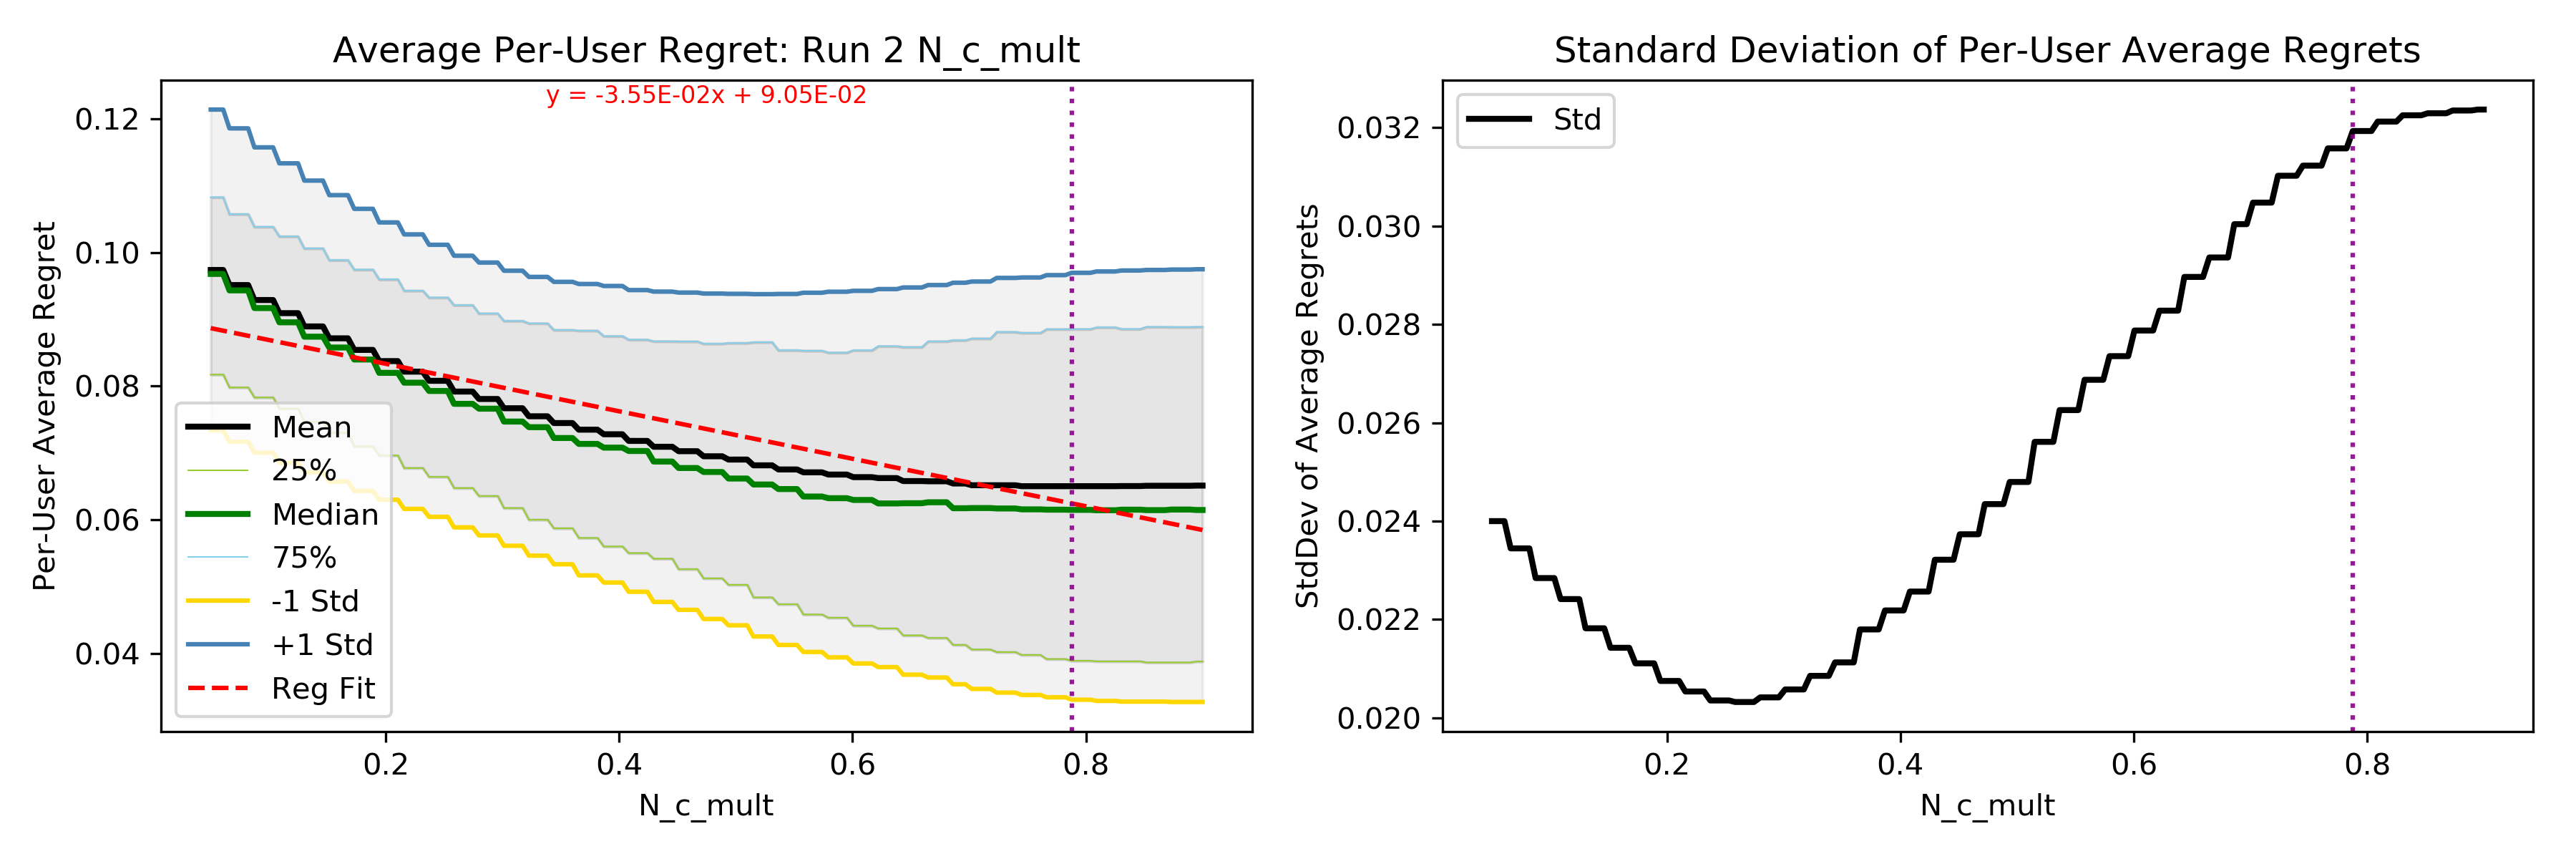
\includegraphics[width=1.1\textwidth,center]{figures/opt_param/opt_param_11100_N_c_mult2.png}%
	\newline
	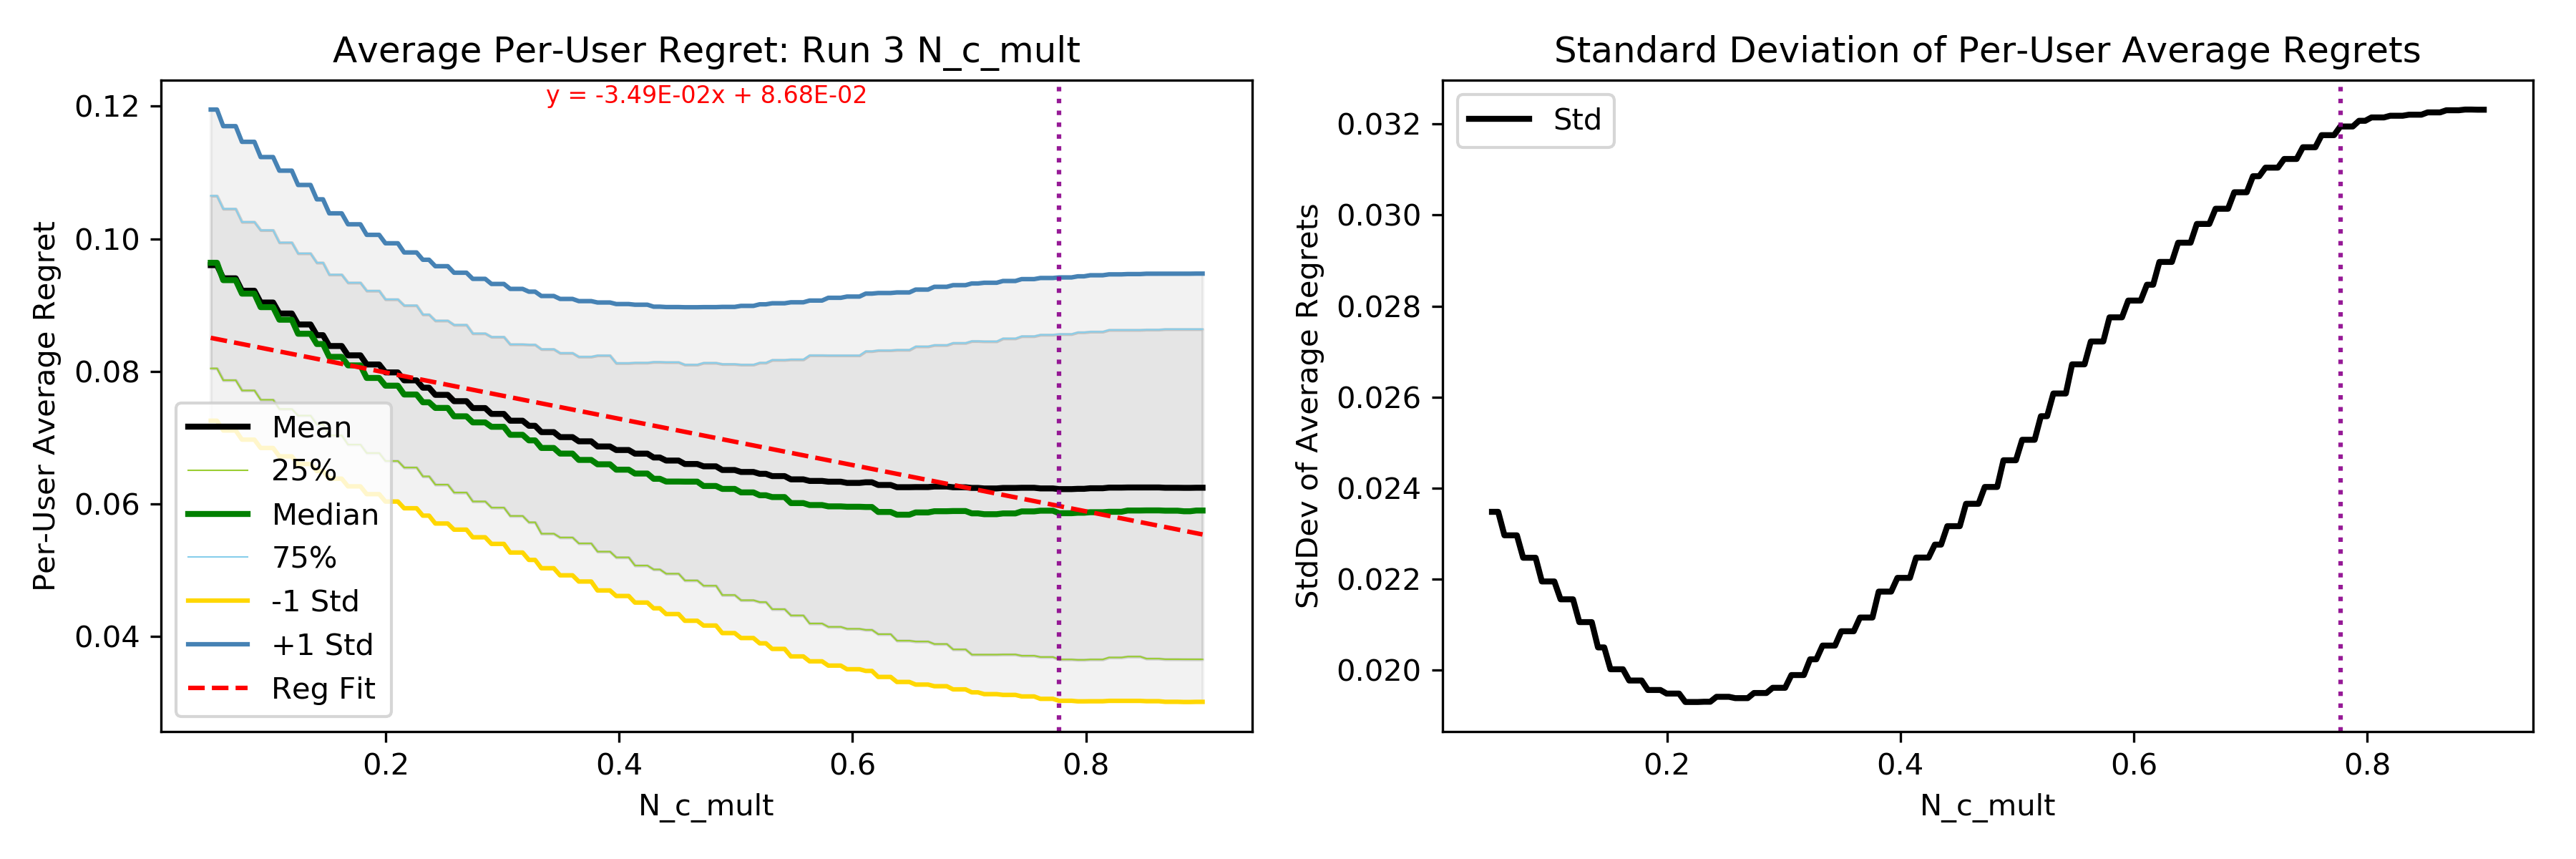
\includegraphics[width=1.1\textwidth,center]{figures/opt_param/opt_param_11100_N_c_mult3.png}%
	\newline
	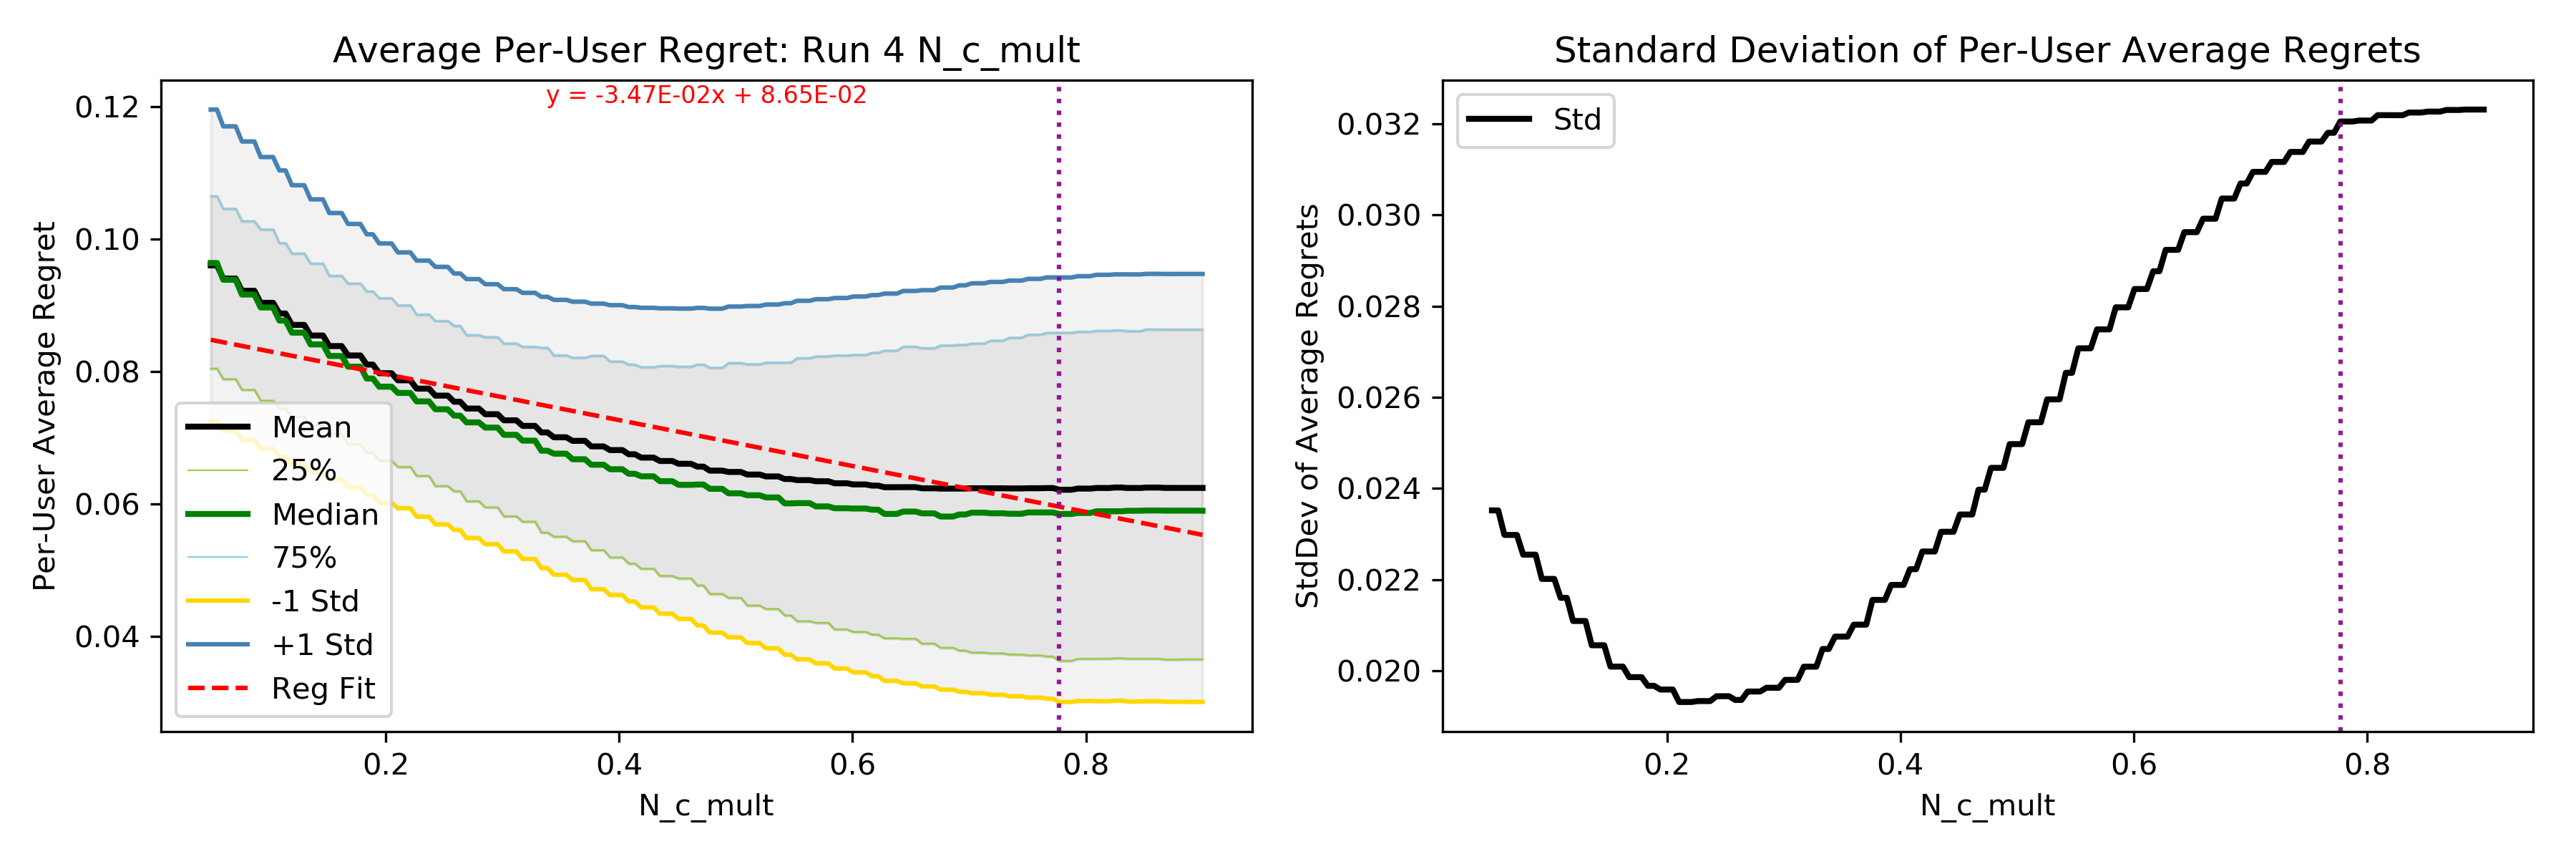
\includegraphics[width=1.1\textwidth,center]{figures/opt_param/opt_param_11100_N_c_mult4.png}%
	\caption{$MUER$ for Varying $\mathtt{N\_c\_mult}$, $MUER$ Minimization Optimization}
	\end{figure}

	\begin{figure}[H]
	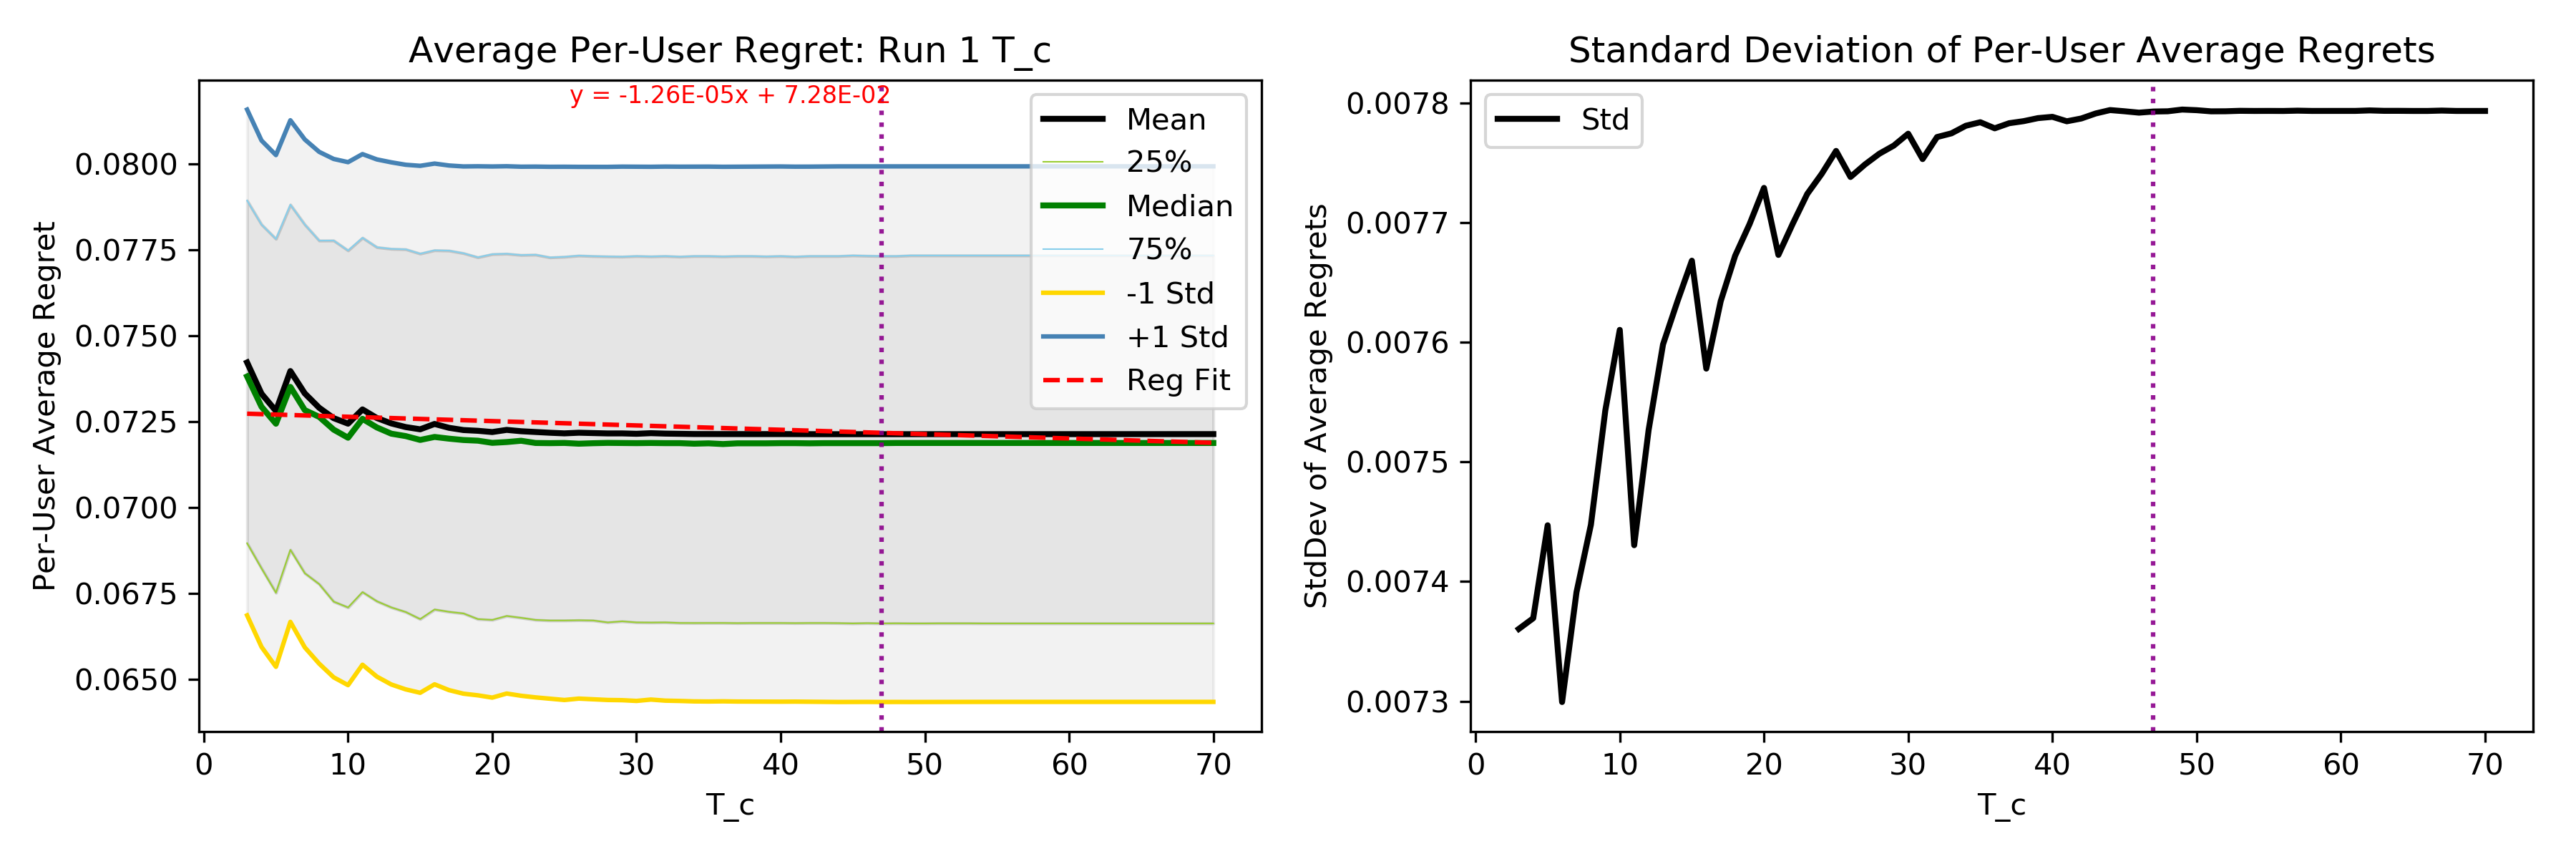
\includegraphics[width=1.1\textwidth,center]{figures/opt_param/opt_param_11100_T_c1.png}%
	\newline
	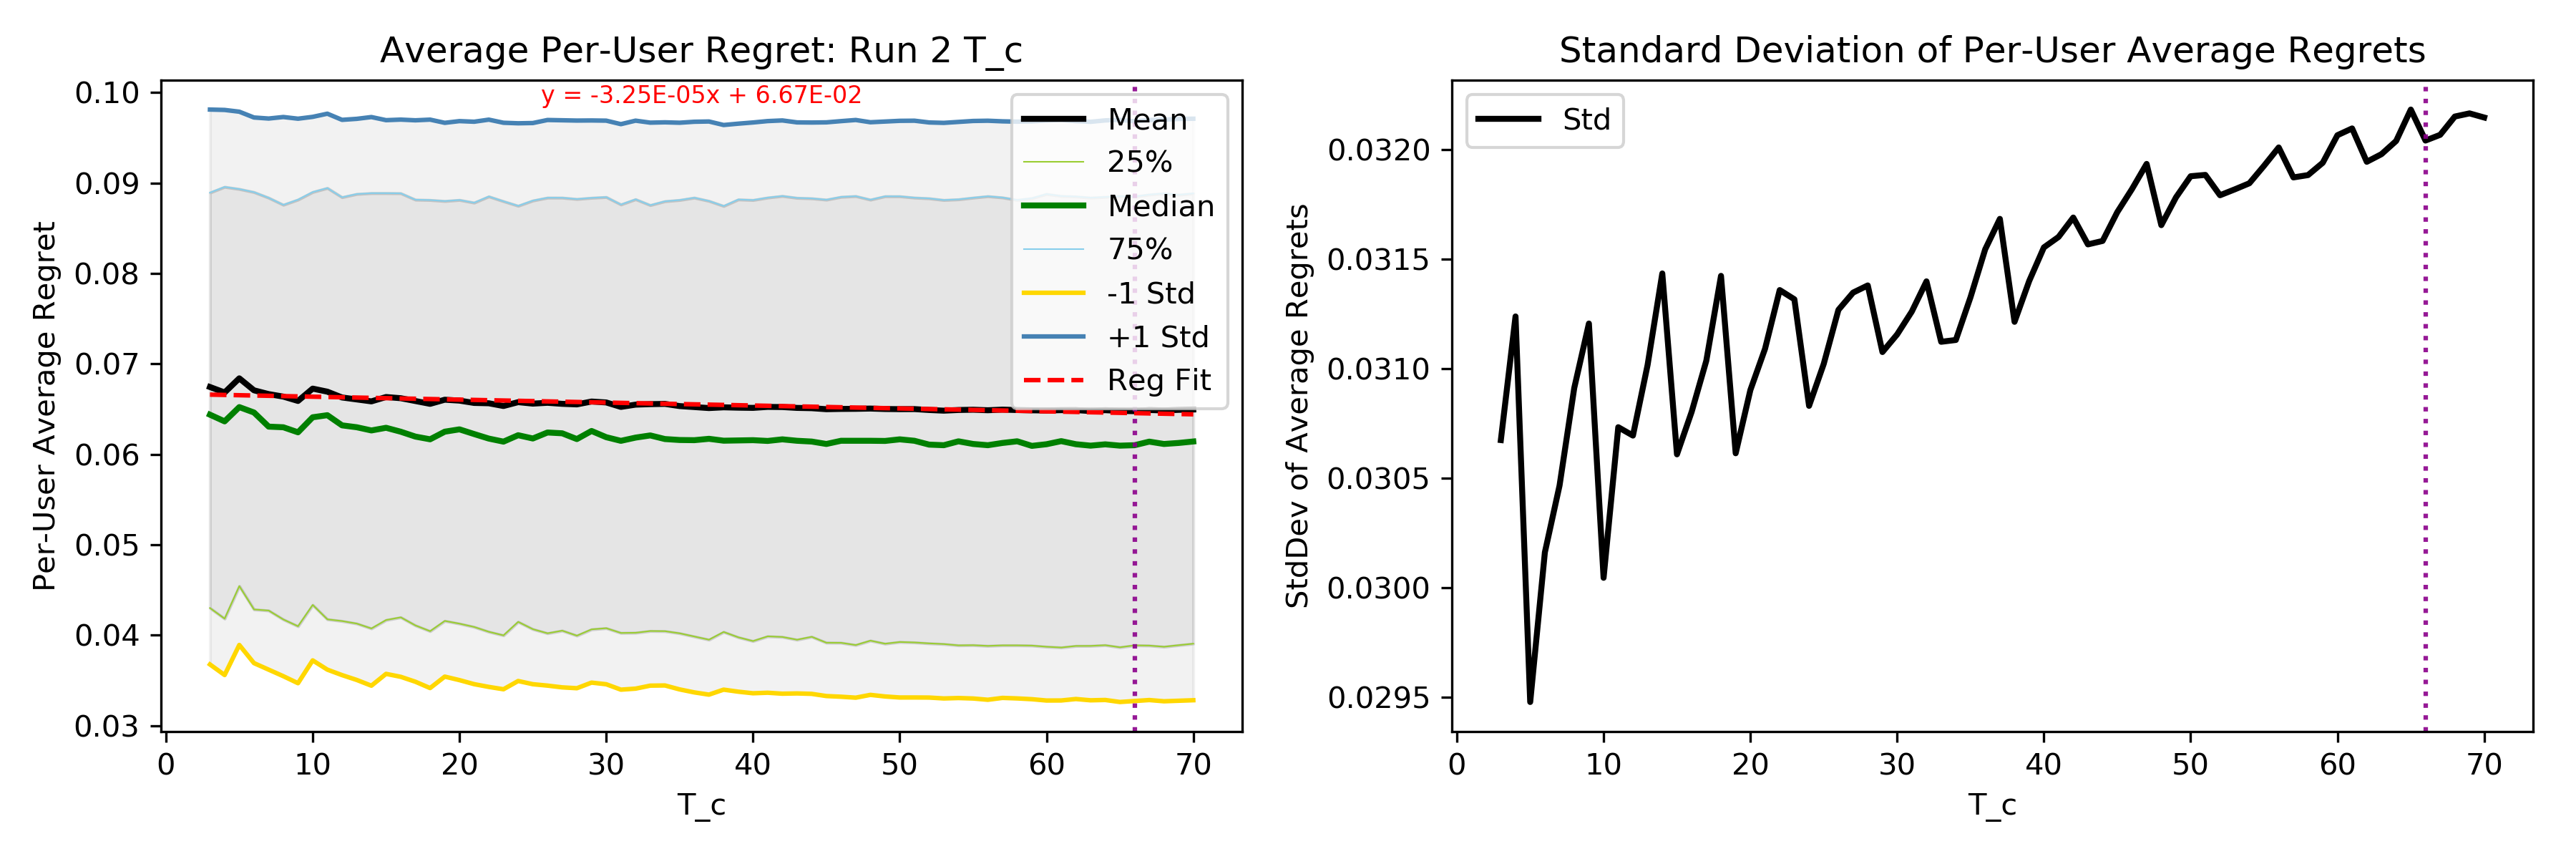
\includegraphics[width=1.1\textwidth,center]{figures/opt_param/opt_param_11100_T_c2.png}%
	\newline
	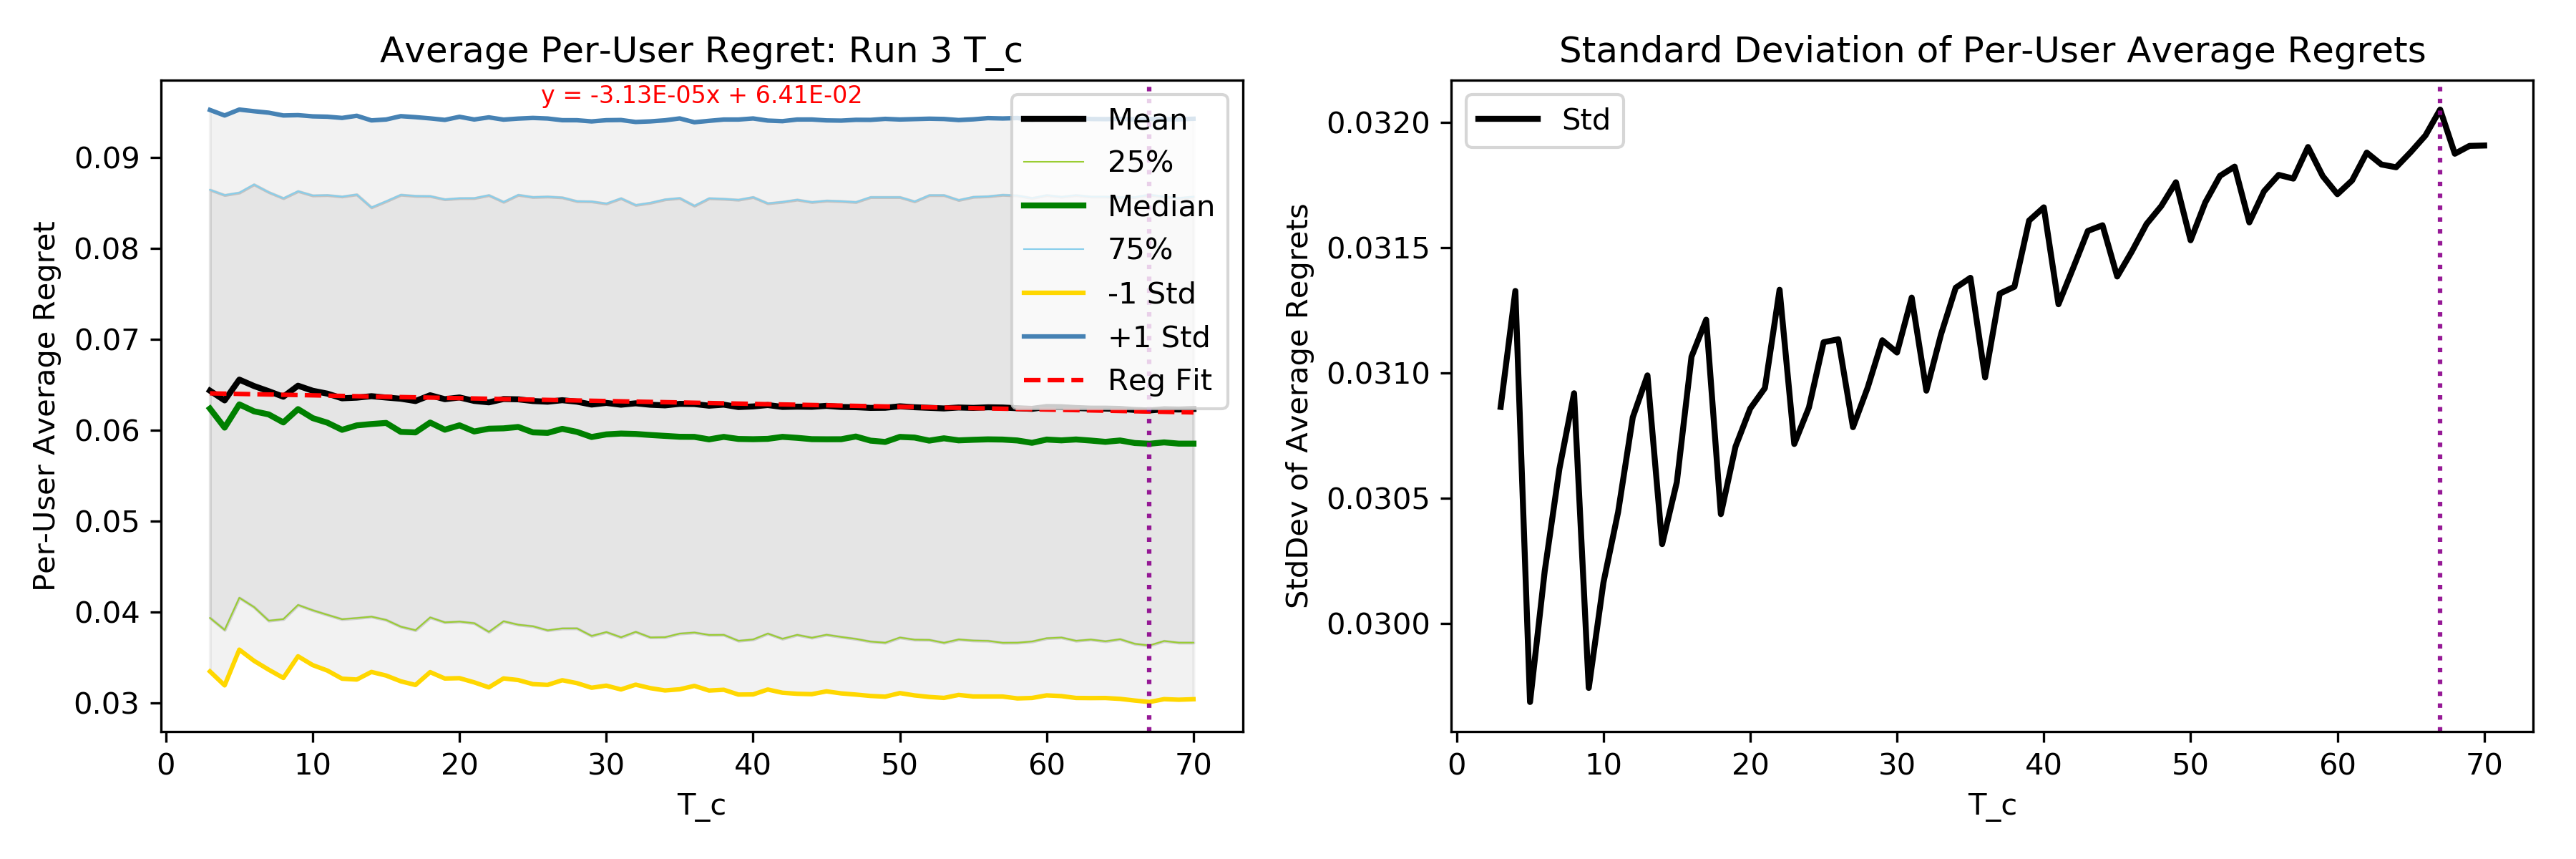
\includegraphics[width=1.1\textwidth,center]{figures/opt_param/opt_param_11100_T_c3.png}%
	\newline
	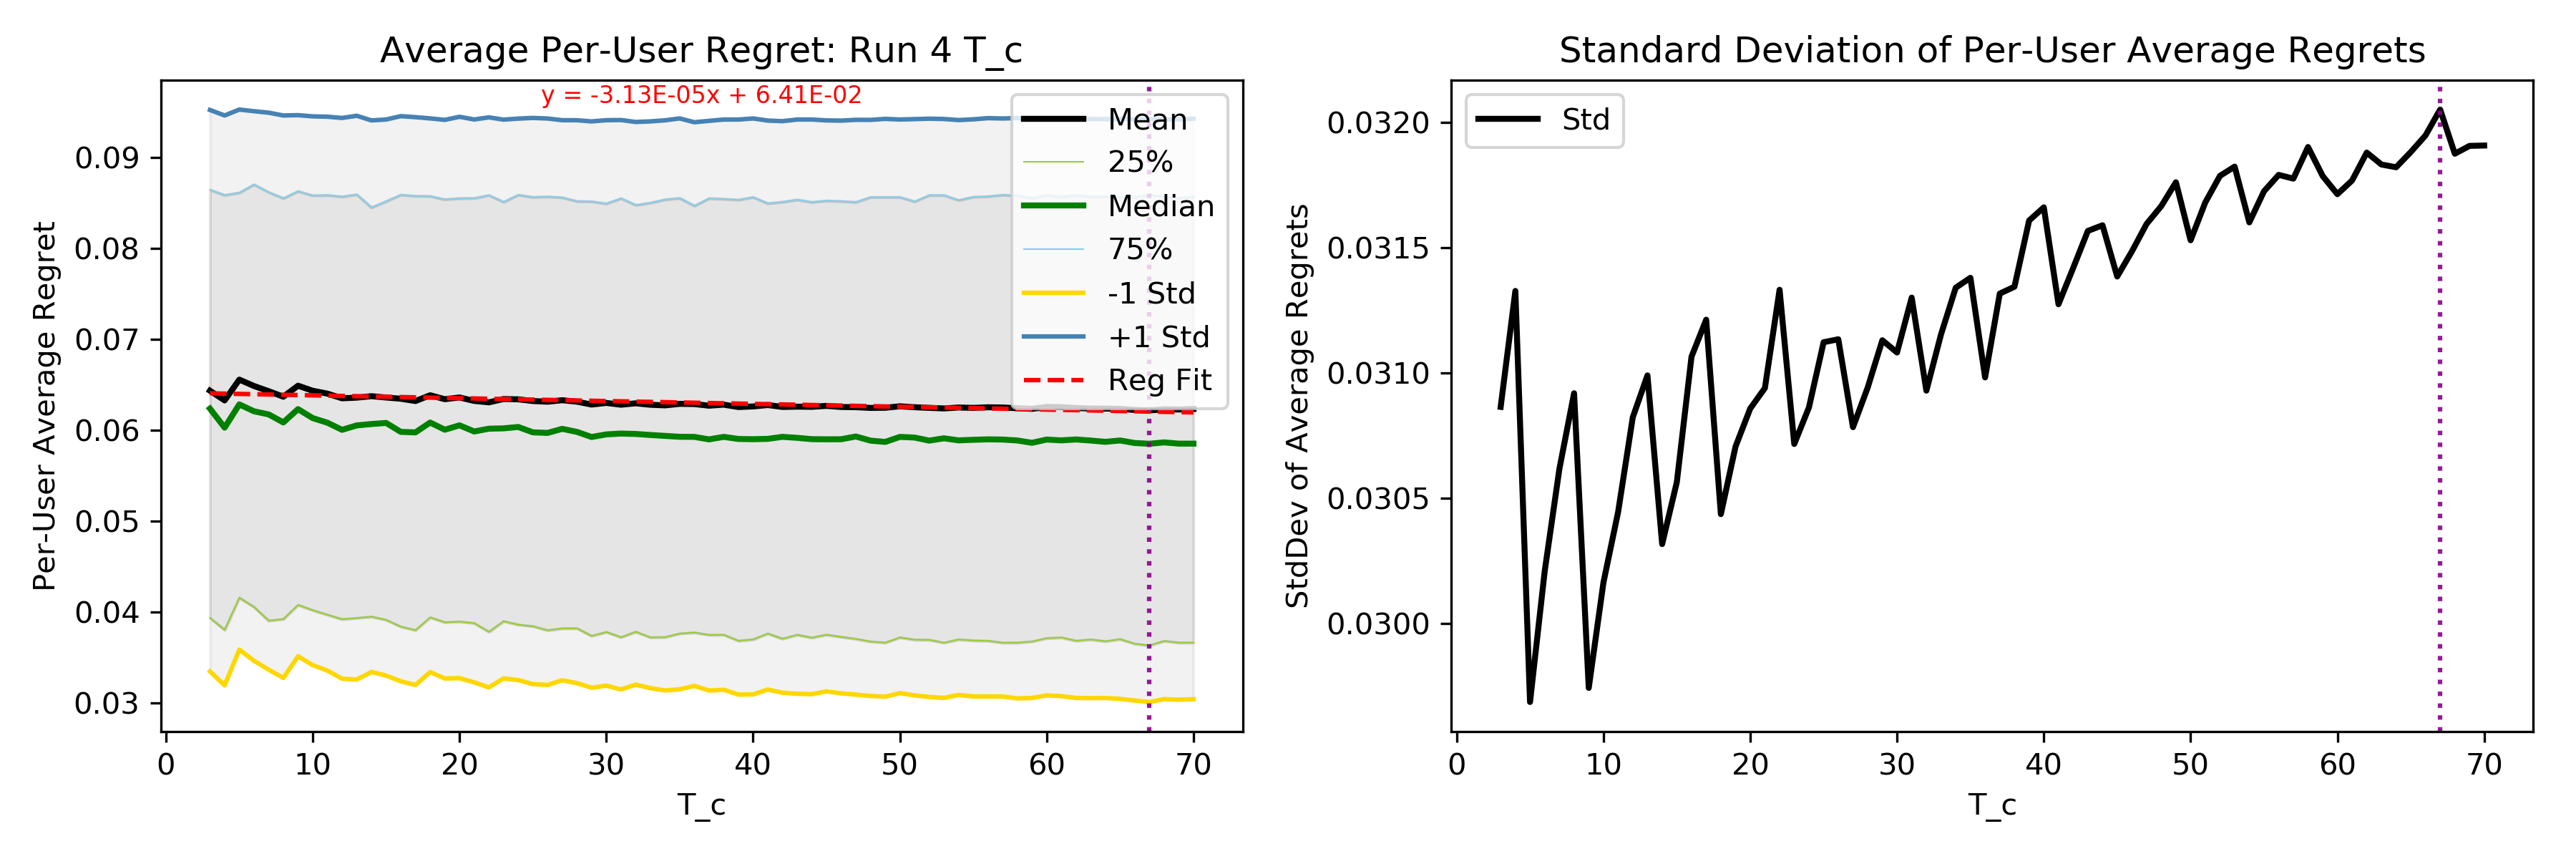
\includegraphics[width=1.1\textwidth,center]{figures/opt_param/opt_param_11100_T_c4.png}%
	\caption{$MUER$ for Varying $\mathtt{T\_c}$, $MUER$ Minimization Optimization}
	\end{figure}

	\begin{figure}[H]
	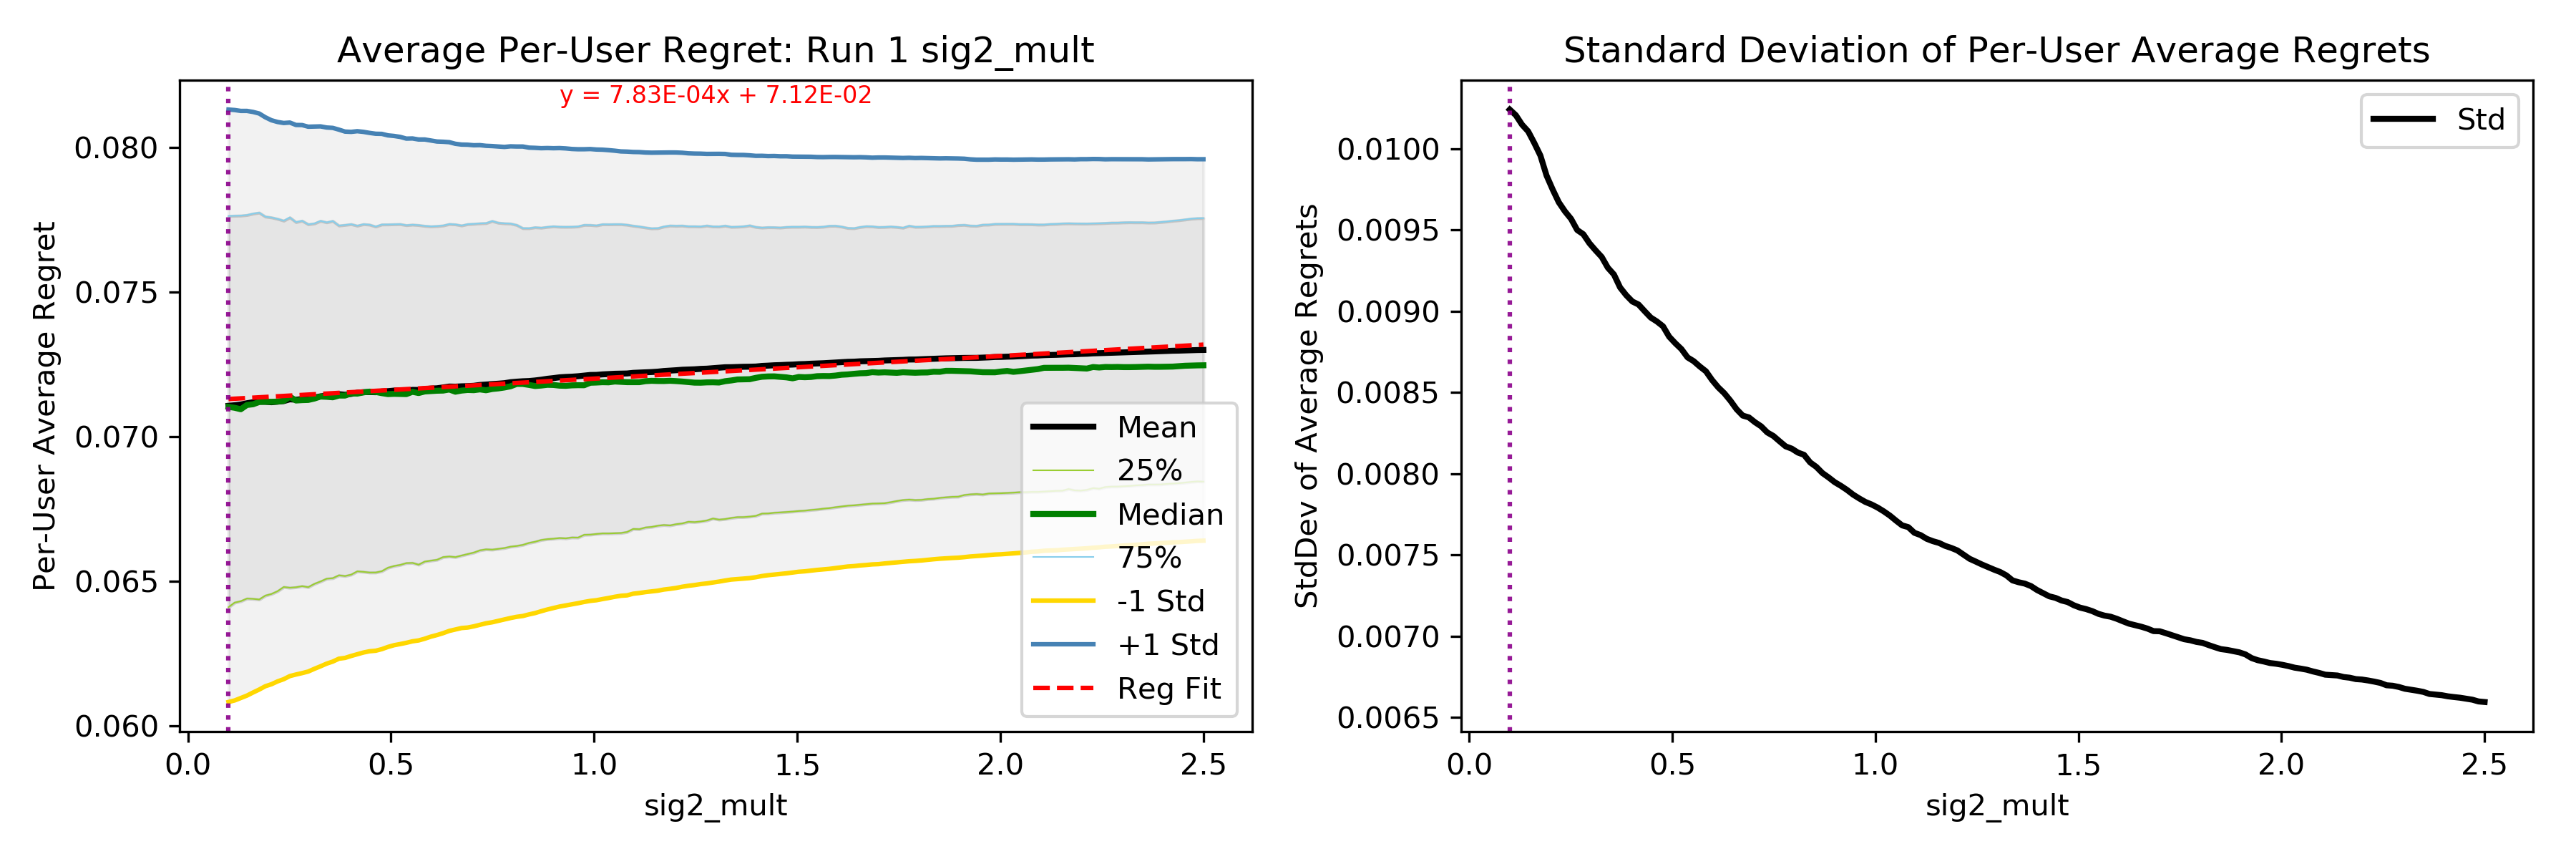
\includegraphics[width=1.1\textwidth,center]{figures/opt_param/opt_param_11100_sig2_mult1.png}%
	\newline
	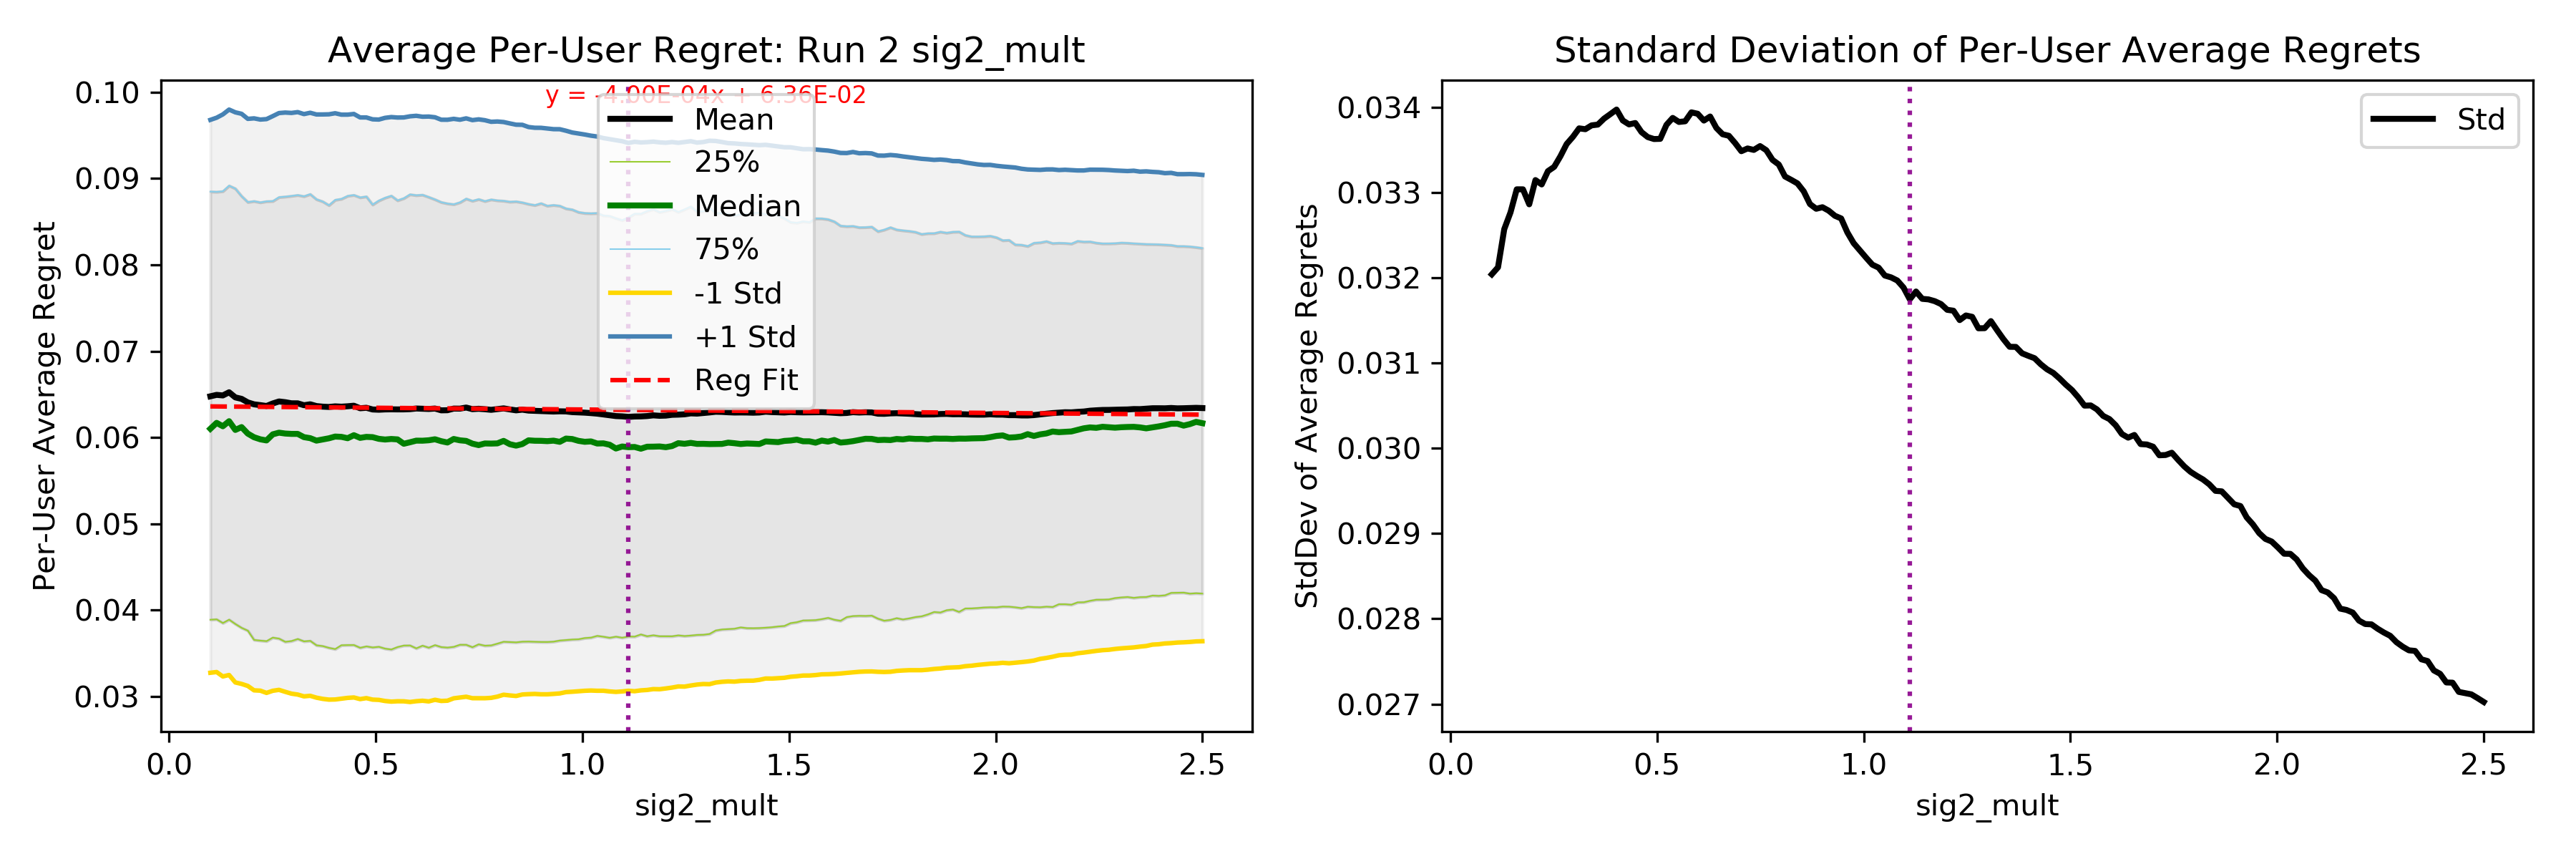
\includegraphics[width=1.1\textwidth,center]{figures/opt_param/opt_param_11100_sig2_mult2.png}%
	\newline
	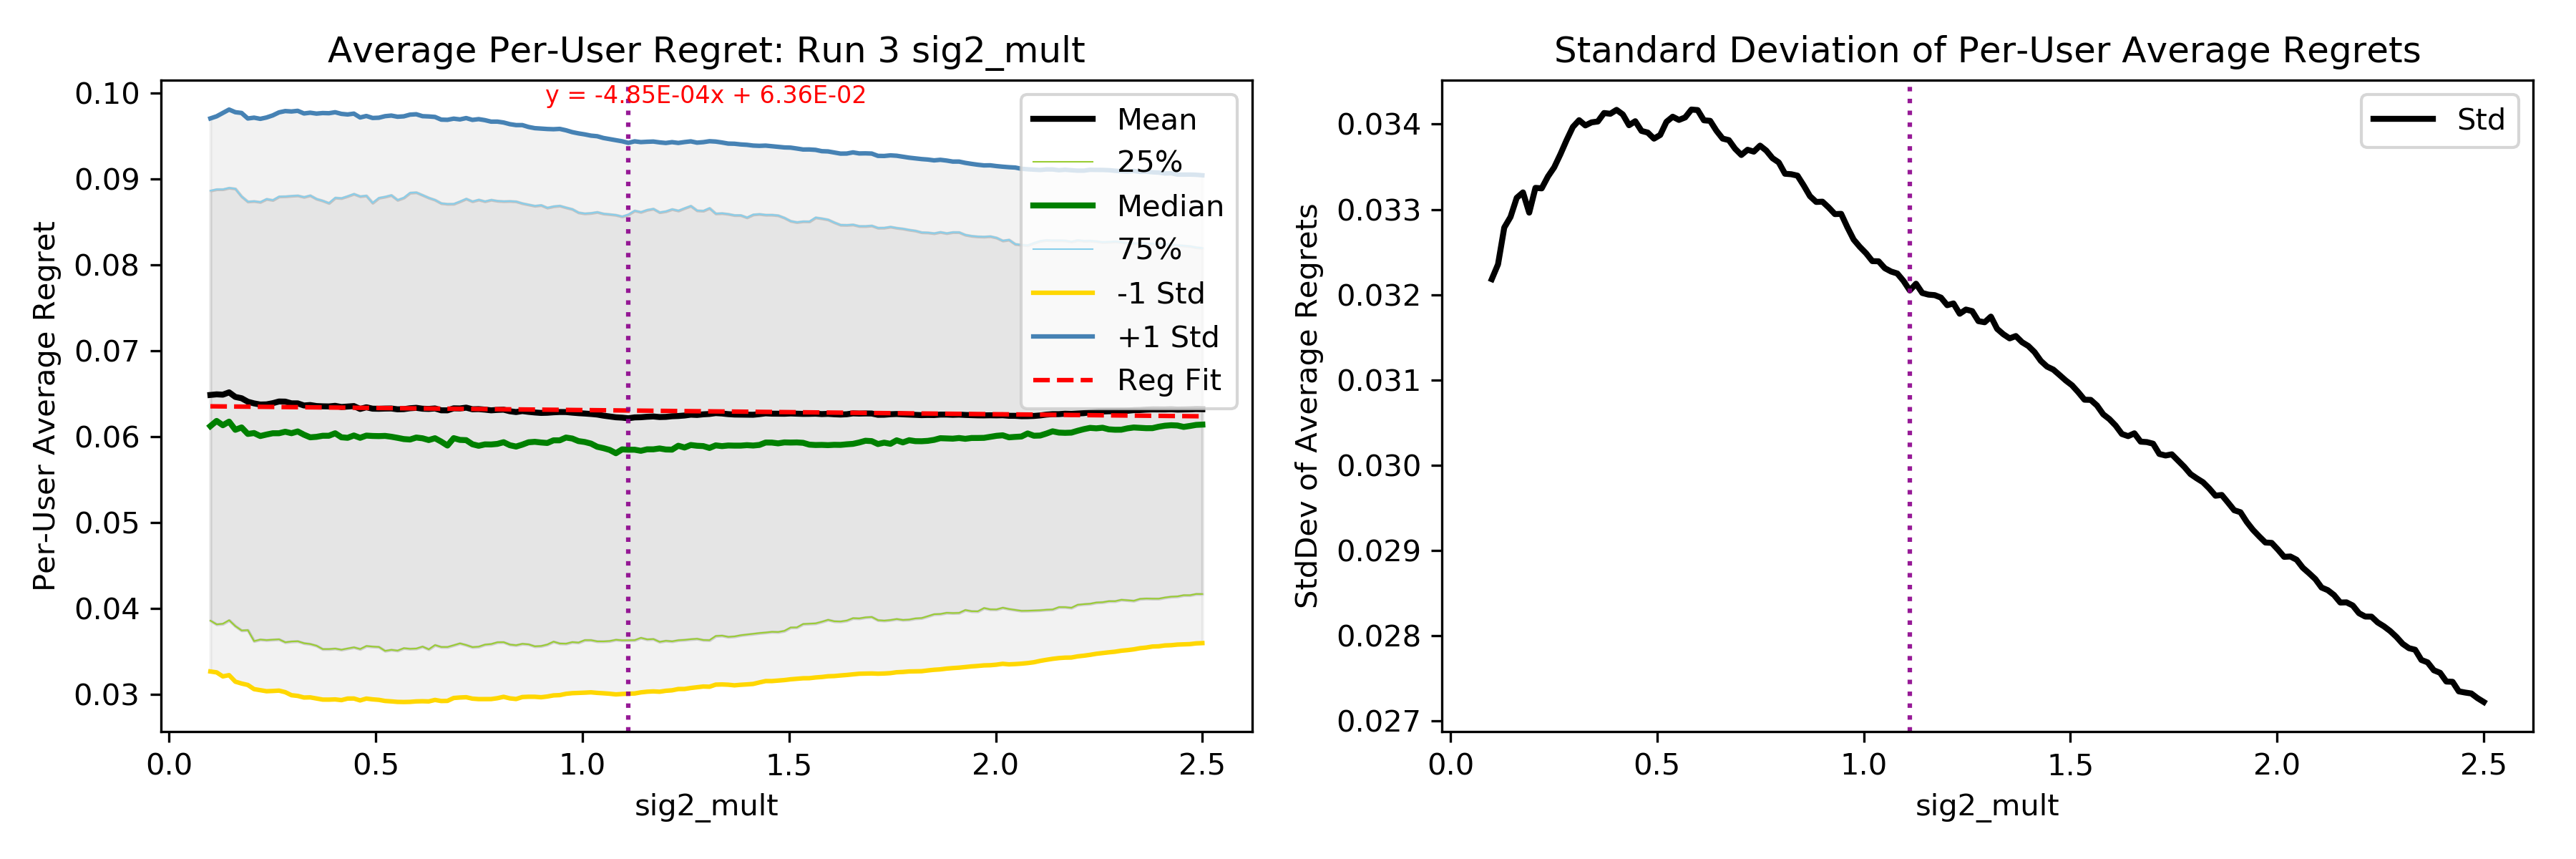
\includegraphics[width=1.1\textwidth,center]{figures/opt_param/opt_param_11100_sig2_mult3.png}%
	\newline
	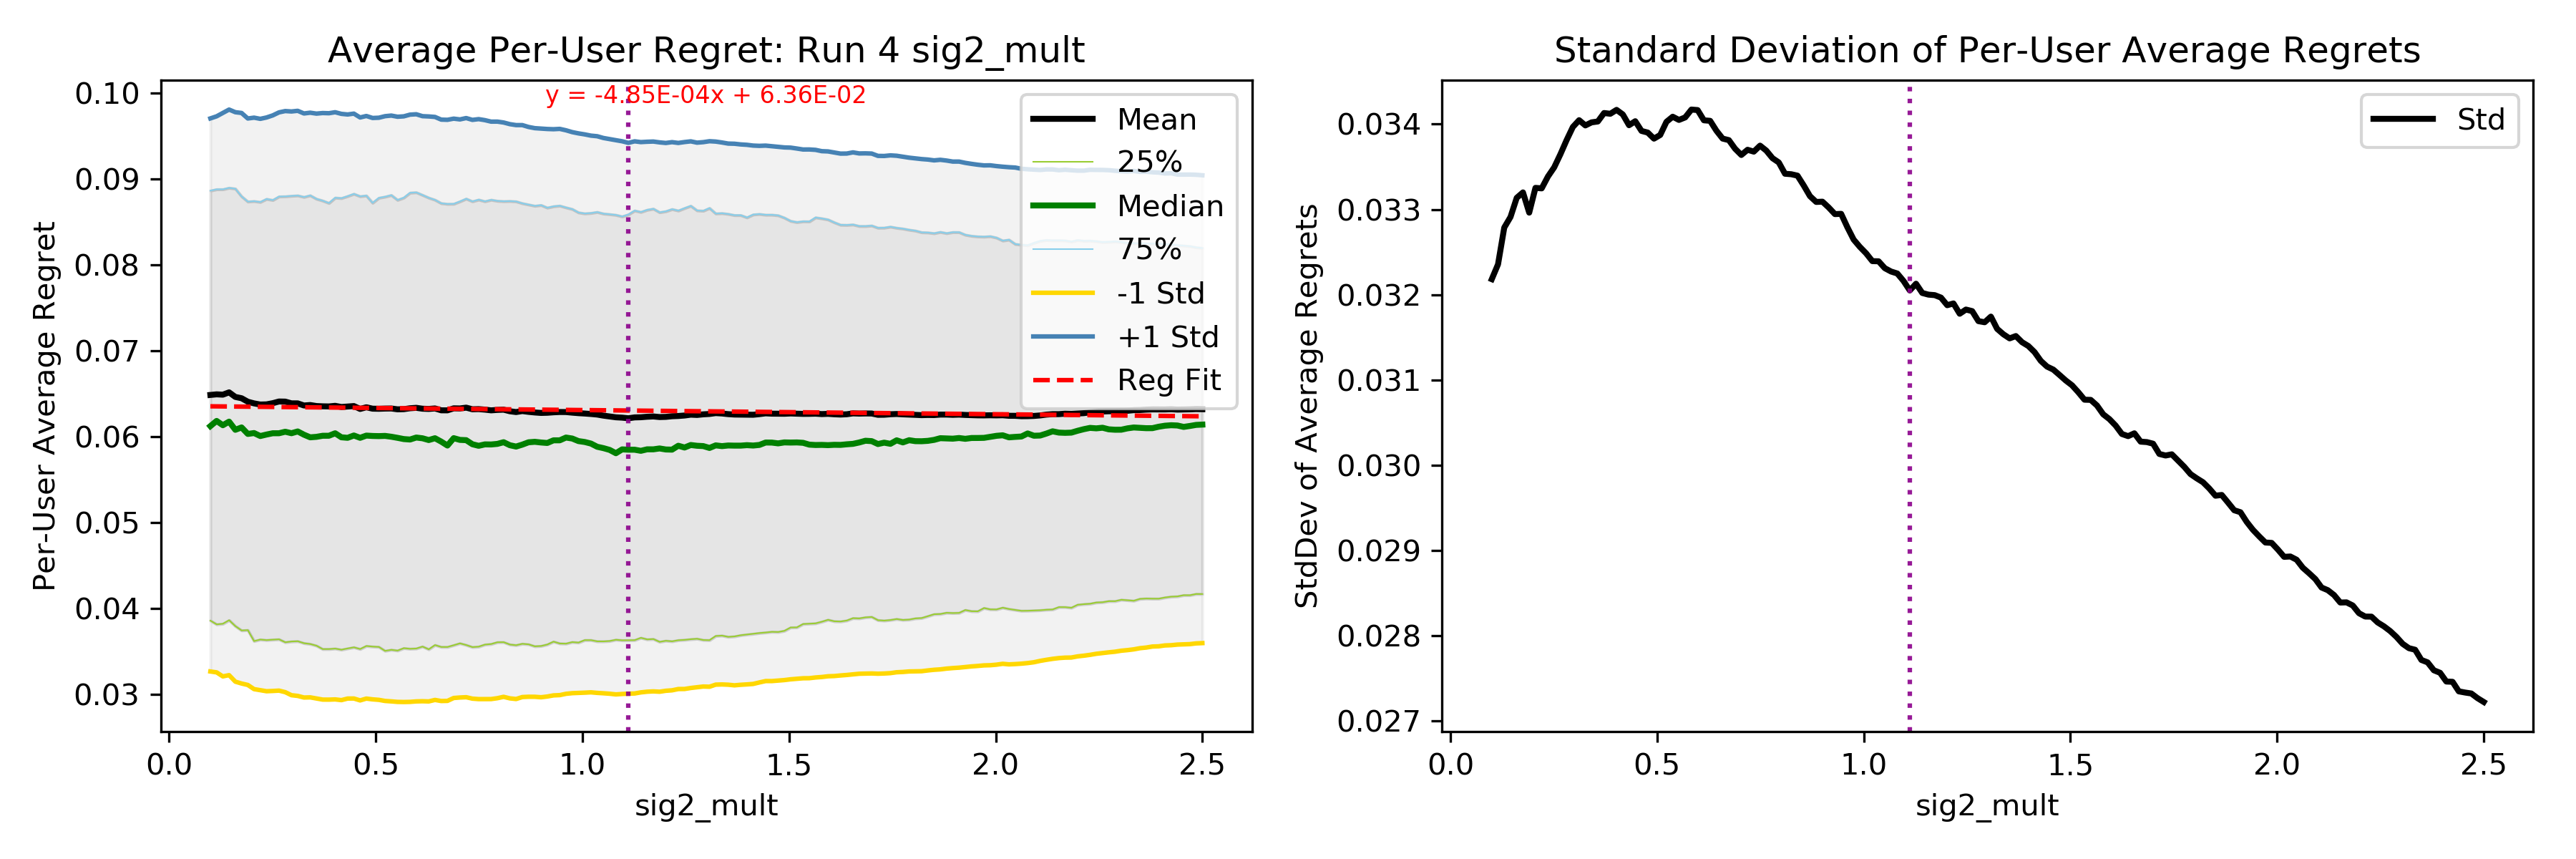
\includegraphics[width=1.1\textwidth,center]{figures/opt_param/opt_param_11100_sig2_mult4.png}%
	\caption{$MUER$ for Varying $\mathtt{sig2\_mult}$, $MUER$ Minimization Optimization}
	\end{figure}

	\begin{figure}[H]
	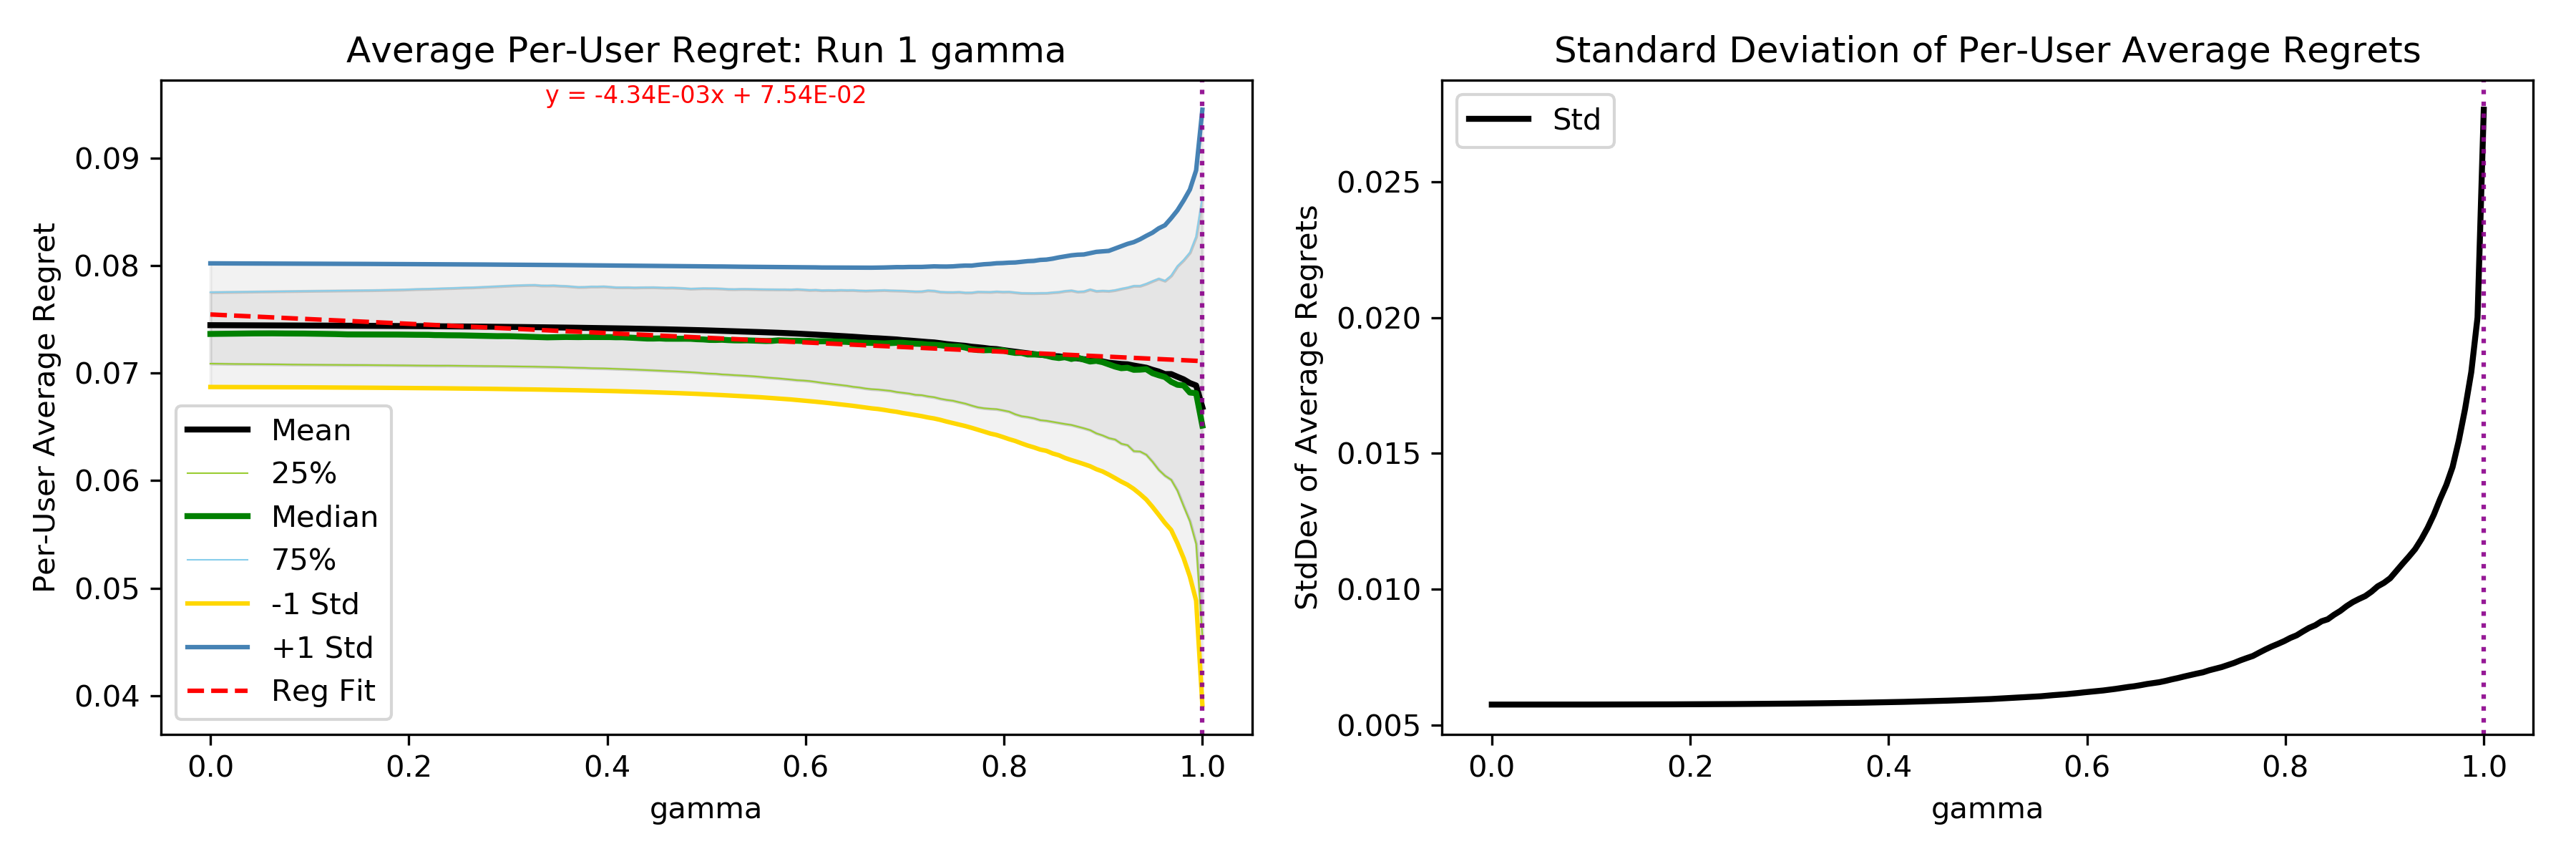
\includegraphics[width=1.1\textwidth,center]{figures/opt_param/opt_param_11100_gamma1.png}%
	\newline
	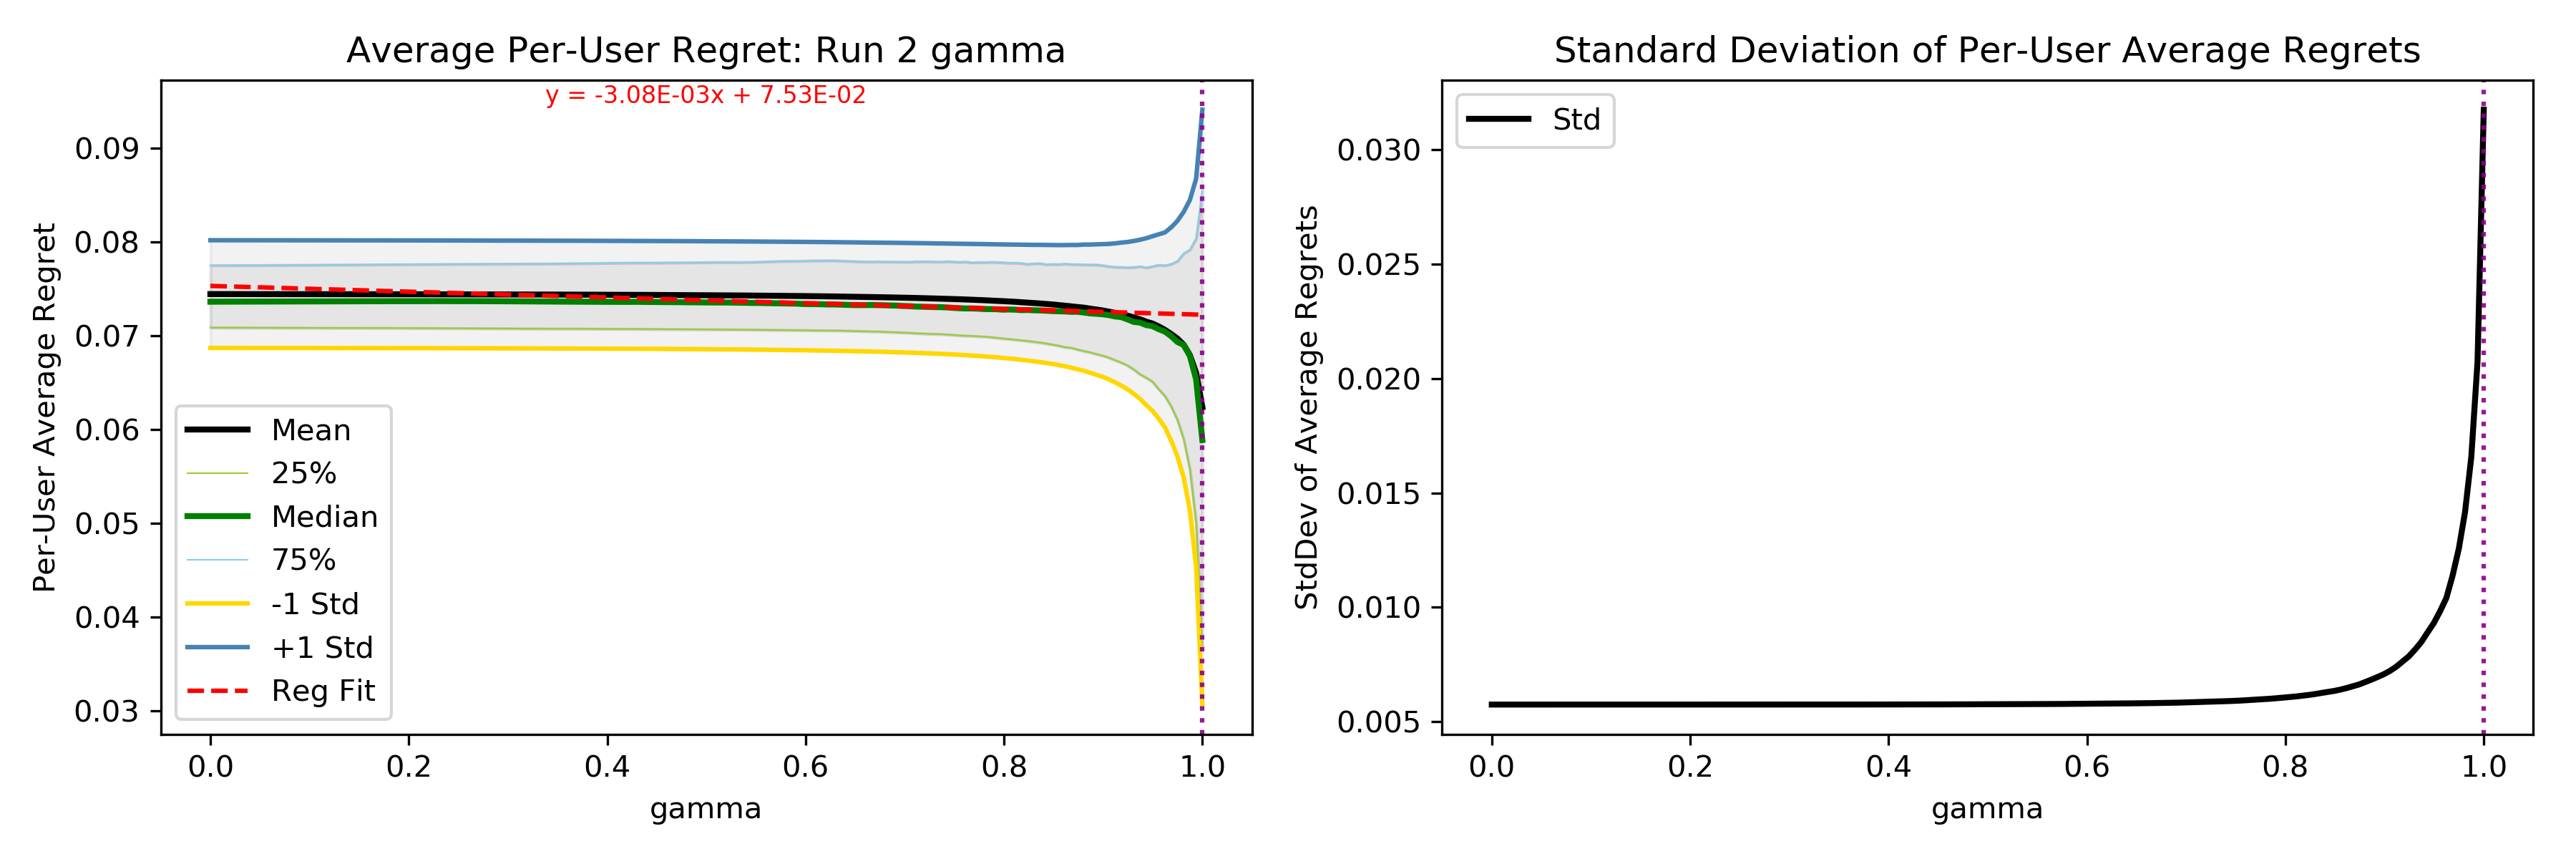
\includegraphics[width=1.1\textwidth,center]{figures/opt_param/opt_param_11100_gamma2.png}%
	\newline
	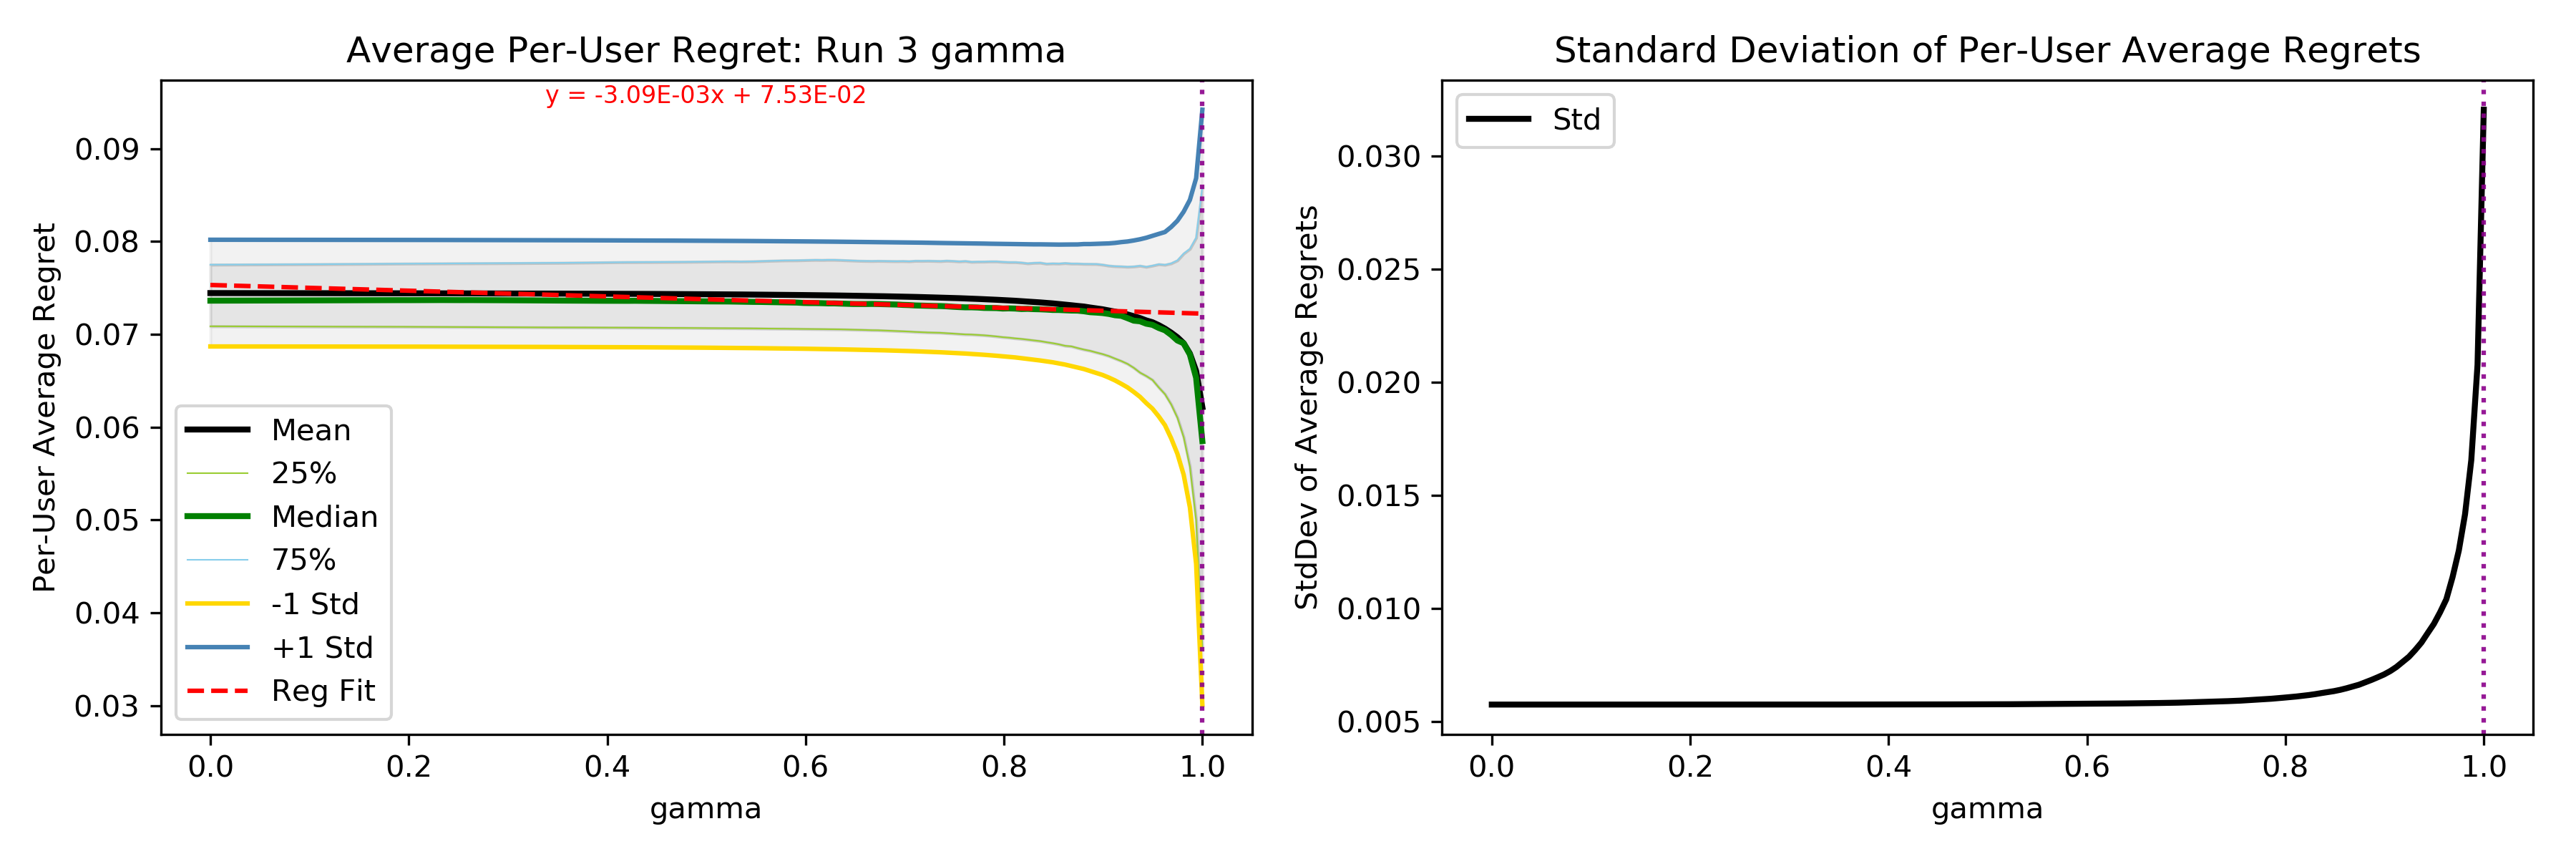
\includegraphics[width=1.1\textwidth,center]{figures/opt_param/opt_param_11100_gamma3.png}%
	\newline
	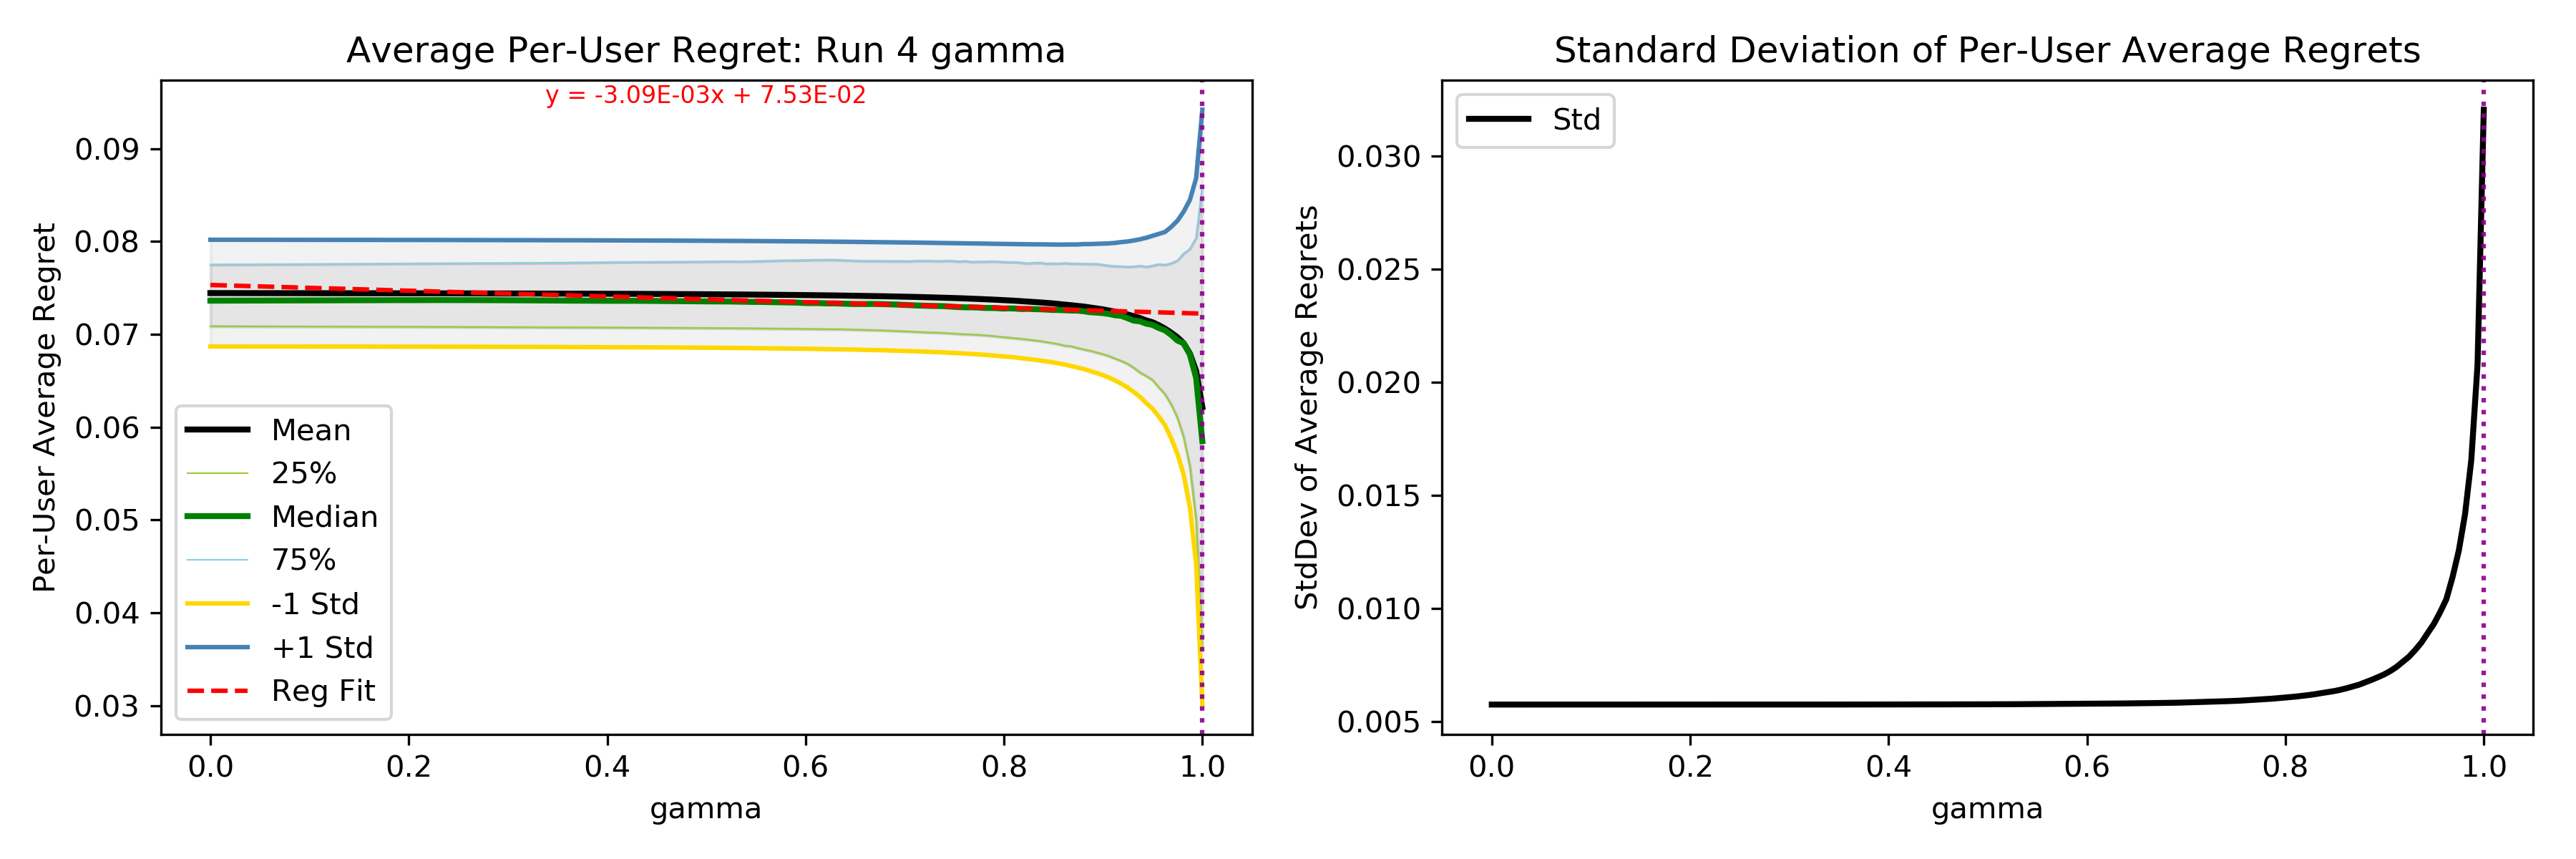
\includegraphics[width=1.1\textwidth,center]{figures/opt_param/opt_param_11100_gamma4.png}%
	\caption{$MUER$ for Varying $\mathtt{gamma}$, $MUER$ Minimization Optimization}
	\end{figure}

	\begin{figure}[H]
	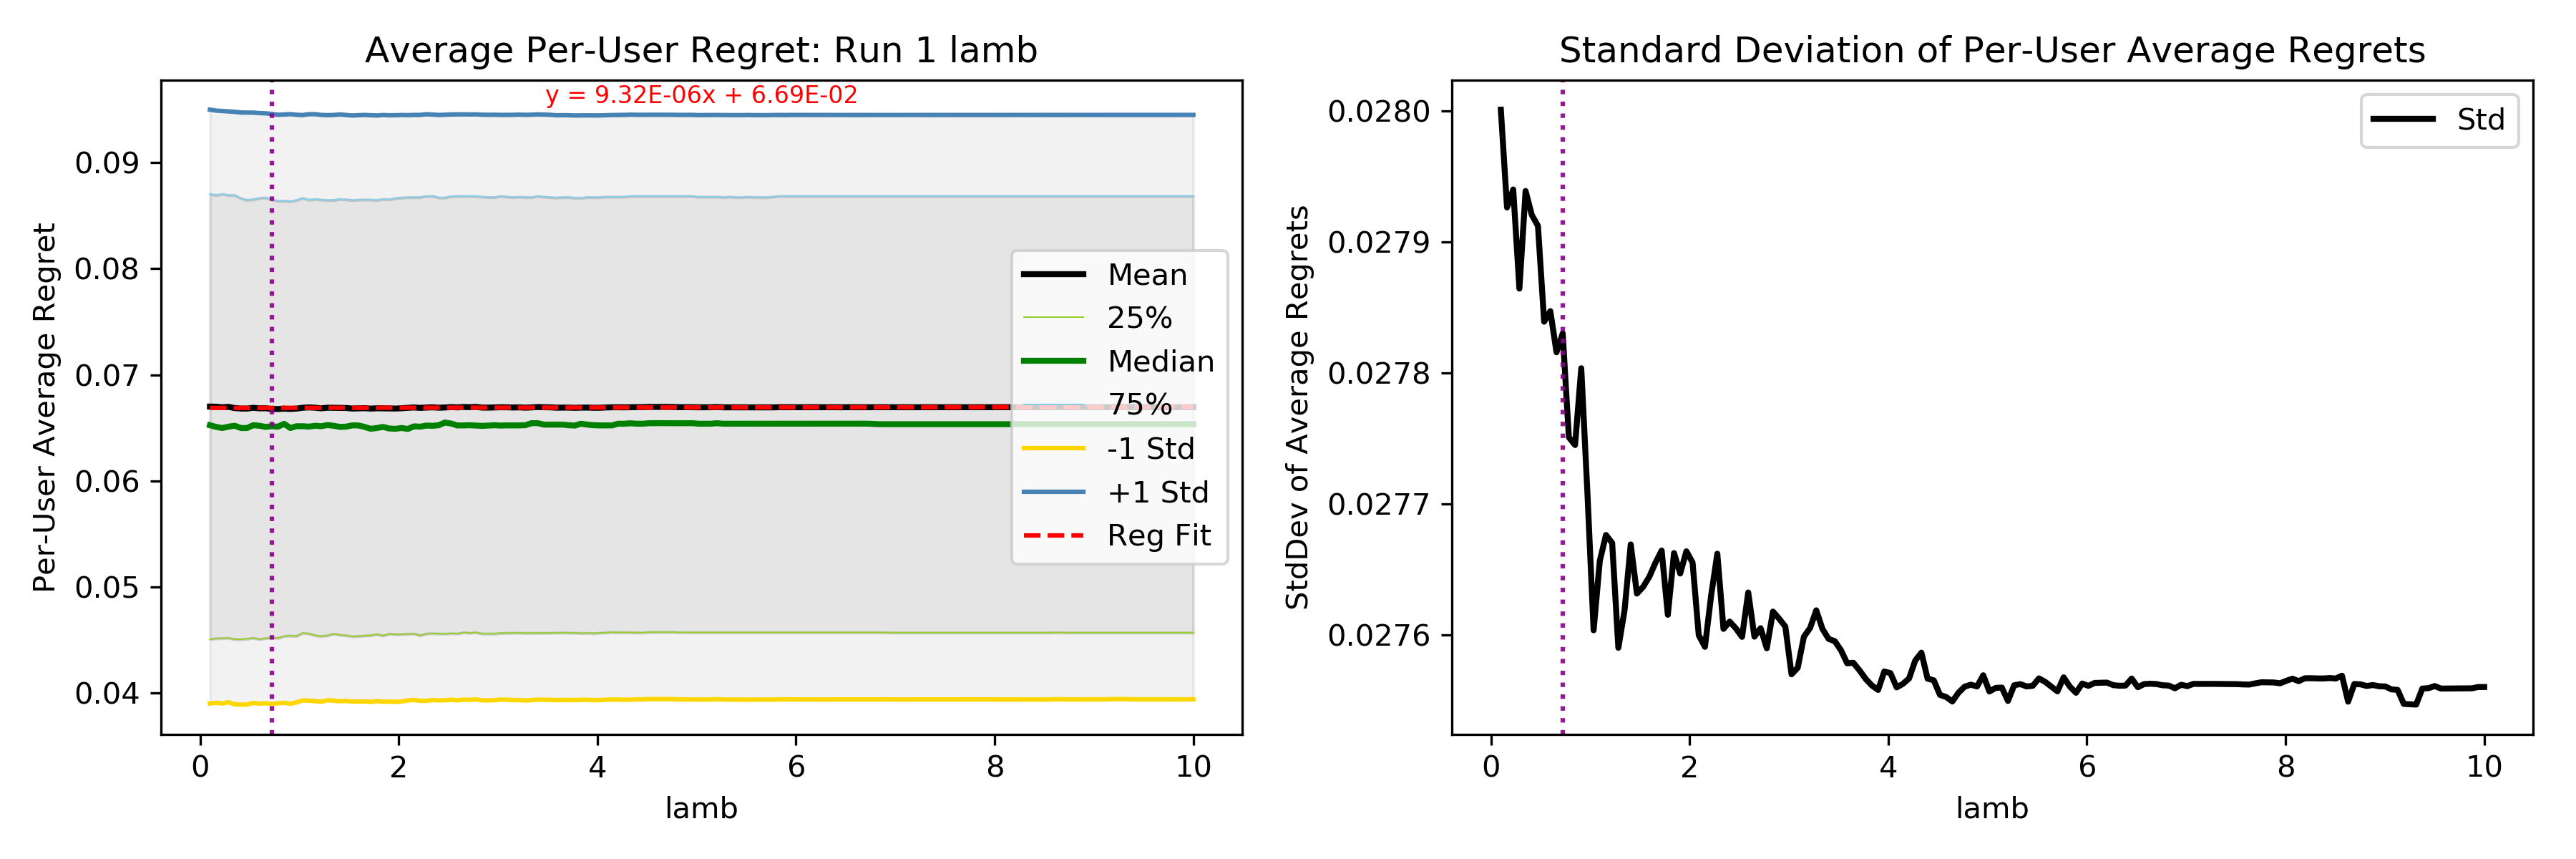
\includegraphics[width=1.1\textwidth,center]{figures/opt_param/opt_param_11100_lamb1.png}%
	\newline
	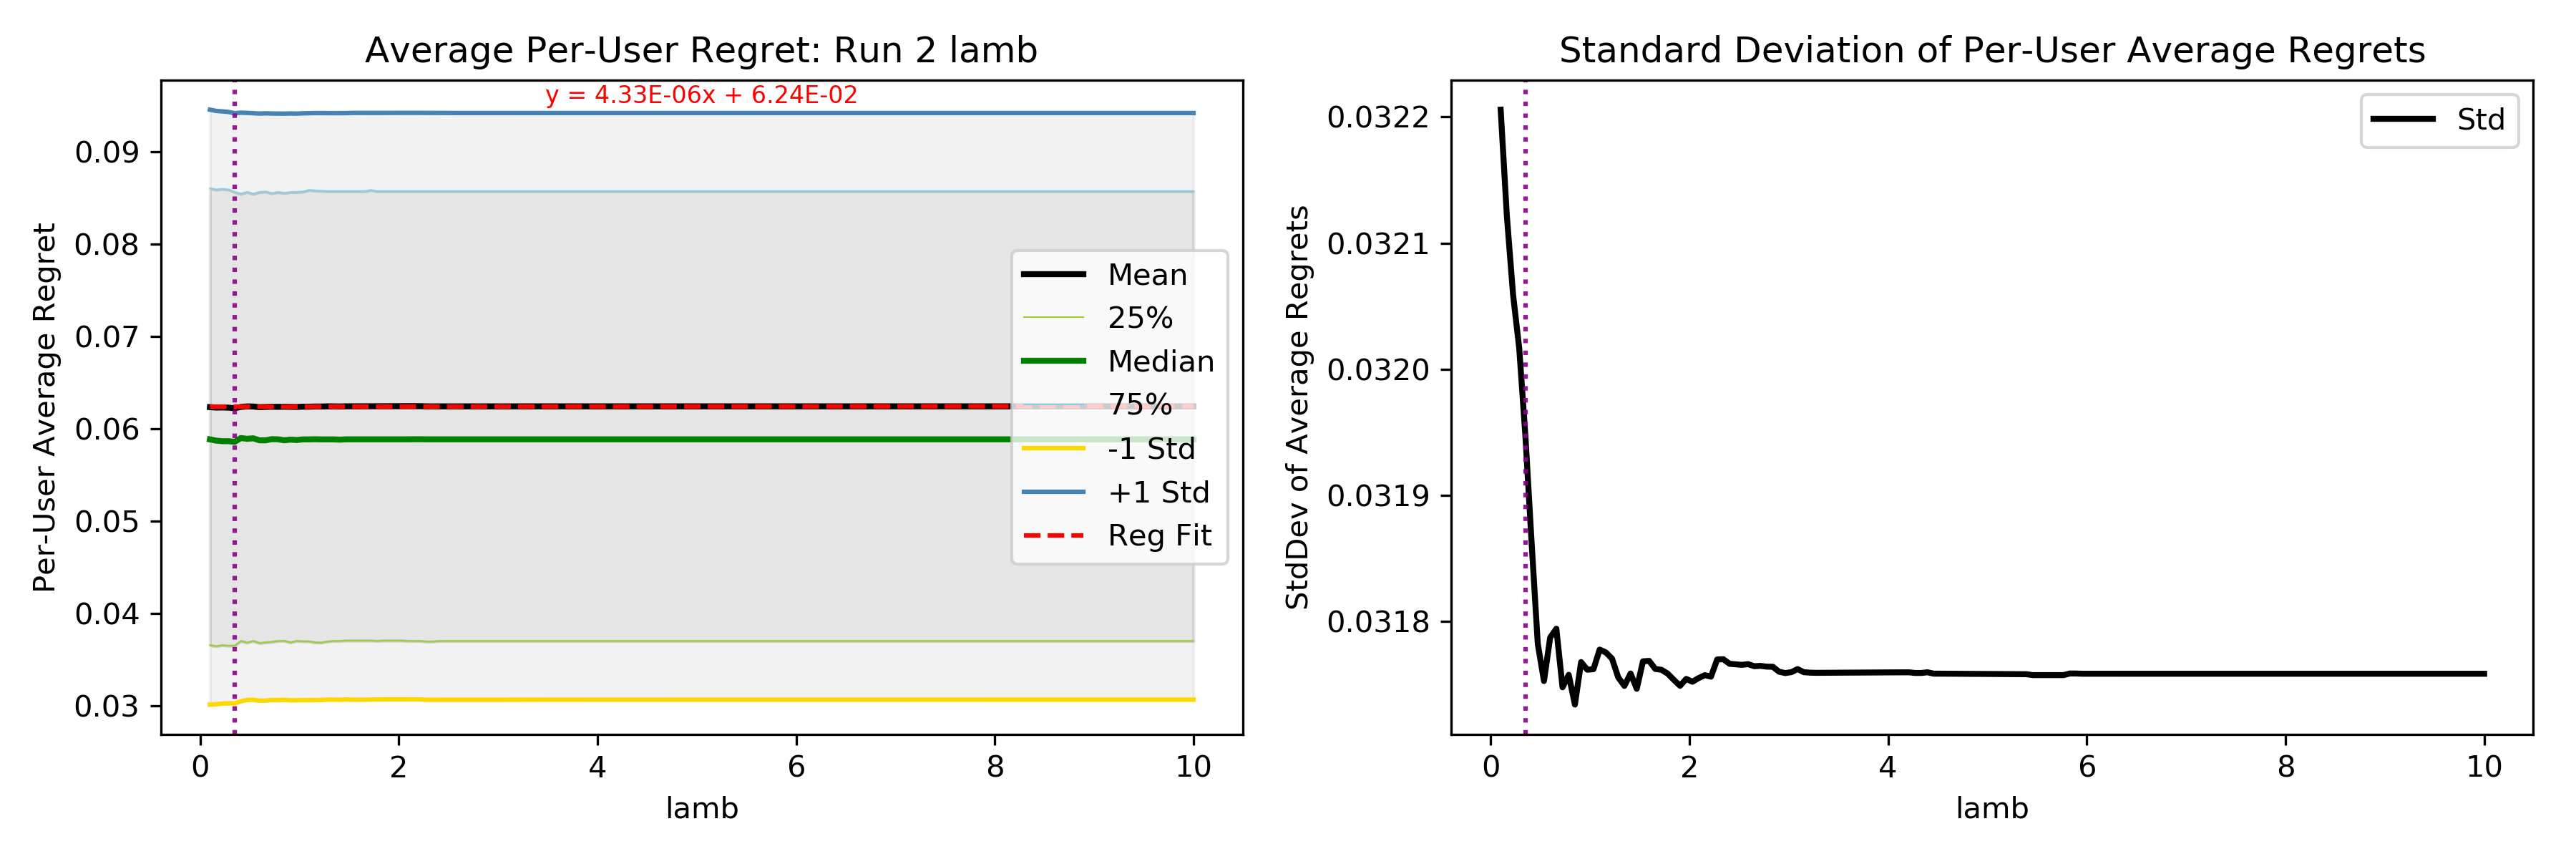
\includegraphics[width=1.1\textwidth,center]{figures/opt_param/opt_param_11100_lamb2.png}%
	\newline
	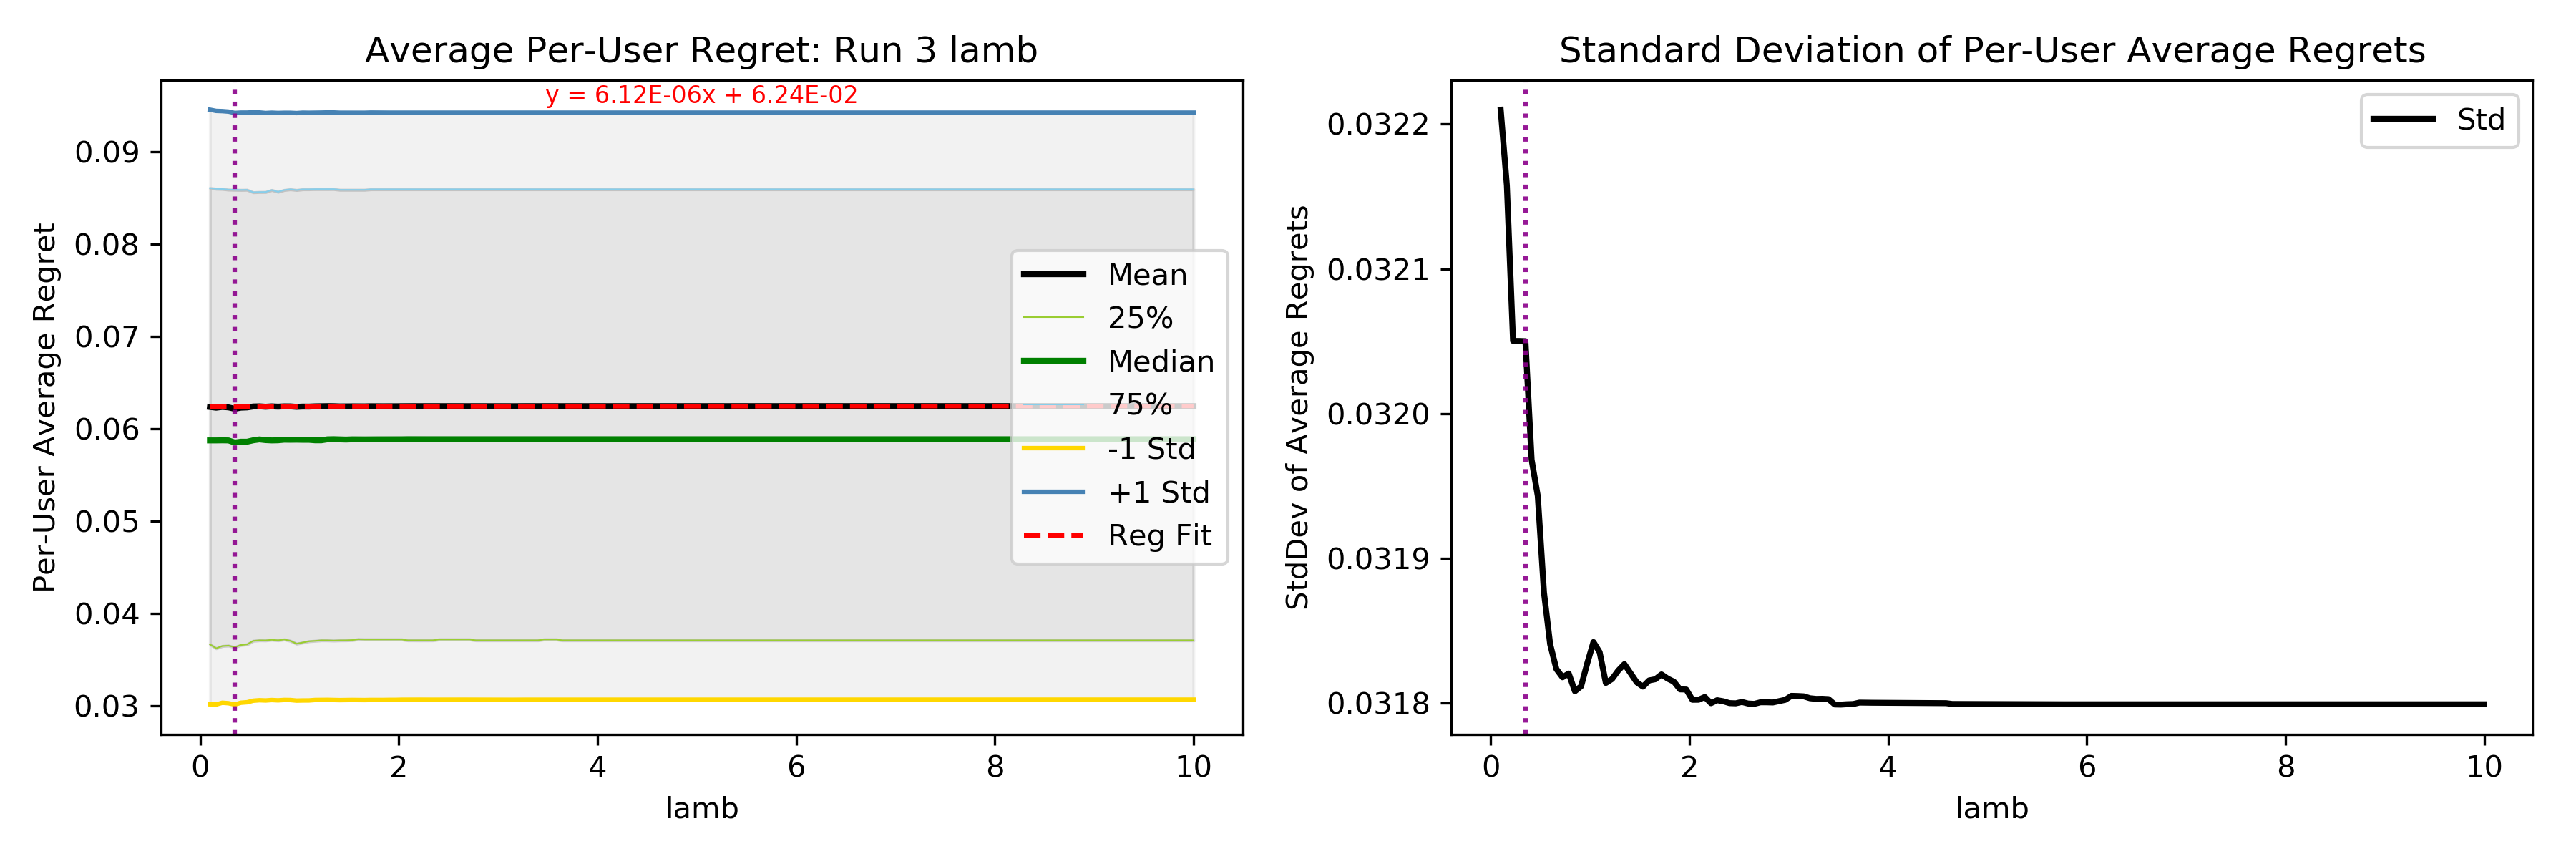
\includegraphics[width=1.1\textwidth,center]{figures/opt_param/opt_param_11100_lamb3.png}%
	\newline
	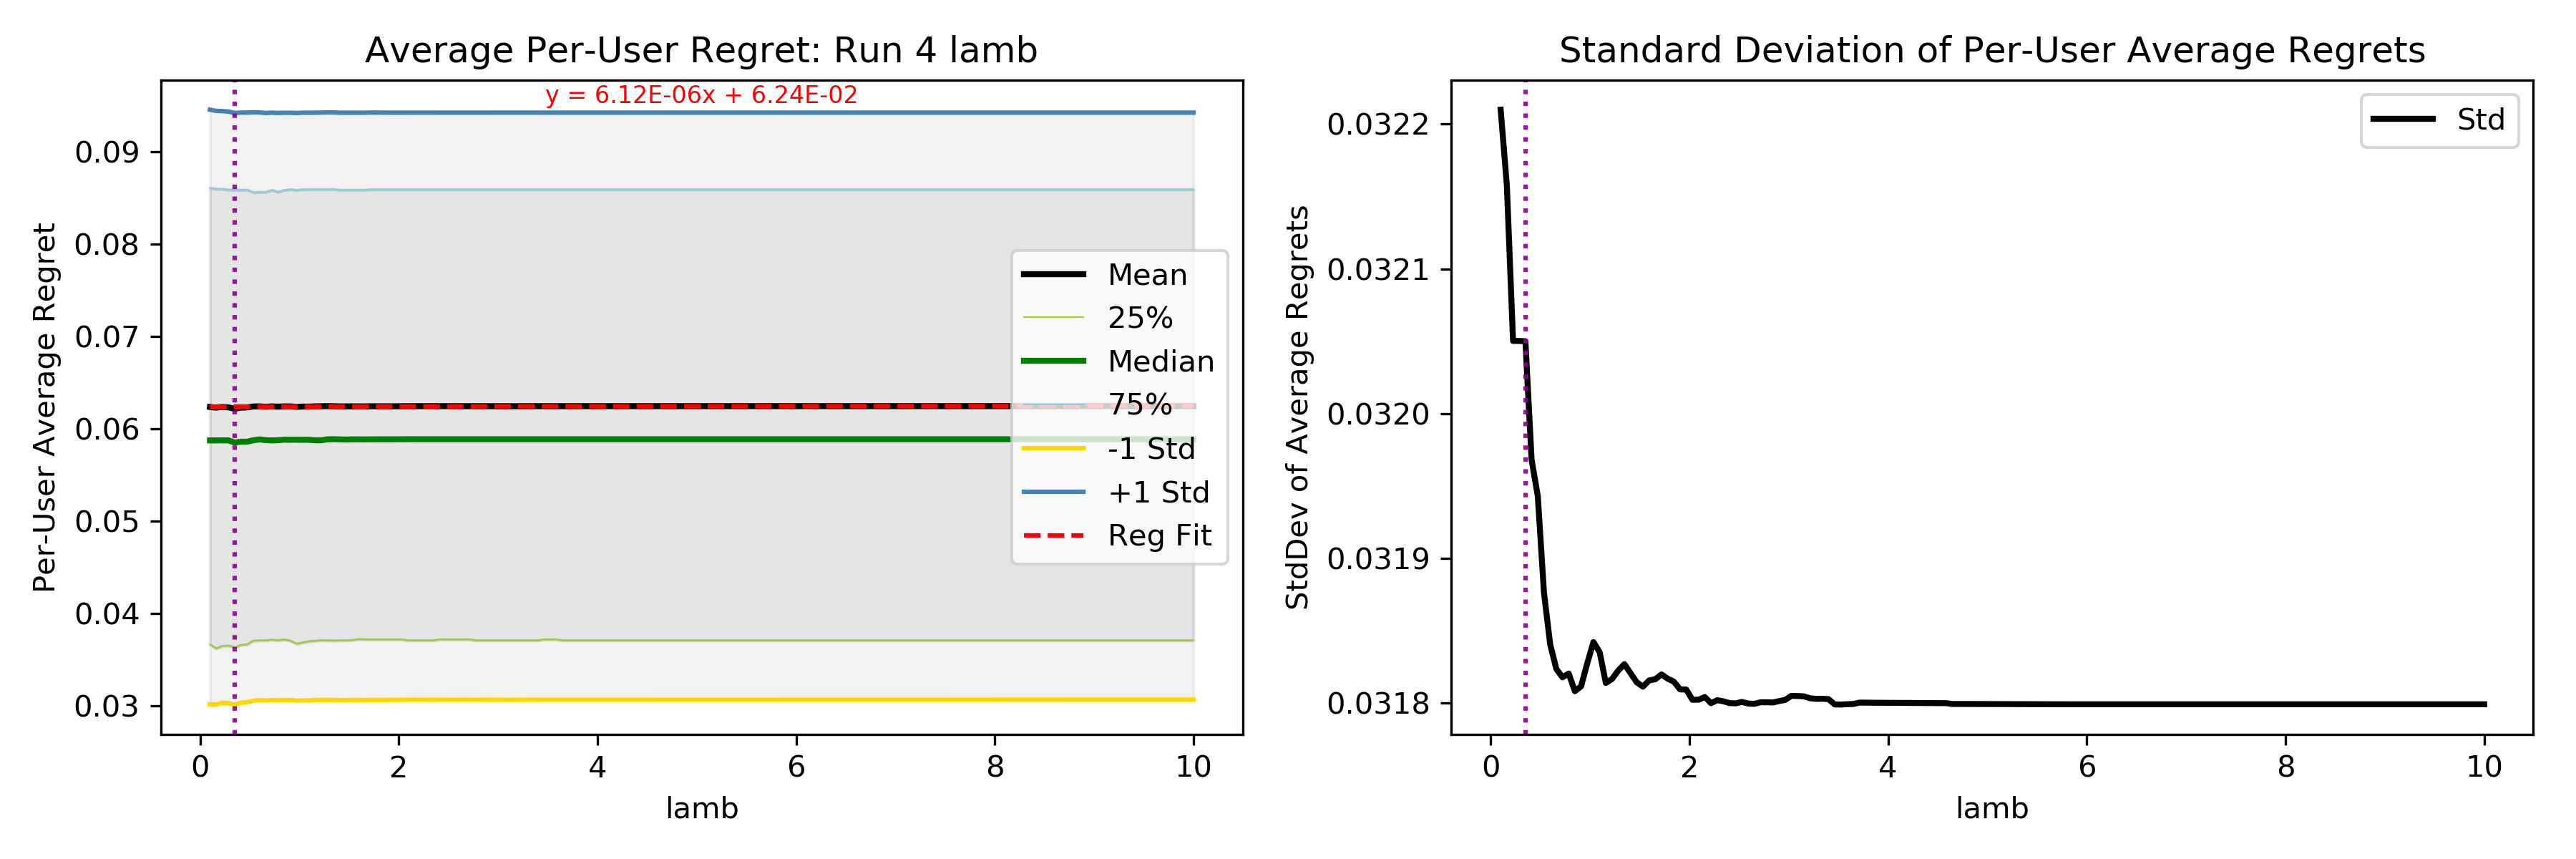
\includegraphics[width=1.1\textwidth,center]{figures/opt_param/opt_param_11100_lamb4.png}%
	\caption{$MUER$ for Varying $\mathtt{lamb}$, $MUER$ Minimization Optimization}
	\end{figure}

	\begin{figure}[H]
	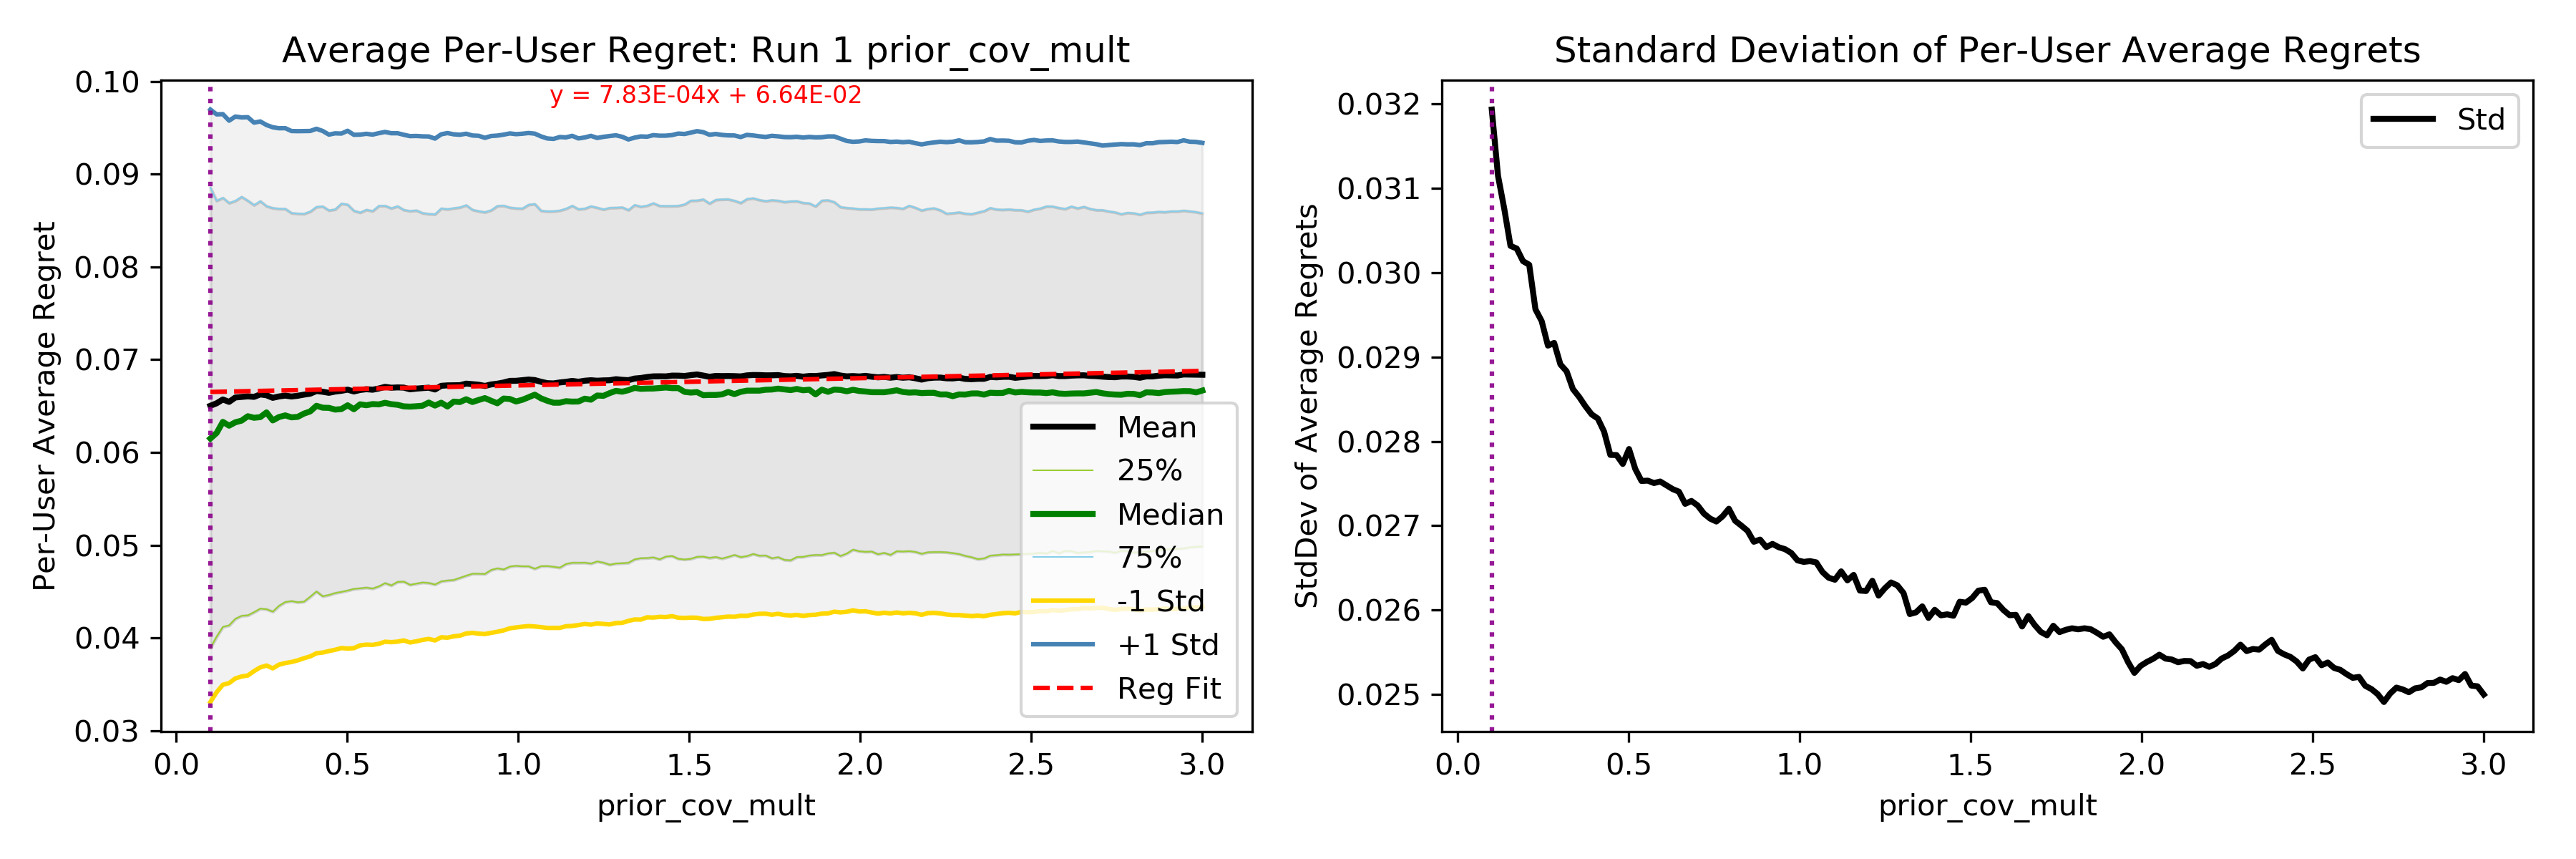
\includegraphics[width=1.1\textwidth,center]{figures/opt_param/opt_param_11100_prior_cov_mult1.png}%
	\newline
	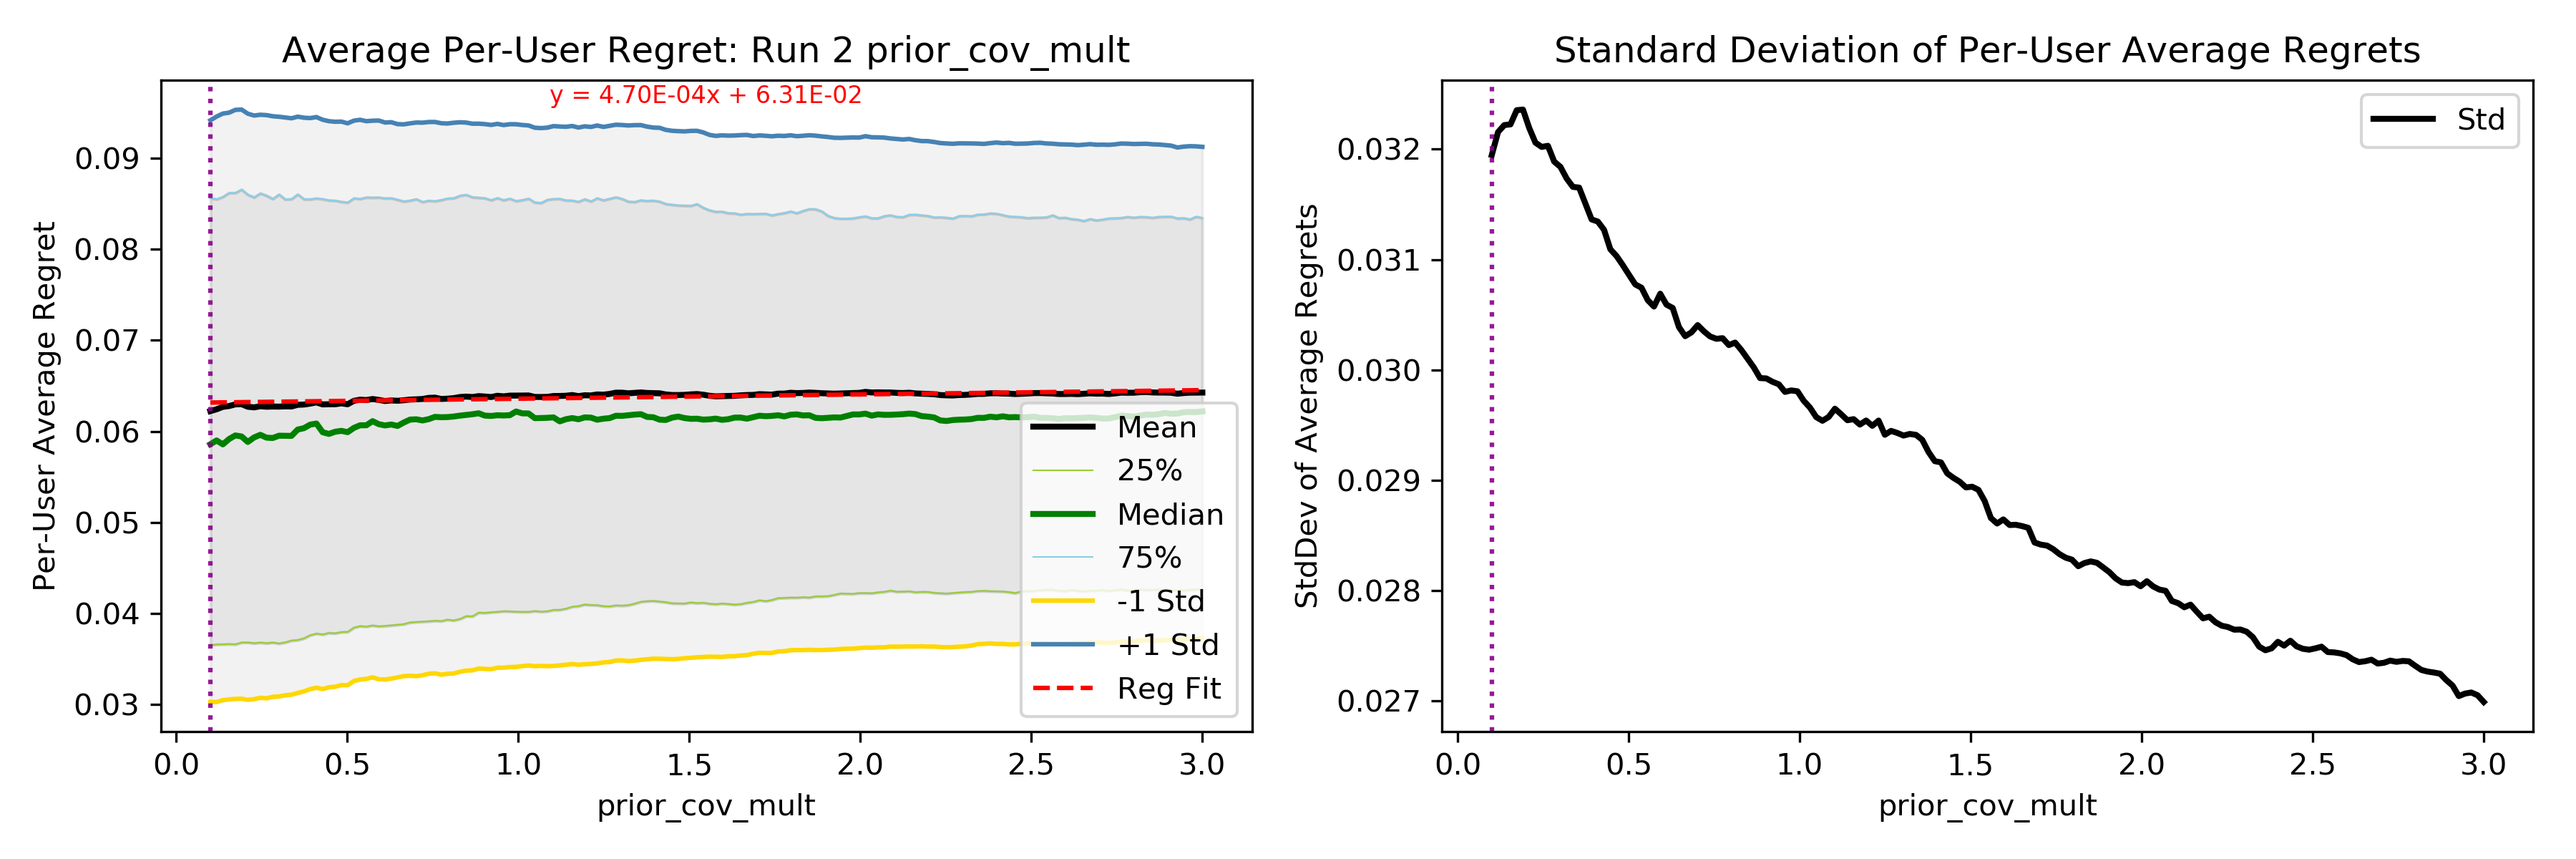
\includegraphics[width=1.1\textwidth,center]{figures/opt_param/opt_param_11100_prior_cov_mult2.png}%
	\newline
	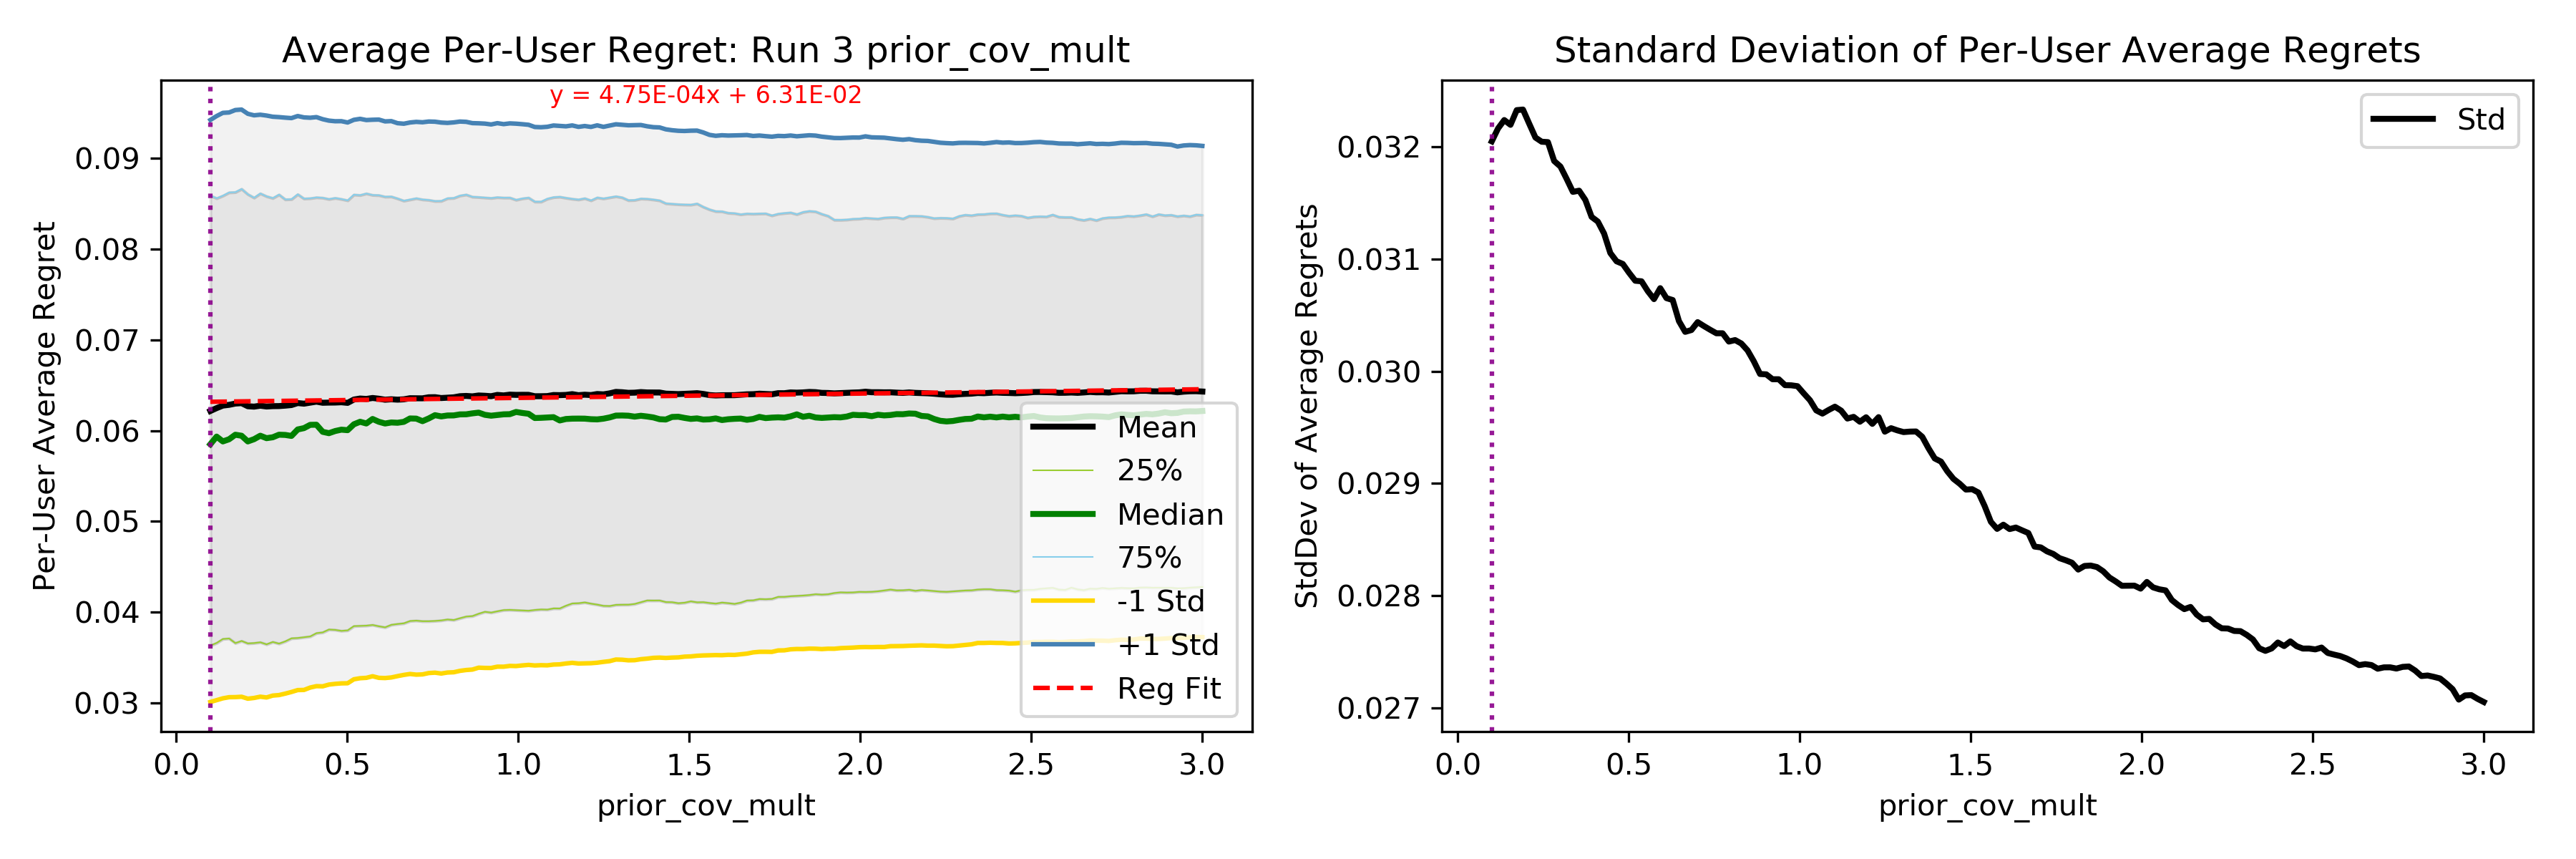
\includegraphics[width=1.1\textwidth,center]{figures/opt_param/opt_param_11100_prior_cov_mult3.png}%
	\newline
	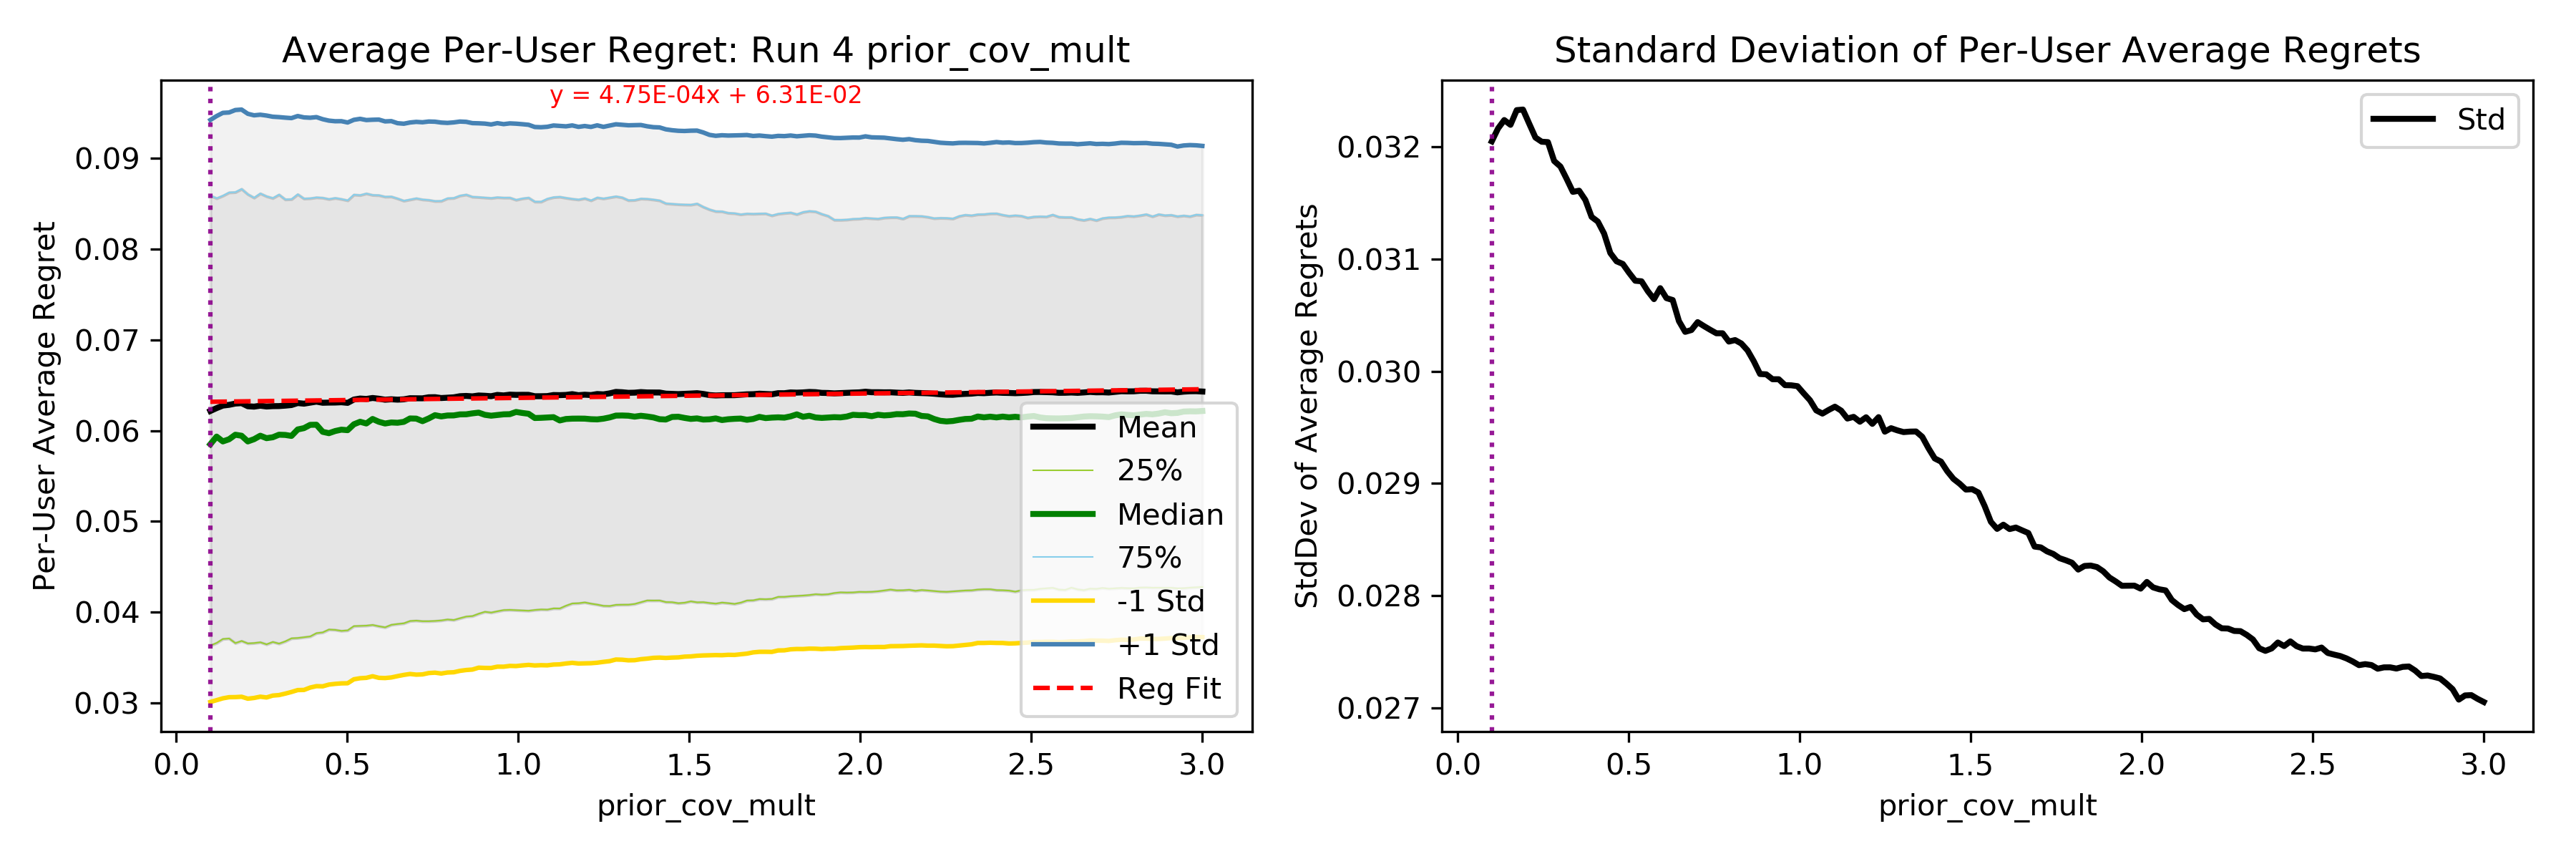
\includegraphics[width=1.1\textwidth,center]{figures/opt_param/opt_param_11100_prior_cov_mult4.png}%
	\caption{$MUER$ for Varying $\mathtt{prior\_cov\_mult}$, $MUER$ Minimization Optimization}
	\end{figure}

	\fi
	%%%%%%%%%%%%%%%%%%%%%%%%%%%%%%%%%%%%%%%%%%%%%%%%%%%%%%%%%%%%%%%




\subsection{Standard Deviation Cutoff Parameter Optimization}
	\label{Standard Deviation Cutoff Parameter Optimization}

	\ifdraft
	Turn off Draft mode to display figures!
	\else
	%%%%%%%%%%%%%%%%%%%%%%%%%%%%%%%%%%%%%%%%%%%%%%%%%%%%%%%%%%%%%%%%

	\begin{figure}[H]
	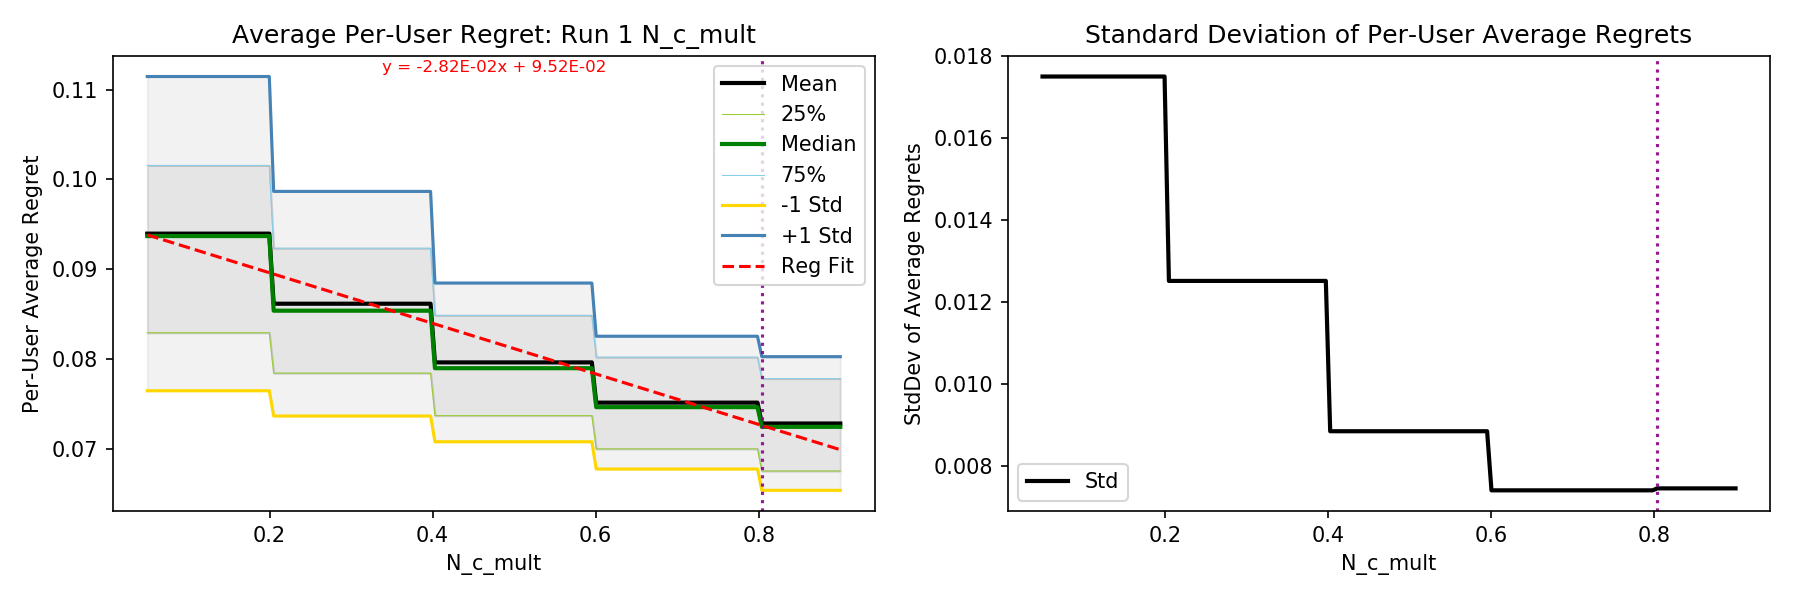
\includegraphics[width=1.1\textwidth,center]{figures/opt_param/opt_param_std_11100_N_c_mult1.png}%
	\newline
	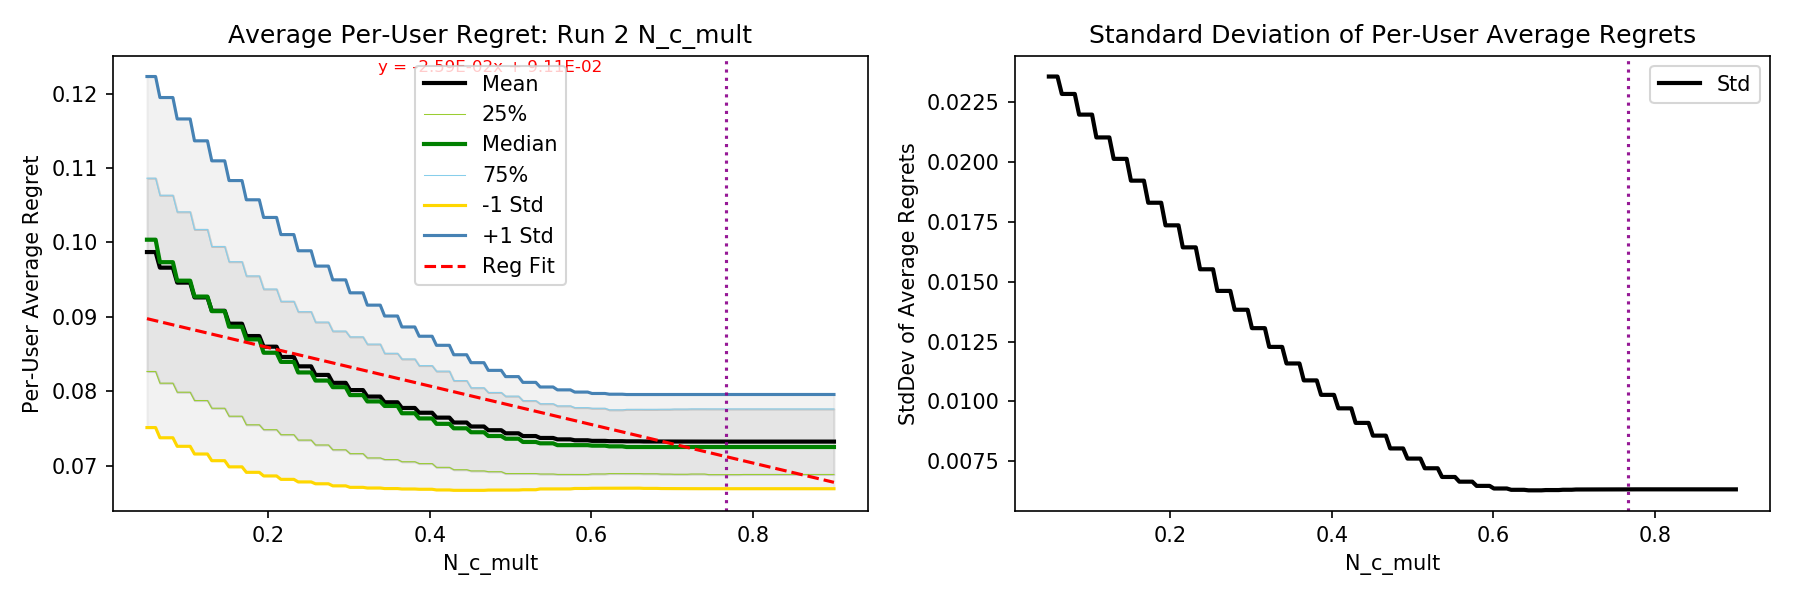
\includegraphics[width=1.1\textwidth,center]{figures/opt_param/opt_param_std_11100_N_c_mult2.png}%
	\newline
	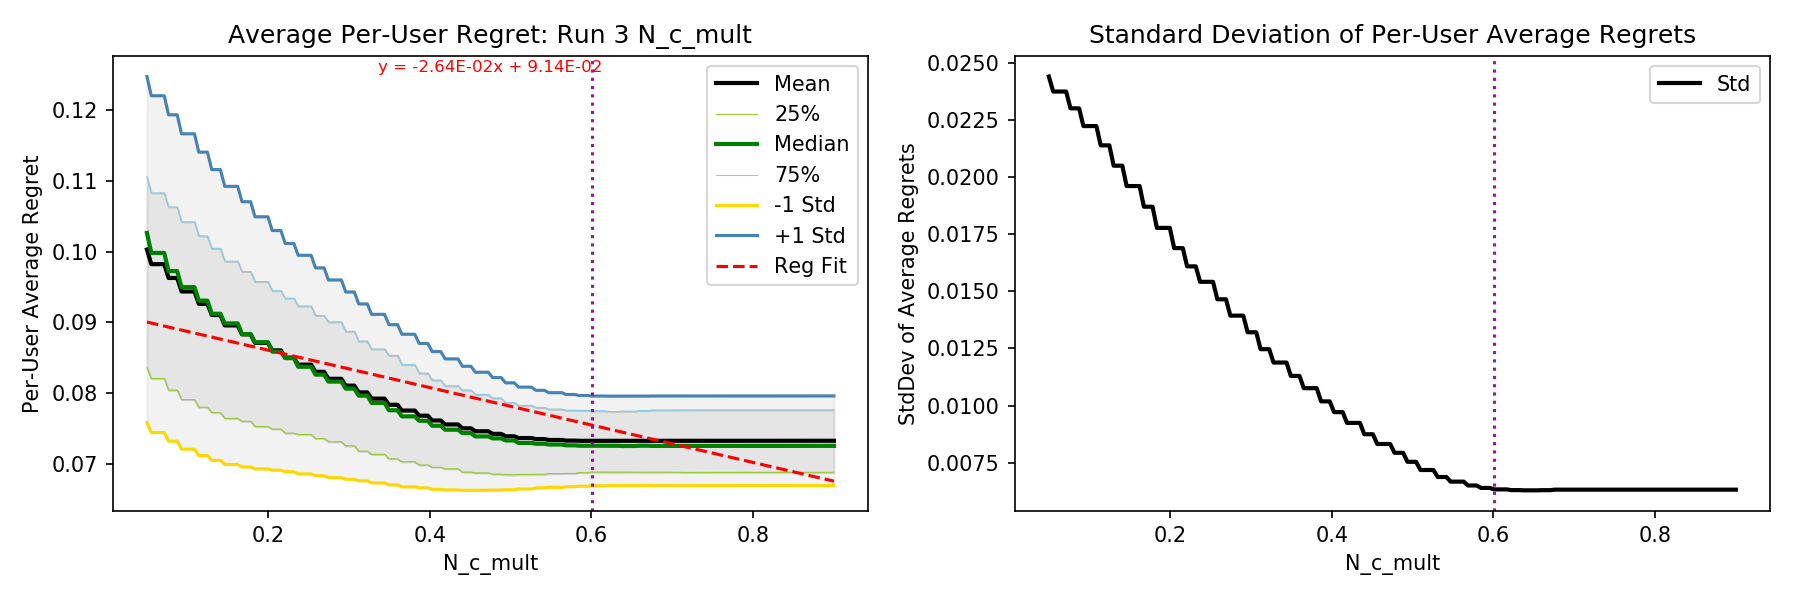
\includegraphics[width=1.1\textwidth,center]{figures/opt_param/opt_param_std_11100_N_c_mult3.png}%
	\newline
	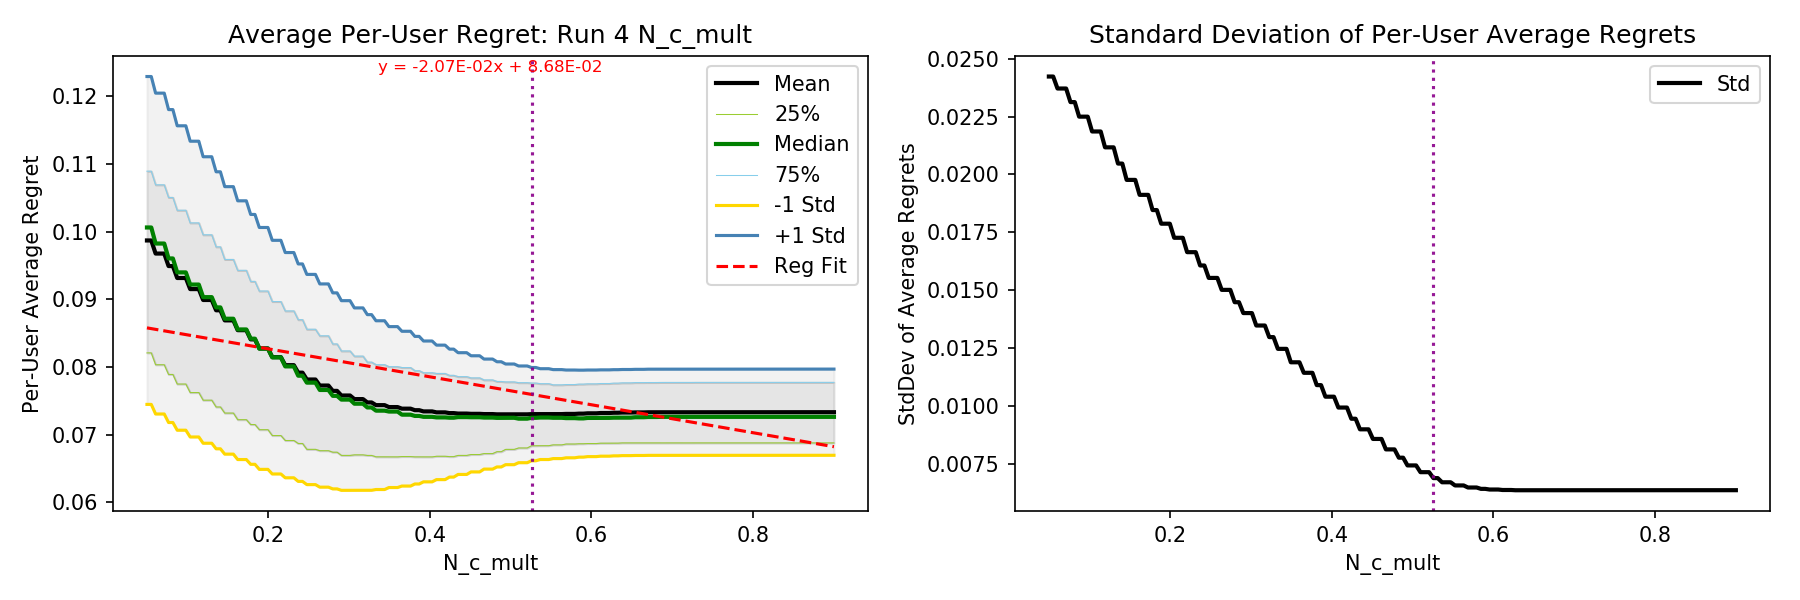
\includegraphics[width=1.1\textwidth,center]{figures/opt_param/opt_param_std_11100_N_c_mult4.png}%
	\caption{$MUER$ for Varying $\mathtt{N\_c\_mult}$, StdDev Cutoff Optimization}
	\end{figure}

	\begin{figure}[H]
	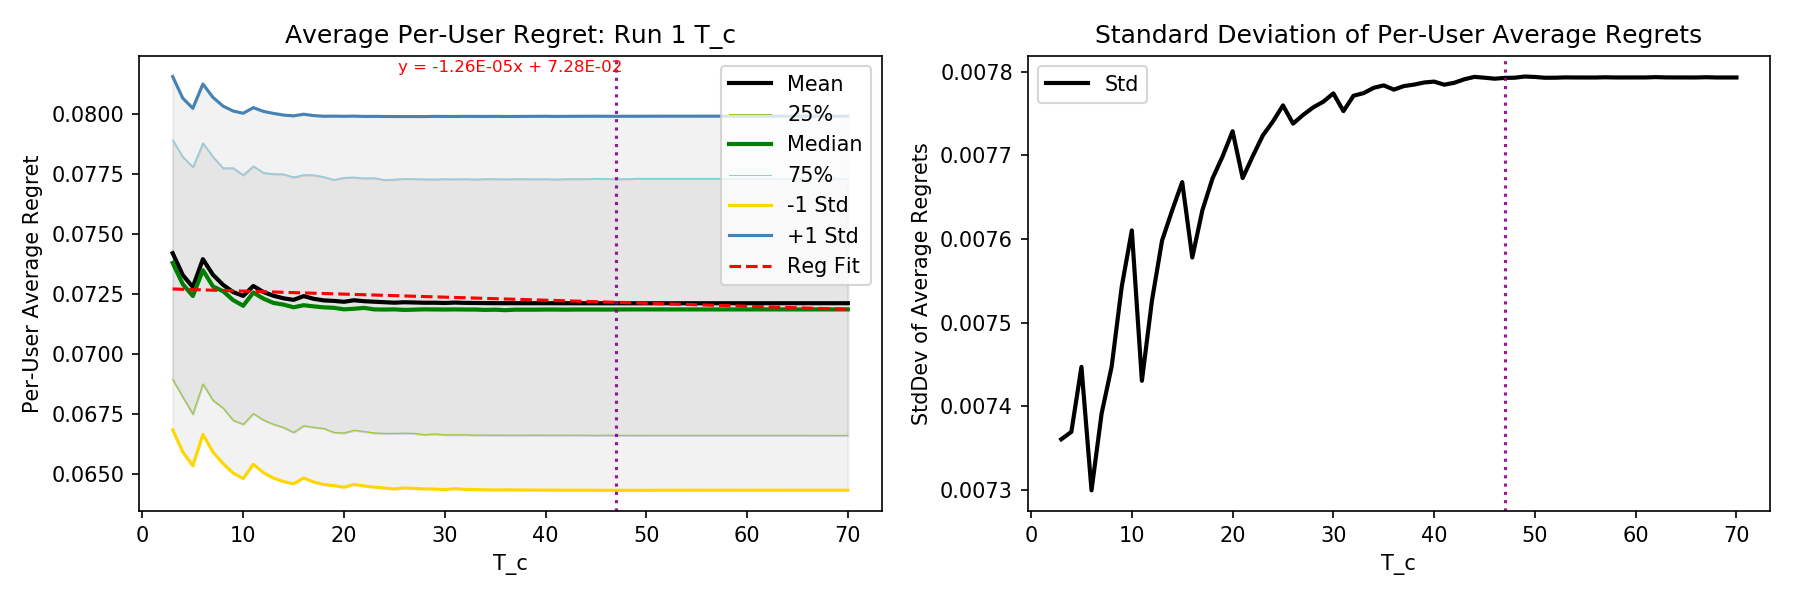
\includegraphics[width=1.1\textwidth,center]{figures/opt_param/opt_param_std_11100_T_c1.png}%
	\newline
	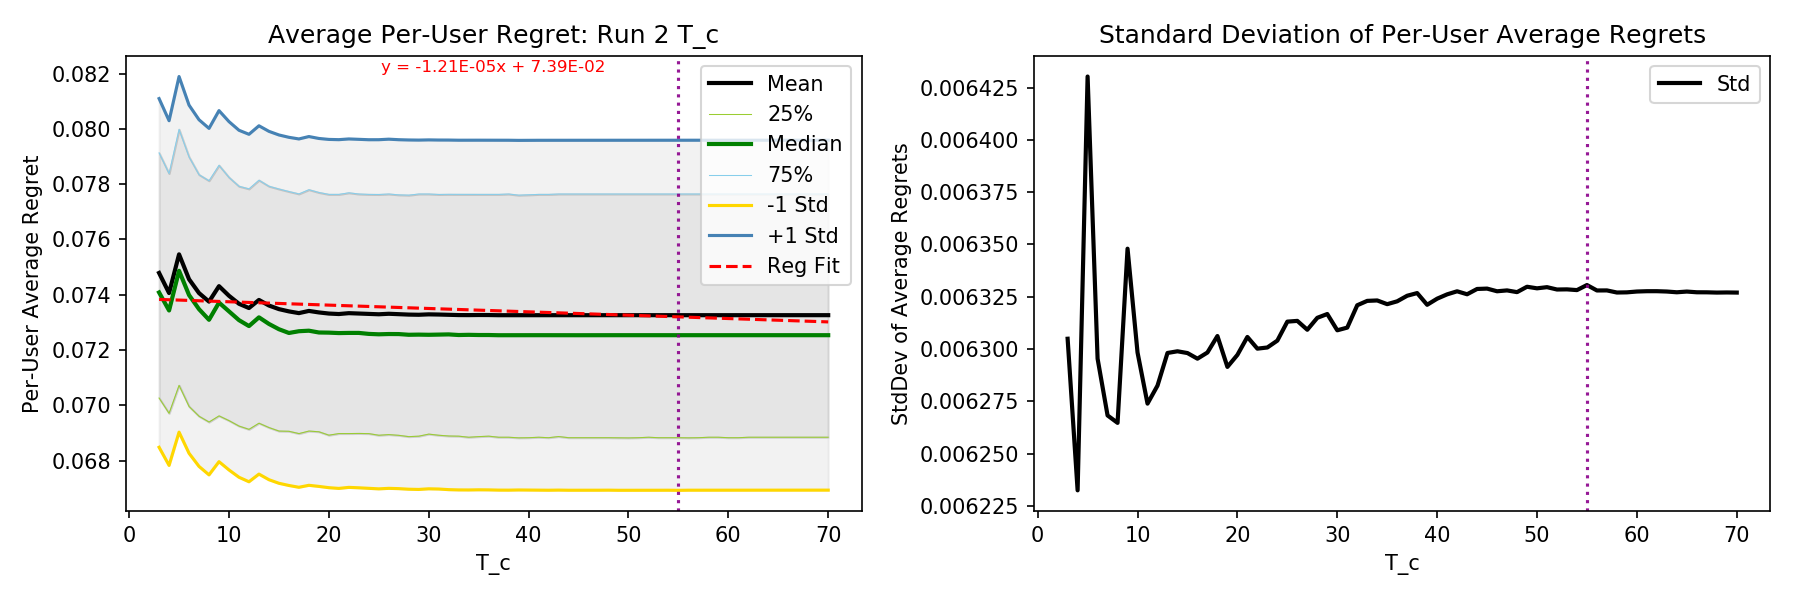
\includegraphics[width=1.1\textwidth,center]{figures/opt_param/opt_param_std_11100_T_c2.png}%
	\newline
	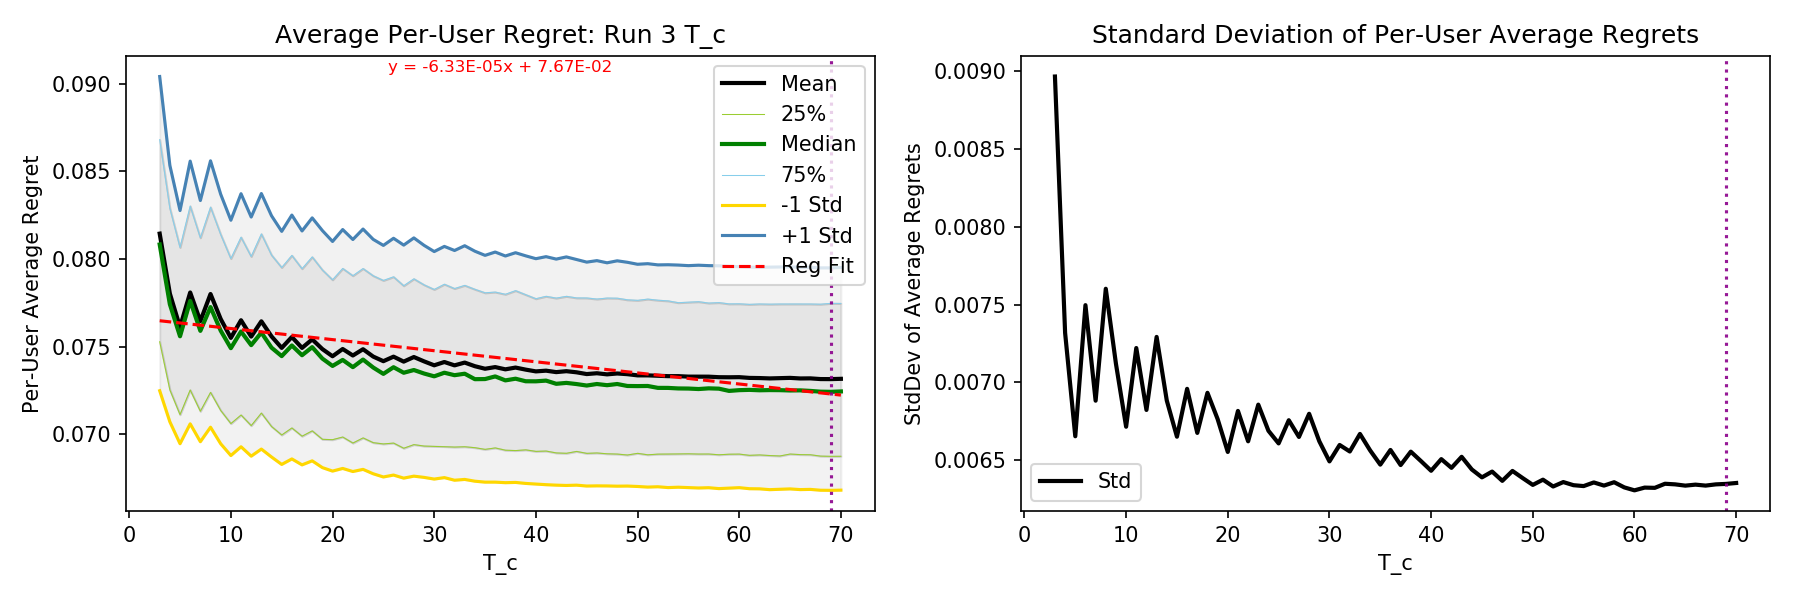
\includegraphics[width=1.1\textwidth,center]{figures/opt_param/opt_param_std_11100_T_c3.png}%
	\newline
	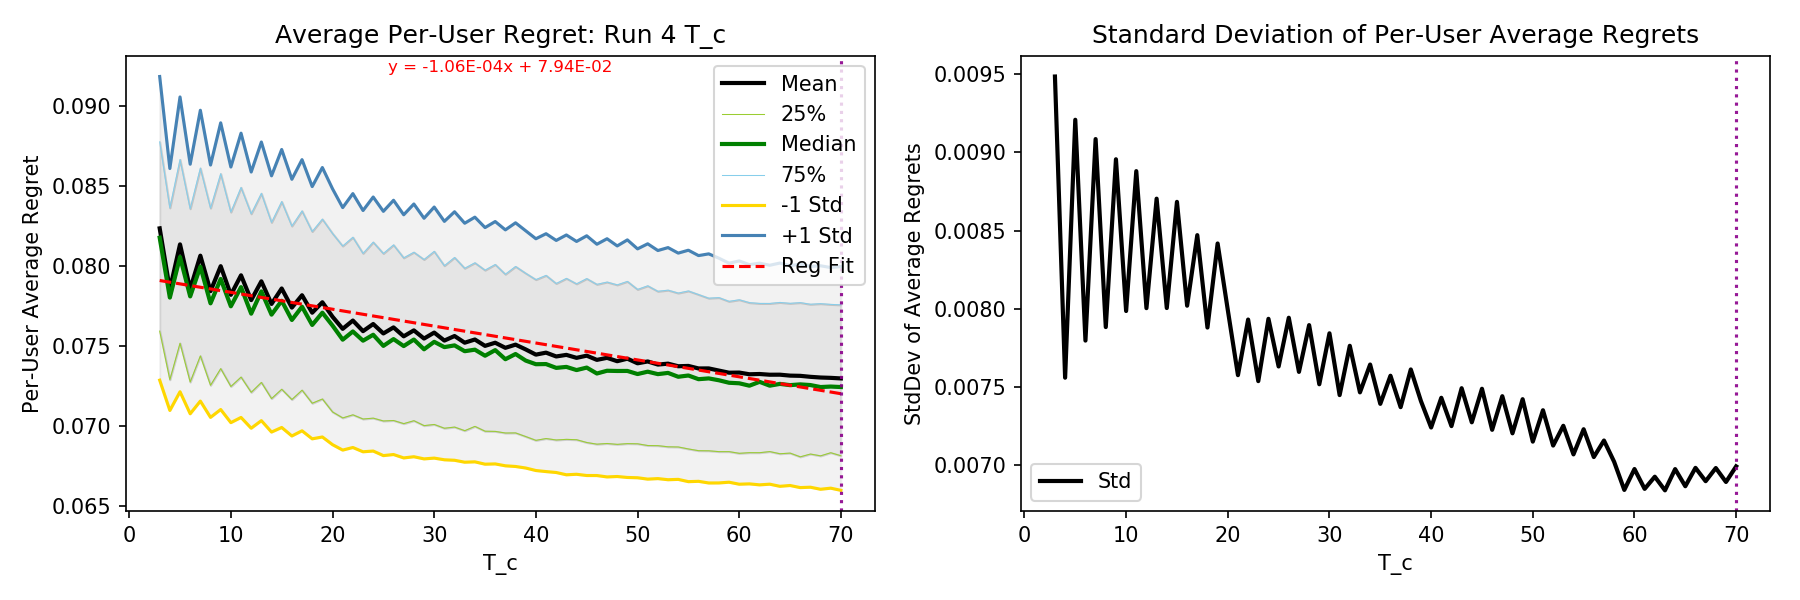
\includegraphics[width=1.1\textwidth,center]{figures/opt_param/opt_param_std_11100_T_c4.png}%
	\caption{$MUER$ for Varying $\mathtt{T\_c}$, StdDev Cutoff Optimization}
	\end{figure}

	\begin{figure}[H]
	\includegraphics[width=1.1\textwidth,center]{figures/opt_param/opt_param_std_11100_sig2_mult1.png}%
	\newline
	\includegraphics[width=1.1\textwidth,center]{figures/opt_param/opt_param_std_11100_sig2_mult2.png}%
	\newline
	\includegraphics[width=1.1\textwidth,center]{figures/opt_param/opt_param_std_11100_sig2_mult3.png}%
	\newline
	\includegraphics[width=1.1\textwidth,center]{figures/opt_param/opt_param_std_11100_sig2_mult4.png}%
	\caption{$MUER$ for Varying $\mathtt{sig2\_mult}$, StdDev Cutoff Optimization}
	\end{figure}

	\begin{figure}[H]
	\includegraphics[width=1.1\textwidth,center]{figures/opt_param/opt_param_std_11100_gamma1.png}%
	\newline
	\includegraphics[width=1.1\textwidth,center]{figures/opt_param/opt_param_std_11100_gamma2.png}%
	\newline
	\includegraphics[width=1.1\textwidth,center]{figures/opt_param/opt_param_std_11100_gamma3.png}%
	\newline
	\includegraphics[width=1.1\textwidth,center]{figures/opt_param/opt_param_std_11100_gamma4.png}%
	\caption{$MUER$ for Varying $\mathtt{gamma}$, StdDev Cutoff Optimization}
	\end{figure}

	\begin{figure}[H]
	\includegraphics[width=1.1\textwidth,center]{figures/opt_param/opt_param_std_11100_lamb1.png}%
	\newline
	\includegraphics[width=1.1\textwidth,center]{figures/opt_param/opt_param_std_11100_lamb2.png}%
	\newline
	\includegraphics[width=1.1\textwidth,center]{figures/opt_param/opt_param_std_11100_lamb3.png}%
	\newline
	\includegraphics[width=1.1\textwidth,center]{figures/opt_param/opt_param_std_11100_lamb4.png}%
	\caption{$MUER$ for Varying $\mathtt{lamb}$, StdDev Cutoff Optimization}
	\end{figure}

	\begin{figure}[H]
	\includegraphics[width=1.1\textwidth,center]{figures/opt_param/opt_param_std_11100_prior_cov_mult1.png}%
	\newline
	\includegraphics[width=1.1\textwidth,center]{figures/opt_param/opt_param_std_11100_prior_cov_mult2.png}%
	\newline
	\includegraphics[width=1.1\textwidth,center]{figures/opt_param/opt_param_std_11100_prior_cov_mult3.png}%
	\newline
	\includegraphics[width=1.1\textwidth,center]{figures/opt_param/opt_param_std_11100_prior_cov_mult4.png}%
	\caption{$MUER$ for Varying $\mathtt{prior\_cov\_mult}$, StdDev Cutoff Optimization}
	\end{figure}
	\fi


​

%%%%%%%%%%%%%%%%%%%%%%%%%%%%%%%%%%%%%%%%%%%%%%%%%%%%%%%%%%%%%%%%